% Options for packages loaded elsewhere
\PassOptionsToPackage{unicode}{hyperref}
\PassOptionsToPackage{hyphens}{url}
%
\documentclass[
]{book}
\usepackage{lmodern}
\usepackage{amssymb,amsmath}
\usepackage{ifxetex,ifluatex}
\ifnum 0\ifxetex 1\fi\ifluatex 1\fi=0 % if pdftex
  \usepackage[T1]{fontenc}
  \usepackage[utf8]{inputenc}
  \usepackage{textcomp} % provide euro and other symbols
\else % if luatex or xetex
  \usepackage{unicode-math}
  \defaultfontfeatures{Scale=MatchLowercase}
  \defaultfontfeatures[\rmfamily]{Ligatures=TeX,Scale=1}
\fi
% Use upquote if available, for straight quotes in verbatim environments
\IfFileExists{upquote.sty}{\usepackage{upquote}}{}
\IfFileExists{microtype.sty}{% use microtype if available
  \usepackage[]{microtype}
  \UseMicrotypeSet[protrusion]{basicmath} % disable protrusion for tt fonts
}{}
\makeatletter
\@ifundefined{KOMAClassName}{% if non-KOMA class
  \IfFileExists{parskip.sty}{%
    \usepackage{parskip}
  }{% else
    \setlength{\parindent}{0pt}
    \setlength{\parskip}{6pt plus 2pt minus 1pt}}
}{% if KOMA class
  \KOMAoptions{parskip=half}}
\makeatother
\usepackage{xcolor}
\IfFileExists{xurl.sty}{\usepackage{xurl}}{} % add URL line breaks if available
\IfFileExists{bookmark.sty}{\usepackage{bookmark}}{\usepackage{hyperref}}
\hypersetup{
  pdftitle={Notas de aulas de Estatística Econômica},
  pdfauthor={Marcos Minoru Hasegawa},
  hidelinks,
  pdfcreator={LaTeX via pandoc}}
\urlstyle{same} % disable monospaced font for URLs
\usepackage{color}
\usepackage{fancyvrb}
\newcommand{\VerbBar}{|}
\newcommand{\VERB}{\Verb[commandchars=\\\{\}]}
\DefineVerbatimEnvironment{Highlighting}{Verbatim}{commandchars=\\\{\}}
% Add ',fontsize=\small' for more characters per line
\usepackage{framed}
\definecolor{shadecolor}{RGB}{248,248,248}
\newenvironment{Shaded}{\begin{snugshade}}{\end{snugshade}}
\newcommand{\AlertTok}[1]{\textcolor[rgb]{0.94,0.16,0.16}{#1}}
\newcommand{\AnnotationTok}[1]{\textcolor[rgb]{0.56,0.35,0.01}{\textbf{\textit{#1}}}}
\newcommand{\AttributeTok}[1]{\textcolor[rgb]{0.77,0.63,0.00}{#1}}
\newcommand{\BaseNTok}[1]{\textcolor[rgb]{0.00,0.00,0.81}{#1}}
\newcommand{\BuiltInTok}[1]{#1}
\newcommand{\CharTok}[1]{\textcolor[rgb]{0.31,0.60,0.02}{#1}}
\newcommand{\CommentTok}[1]{\textcolor[rgb]{0.56,0.35,0.01}{\textit{#1}}}
\newcommand{\CommentVarTok}[1]{\textcolor[rgb]{0.56,0.35,0.01}{\textbf{\textit{#1}}}}
\newcommand{\ConstantTok}[1]{\textcolor[rgb]{0.00,0.00,0.00}{#1}}
\newcommand{\ControlFlowTok}[1]{\textcolor[rgb]{0.13,0.29,0.53}{\textbf{#1}}}
\newcommand{\DataTypeTok}[1]{\textcolor[rgb]{0.13,0.29,0.53}{#1}}
\newcommand{\DecValTok}[1]{\textcolor[rgb]{0.00,0.00,0.81}{#1}}
\newcommand{\DocumentationTok}[1]{\textcolor[rgb]{0.56,0.35,0.01}{\textbf{\textit{#1}}}}
\newcommand{\ErrorTok}[1]{\textcolor[rgb]{0.64,0.00,0.00}{\textbf{#1}}}
\newcommand{\ExtensionTok}[1]{#1}
\newcommand{\FloatTok}[1]{\textcolor[rgb]{0.00,0.00,0.81}{#1}}
\newcommand{\FunctionTok}[1]{\textcolor[rgb]{0.00,0.00,0.00}{#1}}
\newcommand{\ImportTok}[1]{#1}
\newcommand{\InformationTok}[1]{\textcolor[rgb]{0.56,0.35,0.01}{\textbf{\textit{#1}}}}
\newcommand{\KeywordTok}[1]{\textcolor[rgb]{0.13,0.29,0.53}{\textbf{#1}}}
\newcommand{\NormalTok}[1]{#1}
\newcommand{\OperatorTok}[1]{\textcolor[rgb]{0.81,0.36,0.00}{\textbf{#1}}}
\newcommand{\OtherTok}[1]{\textcolor[rgb]{0.56,0.35,0.01}{#1}}
\newcommand{\PreprocessorTok}[1]{\textcolor[rgb]{0.56,0.35,0.01}{\textit{#1}}}
\newcommand{\RegionMarkerTok}[1]{#1}
\newcommand{\SpecialCharTok}[1]{\textcolor[rgb]{0.00,0.00,0.00}{#1}}
\newcommand{\SpecialStringTok}[1]{\textcolor[rgb]{0.31,0.60,0.02}{#1}}
\newcommand{\StringTok}[1]{\textcolor[rgb]{0.31,0.60,0.02}{#1}}
\newcommand{\VariableTok}[1]{\textcolor[rgb]{0.00,0.00,0.00}{#1}}
\newcommand{\VerbatimStringTok}[1]{\textcolor[rgb]{0.31,0.60,0.02}{#1}}
\newcommand{\WarningTok}[1]{\textcolor[rgb]{0.56,0.35,0.01}{\textbf{\textit{#1}}}}
\usepackage{longtable,booktabs}
% Correct order of tables after \paragraph or \subparagraph
\usepackage{etoolbox}
\makeatletter
\patchcmd\longtable{\par}{\if@noskipsec\mbox{}\fi\par}{}{}
\makeatother
% Allow footnotes in longtable head/foot
\IfFileExists{footnotehyper.sty}{\usepackage{footnotehyper}}{\usepackage{footnote}}
\makesavenoteenv{longtable}
\usepackage{graphicx,grffile}
\makeatletter
\def\maxwidth{\ifdim\Gin@nat@width>\linewidth\linewidth\else\Gin@nat@width\fi}
\def\maxheight{\ifdim\Gin@nat@height>\textheight\textheight\else\Gin@nat@height\fi}
\makeatother
% Scale images if necessary, so that they will not overflow the page
% margins by default, and it is still possible to overwrite the defaults
% using explicit options in \includegraphics[width, height, ...]{}
\setkeys{Gin}{width=\maxwidth,height=\maxheight,keepaspectratio}
% Set default figure placement to htbp
\makeatletter
\def\fps@figure{htbp}
\makeatother
\setlength{\emergencystretch}{3em} % prevent overfull lines
\providecommand{\tightlist}{%
  \setlength{\itemsep}{0pt}\setlength{\parskip}{0pt}}
\setcounter{secnumdepth}{5}
\usepackage[brazil]{babel}
\usepackage[utf8]{inputenc}
\usepackage[T1]{fontenc}
\usepackage{lmodern}
\usepackage{amsmath,amssymb,amsthm,adjustbox,mathtools,bm,cool}
\usepackage{natbib}
\usepackage{graphics,graphicx,import,color,float}
\usepackage{url,booktabs,siunitx}
\usepackage{xcolor}
\usepackage[]{natbib}
\bibliographystyle{apalike}

\title{Notas de aulas de Estatística Econômica}
\author{Marcos Minoru Hasegawa}
\date{2020-11-16}

\begin{document}
\maketitle

{
\setcounter{tocdepth}{1}
\tableofcontents
}
\hypertarget{licenuxe7a}{%
\chapter*{Licença}\label{licenuxe7a}}
\addcontentsline{toc}{chapter}{Licença}

Como está descrito no repositório, os poucos códigos originais desenvolvidos ao longo do texto estão sob a licença \textbf{GNU GPLv3} .

O texto e as artes gráficas elaboradas de forma original estão sob licença \textbf{Creative Commons BY-NC-SA 4.0}.

\hypertarget{sobre-o-material}{%
\chapter*{Sobre o material}\label{sobre-o-material}}
\addcontentsline{toc}{chapter}{Sobre o material}

A situação especial causada pela pandemia da COVID-19 forçou a muitos professores criarem materiais para facilitar aulas remotas das suas disciplinas. A disciplina SE305 Estatística Econômica e Introdução à Econometria da UFPR não poderia ser diferente. Então, o objetivo deste material é de suprir a falta das bibliografias básicas na sua versão digital com a disponibilização de forma digital e gratuita o que seria o material das notas das aulas da disciplina de Estatística Econômica. Não é o ideal, mas a ideia é melhorar o material com tempo.

\hypertarget{sobre-o-autor}{%
\chapter*{Sobre o Autor}\label{sobre-o-autor}}
\addcontentsline{toc}{chapter}{Sobre o Autor}

Professor do Departamento de Economia da Universidade Federal do Paraná. Engenheiro Agrônomo pela UNESP/Jaboticabal, Mestrado em Economia Agrária pela ESALQ/USP e Doutorado em Economia Aplicada pela ESALQ/USP, é um dos professores responsáveis pelas disciplinas de SE305 Estatística Econômica e Introdução à Econometria e SE308 Econometria ambas do curso de Economia da Universidade Federal do Paraná (UFPR).

\hypertarget{estatuxedstica-descritiva}{%
\chapter{Estatística Descritiva}\label{estatuxedstica-descritiva}}

O conteúdo deste tópico foi elaborado com base no capitulo 2 de \citet{Sartoris2013} e nos capítulos 4 e 5 de \citet{Hoffmann2006}.

\hypertarget{medidas-de-posiuxe7uxe3o}{%
\section{Medidas de posição}\label{medidas-de-posiuxe7uxe3o}}

Trata-se de medidas de tendência central ou resumo. Como os nomes dizem, tratam-se de medidas que tratam de resumir a massa de valores e um único número.

\hypertarget{variuxe1vel-aleatuxf3ria}{%
\subsection{Variável Aleatória}\label{variuxe1vel-aleatuxf3ria}}

\begin{itemize}
\tightlist
\item
  variável aleatória (v.a.) é uma variável que está associada a uma \emph{distribuição de probabilidade}.
\item
  Ou seja, cada valor da v.a. está associada a uma probabilidade.
\item
  O resultado do lançamento de uma dado, que poder ser qualquer número de 1 a 6, está associada a uma probabilidade de \(1/6\).
\end{itemize}

\hypertarget{muxe9dia-aritmuxe9tica-simples}{%
\subsection{Média Aritmética Simples}\label{muxe9dia-aritmuxe9tica-simples}}

\begin{equation}
    \overline{X} = \frac{1}{n} \sum_{i=1}^{n} X_i
    \label{eq:mediaaritmeticasimples}
\end{equation}
onde \(i =1, ...,n\)

\textbf{Exemplo 1}

Qual é a média aritmética de um grupo de cinco pessoas cujas idades são em ordem crescente, 21,23,25,28 e 31. Para responder, basta aplicar \eqref{eq:mediaaritmeticasimples}.

\begin{equation*}
  \overline{X} = \frac{21+23+25+28+31}{5} = 25,6
\end{equation*}

\textbf{Exemplo 1 no R}

\begin{Shaded}
\begin{Highlighting}[]
\NormalTok{X <-}\StringTok{ }\KeywordTok{c}\NormalTok{(}\DecValTok{21}\NormalTok{, }\DecValTok{23}\NormalTok{, }\DecValTok{25}\NormalTok{, }\DecValTok{28}\NormalTok{, }\DecValTok{31}\NormalTok{)}
\NormalTok{X}
\end{Highlighting}
\end{Shaded}

\begin{verbatim}
## [1] 21 23 25 28 31
\end{verbatim}

\begin{Shaded}
\begin{Highlighting}[]
\NormalTok{mediaX <-}\StringTok{ }\KeywordTok{mean}\NormalTok{(X)}
\NormalTok{mediaX}
\end{Highlighting}
\end{Shaded}

\begin{verbatim}
## [1] 25,6
\end{verbatim}

\textbf{Exemplo 2}

Qual é a média aritmética de três provas realizadas por um aluno, cujas notas
foram 4,6 e 8. Para responder, basta aplicar \eqref{eq:mediaaritmeticasimples}.

\begin{equation*}
  \overline{X} = \frac{4+6+8}{3} = 6
\end{equation*}

\textbf{Exemplo 2 no R}

\begin{Shaded}
\begin{Highlighting}[]
\NormalTok{X2 <-}\StringTok{ }\KeywordTok{c}\NormalTok{(}\DecValTok{4}\NormalTok{, }\DecValTok{6}\NormalTok{, }\DecValTok{8}\NormalTok{)}
\NormalTok{X2}
\end{Highlighting}
\end{Shaded}

\begin{verbatim}
## [1] 4 6 8
\end{verbatim}

\begin{Shaded}
\begin{Highlighting}[]
\NormalTok{mediaX2 <-}\StringTok{ }\KeywordTok{mean}\NormalTok{(X2)}
\NormalTok{mediaX2}
\end{Highlighting}
\end{Shaded}

\begin{verbatim}
## [1] 6
\end{verbatim}

\hypertarget{muxe9dia-aritmuxe9tica-ponderada}{%
\subsection{Média Aritmética Ponderada}\label{muxe9dia-aritmuxe9tica-ponderada}}

Na média aritmética ponderada, cada valor pode ter importância diferentes do outros valores considerados no computo. A frequência dos valores é muito comumente usada para para dar maior ou menor importância relativa entre os valores considerados no computo da média aritmética ponderada. Veja como fica a fórmula para o cálculo da média aritmética ponderada em \eqref{eq:mediaartimeticaponderada}

\begin{equation}
    \overline{X} = \frac{1}{\sum_{i=1}^{n}w_i} \sum_{i=1}^{n} w_i X_i
    \label{eq:mediaartimeticaponderada}
\end{equation}
onde \(w_i\) é a ponderação ou peso associado a iésimo valor de \(X\).

Podemos escrever na forma de frequência relativa dos valores da variável \(X\):

\begin{equation}
  f_i = \frac{w_i}{\sum_{i=1}^{n}w_i}
  \label{eq:eq13}
\end{equation}

\textbf{Exemplo 3}

Qual é a média aritmética de um grupo de vinte alunos, oito com 22 anos, sete
de 23 anos, três de 25 anos, um de 28 anos e um de 30 anos. Para responder,
basta aplicar \eqref{eq:mediaartimeticaponderada}.

\begin{equation*}
  \overline{X} = \frac{22\times 8 + 23\times 7 + 25 \times 3 + 28 \times 1 + 
  30 \times 1}{20} = 23,5
\end{equation*}

\textbf{Exemplo 3 no R}

\begin{Shaded}
\begin{Highlighting}[]
\NormalTok{X3 <-}\StringTok{ }\KeywordTok{c}\NormalTok{(}\DecValTok{22}\NormalTok{, }\DecValTok{23}\NormalTok{, }\DecValTok{25}\NormalTok{, }\DecValTok{28}\NormalTok{, }\DecValTok{30}\NormalTok{)}
\NormalTok{X3}
\end{Highlighting}
\end{Shaded}

\begin{verbatim}
## [1] 22 23 25 28 30
\end{verbatim}

\begin{Shaded}
\begin{Highlighting}[]
\NormalTok{w3 <-}\StringTok{ }\KeywordTok{c}\NormalTok{(}\DecValTok{8}\NormalTok{, }\DecValTok{7}\NormalTok{, }\DecValTok{3}\NormalTok{, }\DecValTok{1}\NormalTok{, }\DecValTok{1}\NormalTok{)}
\NormalTok{w3}
\end{Highlighting}
\end{Shaded}

\begin{verbatim}
## [1] 8 7 3 1 1
\end{verbatim}

\begin{Shaded}
\begin{Highlighting}[]
\NormalTok{wX3 <-}\StringTok{ }\NormalTok{w3 }\OperatorTok{*}\StringTok{ }\NormalTok{X3}
\NormalTok{mediaX3 <-}\StringTok{ }\KeywordTok{sum}\NormalTok{(wX3)}\OperatorTok{/}\KeywordTok{sum}\NormalTok{(w3)}
\NormalTok{mediaX3}
\end{Highlighting}
\end{Shaded}

\begin{verbatim}
## [1] 23,5
\end{verbatim}

\textbf{Exemplo 4}

Qual é a média ponderada de três provas realizadas por um aluno, cujas notas foram 4, 6 e 8. A primeira prova tem peso igual a 1, a segunda tem peso igual a 2 e a terceira tem peso igual a 3. Para responder, basta aplicar \eqref{eq:mediaartimeticaponderada}.

\begin{equation*}
  \overline{X} = \frac{4 \times 1 + 6 \times 2 + 8 \times 3}{1 + 2 + 3} \cong 6,7
\end{equation*}

\textbf{Exemplo 4 no R}

\begin{Shaded}
\begin{Highlighting}[]
\NormalTok{X4 <-}\StringTok{ }\KeywordTok{c}\NormalTok{(}\DecValTok{4}\NormalTok{, }\DecValTok{6}\NormalTok{, }\DecValTok{8}\NormalTok{)}
\NormalTok{X4}
\end{Highlighting}
\end{Shaded}

\begin{verbatim}
## [1] 4 6 8
\end{verbatim}

\begin{Shaded}
\begin{Highlighting}[]
\NormalTok{w4 <-}\StringTok{ }\KeywordTok{c}\NormalTok{(}\DecValTok{1}\NormalTok{, }\DecValTok{2}\NormalTok{, }\DecValTok{3}\NormalTok{)}
\NormalTok{w4}
\end{Highlighting}
\end{Shaded}

\begin{verbatim}
## [1] 1 2 3
\end{verbatim}

\begin{Shaded}
\begin{Highlighting}[]
\NormalTok{wX4 <-}\StringTok{ }\NormalTok{w4 }\OperatorTok{*}\StringTok{ }\NormalTok{X4}
\NormalTok{mediaX4 <-}\StringTok{ }\KeywordTok{sum}\NormalTok{(wX4)}\OperatorTok{/}\KeywordTok{sum}\NormalTok{(w4)}
\KeywordTok{round}\NormalTok{(mediaX4, }\DataTypeTok{digits =} \DecValTok{1}\NormalTok{)}
\end{Highlighting}
\end{Shaded}

\begin{verbatim}
## [1] 6,7
\end{verbatim}

\hypertarget{muxe9dia-geomuxe9trica-simples}{%
\subsection{Média Geométrica Simples}\label{muxe9dia-geomuxe9trica-simples}}

Na média geométrica simples, a forma de obter uma medida resumo ou de tendência central é multiplicar todos os \(n\) valores e tirar a raiz enésima do resultado do produtório. Assim é possível ter duas fórmulas para a média geométrica a \eqref{eq:eq14} e \eqref{eq:eq15}.

\begin{equation}
    G = \left(\prod_{i=1}^{n} X_i \right)^{\frac{1}{n}}
    \label{eq:eq14}
\end{equation}
ou
\begin{equation}
    G = \sqrt[n]{X_1 \times X_2 \times \ldots \times X_n}
    \label{eq:eq15}
\end{equation}

O que acontece se um dos valores de \(X\) for igual a zero? E se um dos valores for negativo?

\textbf{Exemplo 5}

Sejam três valores 4, 6 e 8. Calcule a média geométrica simples.

\begin{equation*}
  \sqrt[3]{4 \times 6 \times 8} \cong 5,7690
\end{equation*}

\textbf{Exemplo 5 no R}

\begin{Shaded}
\begin{Highlighting}[]
\NormalTok{X5 <-}\StringTok{ }\KeywordTok{c}\NormalTok{(}\DecValTok{4}\NormalTok{, }\DecValTok{6}\NormalTok{, }\DecValTok{8}\NormalTok{)}
\NormalTok{X5}
\end{Highlighting}
\end{Shaded}

\begin{verbatim}
## [1] 4 6 8
\end{verbatim}

\begin{Shaded}
\begin{Highlighting}[]
\NormalTok{n <-}\StringTok{ }\KeywordTok{length}\NormalTok{(X5)}
\NormalTok{mediaX5 <-}\StringTok{ }\KeywordTok{prod}\NormalTok{(X5)}\OperatorTok{^}\NormalTok{(}\DecValTok{1}\OperatorTok{/}\NormalTok{n)}
\KeywordTok{round}\NormalTok{(mediaX5, }\DataTypeTok{digits =} \DecValTok{1}\NormalTok{)}
\end{Highlighting}
\end{Shaded}

\begin{verbatim}
## [1] 5,8
\end{verbatim}

\hypertarget{muxe9dia-geomuxe9trica-ponderada}{%
\subsection{Média Geométrica Ponderada}\label{muxe9dia-geomuxe9trica-ponderada}}

Na média geométrica ponderada que podem ser calculadas através de duas fórmulas \eqref{eq:eq16} e \eqref{eq:eq17}, cada valor pode ter uma importância diferente em relação aos outros valores no computo da média geométrica. Muito comumente, esta maior ou menor importância pode estar associada a frequência dos valores considerados no cálculo.

\begin{equation}
    G = \left(\prod_{j=1}^{k} X_j^{w_j} \right)^{\frac{1}{n}}
    \label{eq:eq16}
\end{equation}
ou
\begin{equation}
    G = \sqrt[n]{X_1^{w_1} \times X_2^{w_2} \times \ldots \times X_k^{w_k}}
    \label{eq:eq17}
\end{equation}

onde a \(\sum_{j=1}^{k} w_j = n\)

\textbf{Exemplo 6}

tomando os valores do exemplo 5 e ponderando por 1,2 e 3, temos:

\begin{equation*}
  \sqrt[6]{4^1 \times 6^2 \times 8^3} \cong 6,5
\end{equation*}

\textbf{O exemplo 6 no R}

\begin{Shaded}
\begin{Highlighting}[]
\NormalTok{x6 <-}\StringTok{ }\KeywordTok{c}\NormalTok{(}\DecValTok{4}\NormalTok{, }\DecValTok{6}\NormalTok{, }\DecValTok{8}\NormalTok{)}
\KeywordTok{class}\NormalTok{(x6)}
\end{Highlighting}
\end{Shaded}

\begin{verbatim}
## [1] "numeric"
\end{verbatim}

\begin{Shaded}
\begin{Highlighting}[]
\NormalTok{x6}
\end{Highlighting}
\end{Shaded}

\begin{verbatim}
## [1] 4 6 8
\end{verbatim}

\begin{Shaded}
\begin{Highlighting}[]
\NormalTok{w6 <-}\StringTok{ }\KeywordTok{c}\NormalTok{(}\DecValTok{1}\NormalTok{, }\DecValTok{2}\NormalTok{, }\DecValTok{3}\NormalTok{)}
\NormalTok{w6}
\end{Highlighting}
\end{Shaded}

\begin{verbatim}
## [1] 1 2 3
\end{verbatim}

\begin{Shaded}
\begin{Highlighting}[]
\NormalTok{G2 <-}\StringTok{ }\KeywordTok{round}\NormalTok{((}\KeywordTok{prod}\NormalTok{(x6}\OperatorTok{^}\NormalTok{w6))}\OperatorTok{^}\NormalTok{(}\DecValTok{1}\OperatorTok{/}\KeywordTok{sum}\NormalTok{(w6)), }\DecValTok{1}\NormalTok{)}
\NormalTok{G2}
\end{Highlighting}
\end{Shaded}

\begin{verbatim}
## [1] 6,5
\end{verbatim}

\hypertarget{muxe9dia-harmuxf4nica}{%
\subsection{Média Harmônica}\label{muxe9dia-harmuxf4nica}}

É o inverso da média dos inversos dos valores da variável que pode ser calculada através das fórmulas \eqref{eq:mediaharmonicasimples} e \eqref{eq:mediaharmonicasimples2}.

\begin{equation}
    H = \frac{n}{\sum_{i=1}^{n}\frac{1}{X_i}}
    \label{eq:mediaharmonicasimples}
\end{equation}

\begin{equation}
    H = \frac{n}{\frac{1}{X_1} + \frac{1}{X_2} + \ldots + \frac{1}{X_n}}
    \label{eq:mediaharmonicasimples2}
\end{equation}

O que acontece se um dos valores de \(X\) for igual a zero? Para entender essa situação, use o conceito de limite fazendo o valor tender a zero.

\textbf{Exemplo 7}

Tomando o exemplo das notas, temos:

\begin{equation*}
    H = \frac{3}{\frac{1}{4} + \frac{1}{6} + \frac{1}{8}}\cong 5,5.
\end{equation*}

\hypertarget{muxe9dia-harmuxf4nica-ponderada}{%
\subsection{Média Harmônica Ponderada}\label{muxe9dia-harmuxf4nica-ponderada}}

Na média harmônica ponderada, assim como na média aritmética ponderada e na média geométrica ponderada, cada valor pode ter uma importância em relação aos outros valores considerados no seu cálculo. Comumente, a frequência do valor pode associaar uma maior ou menor importância no cálculo da média harmônica ponderada que pode ser calculada através das fórmulas \eqref{eq:mediaharmonicaponderada} e \eqref{eq:mediaharmonicaponderada2}

\begin{equation}
    H = \frac{n}{\sum_{j=1}^{k}w_{j}\frac{1}{X_j}}
    \label{eq:mediaharmonicaponderada}
\end{equation}
ou
\begin{equation}
    H = \frac{n}{w_1\frac{1}{X_1} + w_2\frac{1}{X_2} + \ldots + w_k \frac{1}{X_k}}
    \label{eq:mediaharmonicaponderada2}
\end{equation}

onde a \(\sum_{j=1}^{k} w_j = n\)

\textbf{Exemplo 8}

Tomando o exemplo das notas

\begin{equation*}
    H = \frac{6}{\frac{1}{4}\times 1 + \frac{1}{6}\times 2 + \frac{1}{8}\times 3}\cong 6,3.
\end{equation*}

\textbf{Observação}

Tanto para as médias simples como para as ponderadas, a
média aritmética é maior do que a média geométrica e essa, por sua vez, é maior
que a harmônica. Isso só não vale quando todos os valores são iguais. Veja de forma esquemática em \eqref{eq:diferencaentreasmedias}

\begin{equation}
  \overline{X} \geq G \geq H
  \label{eq:diferencaentreasmedias}
\end{equation}

\textbf{Exemplo 9}

O aluno tira as seguintes notas bimestrais: 3,4,5,7 e 8,5. Determine qual seria sua média final se esta fosse calculada dos três modos, aritmética, geométirca e harmônica, em cada um dos seguintes casos: i) as notas têm o mesmo peso e; ii) as notas têm pesos diferentes.

\begin{enumerate}
\def\labelenumi{\roman{enumi})}
\tightlist
\item
  As notas dos bimestres têm os mesmos pesos.
\end{enumerate}

\begin{equation*}
    \overline{X} = \frac{3 + 4,5 + 7 + 8,5}{4} = 23/4 = 5,75
  \end{equation*}
\begin{equation*}
    G = \sqrt[4]{3 \times 4,5 \times 7 \times 8,5} = \sqrt[4]{803,25} \cong 5,32
  \end{equation*}
\begin{equation*}
    H = \frac{4}{\frac{1}{3} +\frac{1}{4,5} +\frac{1}{7} +\frac{1}{8,5}}   \cong 4,90
  \end{equation*}

\begin{enumerate}
\def\labelenumi{\roman{enumi})}
\setcounter{enumi}{1}
\tightlist
\item
  Suponha que agora os pesos para as notas bimestrais sejam, 30\%, 25\%, 25\% e 20\%.
\end{enumerate}

\begin{equation*}
    \overline{X} = 0,3\times 3 + 0,25\times 4,5 + 0,25\times 7 + 0,20 \times 8,5 = 5,475
  \end{equation*}
\begin{equation*}
    G = 3^{0,3} \times 4,5^{0,25} \times 7^{0,25} \times 8,5^{0,2} = \cong 5,05
  \end{equation*}
\begin{equation*}
    H = \frac{1}{0,3\frac{1}{3} +0,25\frac{1}{4,5} +0,25\frac{1}{7} +0,2\frac{1}{8,5}}   \cong 4,66
  \end{equation*}

\hypertarget{mediana}{%
\subsection{Mediana}\label{mediana}}

é o valor que divide um conjunto e dados ordenados ao meio, ou seja, dois
grupos de valores de igual tamanho. Com base na definição de mediana, o valor da mediana pode ser obtida através da sua posição que proporciona duas situações: i) o número de valores é impar e ii) o número de valores é par.

\begin{enumerate}
\def\labelenumi{\roman{enumi})}
\tightlist
\item
  Quando o número de valores é impar, a posiçãodo valor correspondente a mediana é obtida através de \eqref{eq:posicaomedianaimpar}:
\end{enumerate}

\begin{equation}
  PMediana_{impar} = \dfrac{n + 1}{2}
  \label{eq:posicaomedianaimpar}
\end{equation}
onde \(n\) é o número de valores considerado no cálculo.

\begin{enumerate}
\def\labelenumi{\roman{enumi})}
\setcounter{enumi}{1}
\tightlist
\item
  Quando o número de valores é par, a posição da mediana é obtida através da média entre os dois valores centrais do conjunto de valores ordenados de menor a maior. O primeiro valor central é definido pela posição obtida através de \eqref{eq:valor1mediaposicaomedianapar}
\end{enumerate}

\begin{equation}
  P1Mediana_{par} = \dfrac{n}{2}
  \label{eq:valor1mediaposicaomedianapar}
\end{equation}
onde \(n\) é o número de valores considerado para o cálculo.

O segundo valor central é definido pelas posição obtida através de
\eqref{eq:valor2mediaposicaomedianapar}

\begin{equation}
  P2Mediana_{par} = \dfrac{n}{2} + 1
  \label{eq:valor2mediaposicaomedianapar}
\end{equation}
onde \(n\) é o número de valores considerado para o cálculo.

Assim, a mediana quando o número de valores é par é obtida através da média aritmética simples dos valores correspondentes as posições obtidas por \eqref{eq:valor1mediaposicaomedianapar} e por
\eqref{eq:valor2mediaposicaomedianapar} através de \eqref{eq:medianapar}

\begin{equation}
  Mediana_{par} = \dfrac{ValorCentral_1 + ValorCentral_2}{2}
  \label{eq:medianapar}
\end{equation}

\textbf{Exemplo numérico de Mediana quando o número de valores é impar}

Seja um conjunto de valores 2,-3,1,-2,0,-1,3. Obtenha a mediana.

Primeiramente ordena-se do menor para o maior.

-3,-2,-1,0,1,2,3

Como se trata de número impar de valores o valor central que divide o conjunto de valores em dois subconjuntos de igual tamanho é o valor da mediana. Neste caso é o zero.

\textbf{Mediana no R}

\begin{Shaded}
\begin{Highlighting}[]
\NormalTok{w <-}\StringTok{ }\KeywordTok{c}\NormalTok{(}\OperatorTok{-}\DecValTok{3}\NormalTok{, }\DecValTok{-2}\NormalTok{, }\DecValTok{-1}\NormalTok{, }\DecValTok{0}\NormalTok{, }\DecValTok{1}\NormalTok{, }\DecValTok{2}\NormalTok{, }\DecValTok{3}\NormalTok{)}
\NormalTok{mediana1 <-}\StringTok{ }\KeywordTok{median}\NormalTok{(w)}
\KeywordTok{print}\NormalTok{(mediana1)}
\end{Highlighting}
\end{Shaded}

\begin{verbatim}
## [1] 0
\end{verbatim}

\textbf{Exemplo numérico de Mediana quando o número de valores é par}

No exemplo anterior o conjunto de dados era composto por um número ímpar de valores. Neste exemplo o número de valores ordenado de menor a maior é par. Nesse caso, apesar de existir vários critérios, o mais usual é tirar a média aritmética simples entre os dois valores centrais do conjunto de valores ordenados de menor a maior. Uma vez que não existe um valor que separe dois subconjuntos de igual tamanho, a média aritmética simples destes dois valores é o valor da mediana quando o número total de valores não é impar.

Sejam os valores -2,1,3,2,-3,1. Obtenha a mediana.

Primeiramente ordena-se os seis valores.

-3,-2,-1,1,2,3

Note que trata-se de conjunto com um número par de valores.

Dessa forma, toma-se os dois valores centrais que são -1 e 1 e calcula-se a média aritmética simples. Ou seja, a mediana para este conjunto com seis valores é igual a zero.

\textbf{O exemplo do número par de valores no R}

\begin{Shaded}
\begin{Highlighting}[]
\NormalTok{v <-}\StringTok{ }\KeywordTok{c}\NormalTok{(}\OperatorTok{-}\DecValTok{3}\NormalTok{, }\DecValTok{-2}\NormalTok{, }\DecValTok{-1}\NormalTok{, }\DecValTok{1}\NormalTok{, }\DecValTok{2}\NormalTok{, }\DecValTok{3}\NormalTok{)}
\NormalTok{mediana2 <-}\StringTok{ }\KeywordTok{median}\NormalTok{(v)}
\KeywordTok{print}\NormalTok{(mediana2)}
\end{Highlighting}
\end{Shaded}

\begin{verbatim}
## [1] 0
\end{verbatim}

\hypertarget{quartis-ou-quartiles}{%
\subsection{Quartis ou Quartiles}\label{quartis-ou-quartiles}}

são os valores que dividem o conjunto de dados ordenados em quatro subjconjuntos
de igual tamanho. Ou seja são valores do conjunto que definem o primeiro quarto
dos dados (25\%), a metade dos dados (50\%) que coincide com a mediana, os três
quartos dos dados (75\%).

Dessa forma para obter os valores que dividem o conjunto de dados ordenados de menor a maior e quatro subconjuntos de igual tamanho, é necessário definir qual é a posição desses valores. Uma vez definido as suas posições pode-se obter os valores corretamente.

A posição do valor que separa o primeiro do segundo quartil é definido por \eqref{eq:posicaoquartilum}.

\begin{equation}
  PQ_1 = \dfrac{(n +1)}{4}
  \label{eq:posicaoquartilum}
\end{equation}
onde \(n\) é o número de valores.
A posição do valor que separa o segundo do terceiro quartil é definido por \eqref{eq:posicaoquartiltres}.

\begin{equation}
  PQ_3 = \dfrac{3(n +1)}{4}
  \label{eq:posicaoquartiltres}
\end{equation}
onde \(n\) é o número de valores.

Note que o termo genérico é percentil. Por exemplo, o quintis são os valores que dividem o conjunto de ados ordenados de menor a maior em cinco subconjuntos de igual tamanho.

\textbf{Quartis no R}

No R tem uma função específica para a obtenção dos quartis.

\begin{Shaded}
\begin{Highlighting}[]
\NormalTok{p <-}\StringTok{ }\KeywordTok{c}\NormalTok{(}\DecValTok{0}\OperatorTok{:}\DecValTok{100}\NormalTok{)}
\KeywordTok{length}\NormalTok{(p)}
\end{Highlighting}
\end{Shaded}

\begin{verbatim}
## [1] 101
\end{verbatim}

\begin{Shaded}
\begin{Highlighting}[]
\KeywordTok{quantile}\NormalTok{(p)}
\end{Highlighting}
\end{Shaded}

\begin{verbatim}
##   0%  25%  50%  75% 100% 
##    0   25   50   75  100
\end{verbatim}

\begin{Shaded}
\begin{Highlighting}[]
\NormalTok{faixainterquant <-}\StringTok{ }\KeywordTok{quantile}\NormalTok{(p, }\FloatTok{0.75}\NormalTok{) }\OperatorTok{-}\StringTok{ }\KeywordTok{quantile}\NormalTok{(p, }
    \FloatTok{0.25}\NormalTok{)}
\NormalTok{faixainterquant}
\end{Highlighting}
\end{Shaded}

\begin{verbatim}
## 75% 
##  50
\end{verbatim}

\textbf{Quartis no R}

No R tem uma função específica para a obtenção dos quartis.

\begin{Shaded}
\begin{Highlighting}[]
\NormalTok{p2 <-}\StringTok{ }\KeywordTok{c}\NormalTok{(}\DecValTok{1}\OperatorTok{:}\DecValTok{100}\NormalTok{)}
\KeywordTok{length}\NormalTok{(p2)}
\end{Highlighting}
\end{Shaded}

\begin{verbatim}
## [1] 100
\end{verbatim}

\begin{Shaded}
\begin{Highlighting}[]
\KeywordTok{quantile}\NormalTok{(p2)}
\end{Highlighting}
\end{Shaded}

\begin{verbatim}
##     0%    25%    50%    75%   100% 
##   1,00  25,75  50,50  75,25 100,00
\end{verbatim}

\begin{Shaded}
\begin{Highlighting}[]
\NormalTok{faixainterquant2 <-}\StringTok{ }\KeywordTok{quantile}\NormalTok{(p2, }\FloatTok{0.75}\NormalTok{) }\OperatorTok{-}\StringTok{ }\KeywordTok{quantile}\NormalTok{(p2, }
    \FloatTok{0.25}\NormalTok{)}
\NormalTok{faixainterquant2}
\end{Highlighting}
\end{Shaded}

\begin{verbatim}
##  75% 
## 49,5
\end{verbatim}

\hypertarget{moda}{%
\subsection{Moda}\label{moda}}

\textbf{Moda} é o elemento de maior frequência, ou seja, que aparece o maior número de vezes. Pode haver mais de uma moda em um conjunto de valores:

\begin{itemize}
\tightlist
\item
  Unimodal
\item
  Bimodal
\item
  Multimodal
\item
  Amodal
\end{itemize}

\textbf{Moda no R}
Não existe uma função da moda para pronto uso no R. É necessário criar uma função
segue abaixo.

\begin{Shaded}
\begin{Highlighting}[]
\CommentTok{# criando a função moda no R}

\NormalTok{getmode <-}\StringTok{ }\ControlFlowTok{function}\NormalTok{(v) \{}
\NormalTok{    uniqv <-}\StringTok{ }\KeywordTok{unique}\NormalTok{(v)}
\NormalTok{    uniqv[}\KeywordTok{which.max}\NormalTok{(}\KeywordTok{tabulate}\NormalTok{(}\KeywordTok{match}\NormalTok{(v, uniqv)))]}
\NormalTok{\}}
\NormalTok{z <-}\StringTok{ }\KeywordTok{c}\NormalTok{(}\DecValTok{2}\NormalTok{, }\DecValTok{1}\NormalTok{, }\DecValTok{2}\NormalTok{, }\DecValTok{3}\NormalTok{, }\DecValTok{1}\NormalTok{, }\DecValTok{2}\NormalTok{, }\DecValTok{3}\NormalTok{, }\DecValTok{4}\NormalTok{, }\DecValTok{1}\NormalTok{, }\DecValTok{5}\NormalTok{, }\DecValTok{5}\NormalTok{, }\DecValTok{3}\NormalTok{, }\DecValTok{2}\NormalTok{, }\DecValTok{3}\NormalTok{)}
\NormalTok{moda1 <-}\StringTok{ }\KeywordTok{getmode}\NormalTok{(z)}
\KeywordTok{print}\NormalTok{(moda1)}
\end{Highlighting}
\end{Shaded}

\begin{verbatim}
## [1] 2
\end{verbatim}

\hypertarget{medidas-de-dispersuxe3o}{%
\section{Medidas de dispersão}\label{medidas-de-dispersuxe3o}}

Este tópico está baseado nos materiais de \citet{Hoffmann2006}, \citet{Morettin2013} e \citet{Sartoris2013}.

As medidas de dispersão medem como os dados estão \textbf{agrupados}, mais ou menos próximos entre si,ou
seja, mais ou menos dispersos.

\hypertarget{amplitude}{%
\subsection{Amplitude}\label{amplitude}}

A amplitude de um conjunto de valores é a diferença entre o maior elemento e o menor elemento desse conjunto.

\hypertarget{variuxe2ncia}{%
\subsection{Variância}\label{variuxe2ncia}}

A variância é a somatória dos quadrados dos desvios em relação a média, dividido pelo número de observações. Note que a ideia inicial de dispersão foi a distância de cada valor do conjunto dados da variável em relação à media da variável. Mas como trata-se da distância relativa de cada valor em relação a média dos valores da variável, a sua somatória sempre resulta zero. Pois os desvios em relação a médias são compostos de valores positivos e negativos por estarem acima ou abaixo da média e assim a somatória das mesmas resulta zero, sempre. Portanto, a soma dos desvios não tem utilidade como medida de dispersão. Mas se a soma for dos quadrados dos desvios, isso é resolvido. Por isso, a variância é o valor médio dos quadrados dos desvios em relação à media. Ou seja,

\begin{equation*}
  var(X) =\sigma^2 = \frac{\sum_{i=1}^{n}(X_i - \overline{X})^2}{n}~\text{(população)}
\end{equation*}

\begin{equation*}
  var(X) =\sigma^2 = \frac{\sum_{i=1}^{n}(X_i - \overline{X})^2}{n-1}~\text{(amostra)}
\end{equation*}

Note que a variância da amostra é um estimador não viesado da variância populacional. A diferença entre variância populacional e variância amostral será apresentada mais adiante. A interpretação intuitiva da diferença entre ambas as variâncias é de que quando se trabalha com amostra, está tendo acesso a parte das informações e isso precisa ser penalizado. Note que esta penalização se dá para amostras pequenas pois se trata de subtrair uma unidade do número de observações.
O que acontece com a diferença entre variância populacional e a variância amostral quando i) o número de observações torna-se muito grande, tipo bem maior que 30 e; ii) o número de observações tende ao infinito.

\textbf{Variância no R}

Aproveitando os dados de alturas de 30 pessoas:

\begin{Shaded}
\begin{Highlighting}[]
\KeywordTok{tail}\NormalTok{(X)}
\end{Highlighting}
\end{Shaded}

\begin{verbatim}
## [1] 21 23 25 28 31
\end{verbatim}

\begin{Shaded}
\begin{Highlighting}[]
\NormalTok{varX <-}\StringTok{ }\KeywordTok{round}\NormalTok{(}\KeywordTok{var}\NormalTok{(X), }\DecValTok{4}\NormalTok{)}
\NormalTok{varX}
\end{Highlighting}
\end{Shaded}

\begin{verbatim}
## [1] 15,8
\end{verbatim}

Note que a variância no R é a variância amostral, cujo denominador é \((n-1)\).

Em termos práticos, a variância tem uma desvantagem: a unidade do seu resultado é o quadrado da unidade original da variável. Portanto, se a variável em questão é preço de uma mercadoria em Reais, a sua variância será Reais ao quadrado. Tal fato dificulta a sua interpretação. Por isso é apresentado o desvio padrão como medida de dispersão na sequência.

\hypertarget{desvio-padruxe3o}{%
\subsection{Desvio Padrão}\label{desvio-padruxe3o}}

É a raiz quadrada da variância. No desvio padrão, denotado como \(d.p.(X)\) ou
\(\sigma\), não tem o efeito do quadrado.

\begin{equation*}
  d.p.(X) \cong \sigma = \sqrt{var(X)}
\end{equation*}

Portanto, a sua interpretação é clara e direta por ter a mesma unidade da sua variável original. Desta forma, o desvio padrão facilita a sua análise juntamente com as medidas de posição como a média aritmética simples, por exemplo.

\textbf{Desvio Padrão no R}

\begin{Shaded}
\begin{Highlighting}[]
\KeywordTok{tail}\NormalTok{(X)}
\end{Highlighting}
\end{Shaded}

\begin{verbatim}
## [1] 21 23 25 28 31
\end{verbatim}

\begin{Shaded}
\begin{Highlighting}[]
\NormalTok{dpX <-}\StringTok{ }\KeywordTok{round}\NormalTok{(}\KeywordTok{sd}\NormalTok{(X), }\DecValTok{4}\NormalTok{)}
\NormalTok{dpX}
\end{Highlighting}
\end{Shaded}

\begin{verbatim}
## [1] 3,9749
\end{verbatim}

Note que, da mesma forma que a variância no R, o desvio padrão calculado no R tem como base a variância cujo numerador é \((n-1)\).

\textbf{Fórmula alternativa da Variância}

Desenvolvendo a fórmula da definição da variância tem-se:
\begin{align*}
  var(X)  &= \frac{1}{n}\sum_{i=1}^{n}(X_i - \overline{X})^2 \\
          &= \frac{1}{n}\sum_{i=1}^{n}(X_i^2 - 2X_i\overline{X} +
          \overline{X}^2)\\
          &= \frac{1}{n}\sum_{i=1}^{n}X_i^2 - 
          \frac{1}{n}\sum_{i=1}^{n}2X_i\overline{X}+
          \frac{1}{n}\sum_{i=1}^{n}\overline{X}^2\\
          &= \frac{1}{n}\sum_{i=1}^{n}X_i^2 - 
          2\overline{X}\frac{1}{n}\sum_{i=1}^{n}X_i+
          \frac{1}{n}n\overline{X}^2\\
          &= \frac{1}{n}\sum_{i=1}^{n}X_i^2 - 
          2\overline{X}\overline{X}+ \overline{X}^2\\
          &= \frac{1}{n}\sum_{i=1}^{n}X_i^2 - \overline{X}^2.
\end{align*}

Em outras palavras

\begin{equation*}
  var(X) = \text{média dos quadrados} - \text{quadrado da média}.
\end{equation*}

\textbf{Exemplo de variância e desvio padrão no R}

Tomando o exemplo numérico da tabela 2.7 (Sartoris, 2013, p.40) sobre notas do
aluno A tem-se:

\begin{longtable}[]{@{}lcc@{}}
\toprule
Aluno A & notas & \(notas^2\)\tabularnewline
\midrule
\endhead
Economia & 3 & 9\tabularnewline
Contabilidade & 2 & 4\tabularnewline
Administração & 4 & 16\tabularnewline
Matemática & 1 & 1\tabularnewline
\textbf{Somatória} & \textbf{10} & \textbf{30}\tabularnewline
\textbf{Média} & \textbf{2,5} & \textbf{7,5}\tabularnewline
\bottomrule
\end{longtable}

\begin{equation*}
  var(X) = 7,5 - (2,5)^2 = 1,25
\end{equation*}

\begin{equation*}
  dp(X) = \sqrt{1,25} = 1,12
\end{equation*}

\begin{Shaded}
\begin{Highlighting}[]
\NormalTok{X3 <-}\StringTok{ }\KeywordTok{c}\NormalTok{(}\DecValTok{3}\NormalTok{, }\DecValTok{2}\NormalTok{, }\DecValTok{4}\NormalTok{, }\DecValTok{1}\NormalTok{)}
\NormalTok{mediaX3e2 <-}\StringTok{ }\KeywordTok{sum}\NormalTok{(X3}\OperatorTok{^}\DecValTok{2}\NormalTok{)}\OperatorTok{/}\KeywordTok{length}\NormalTok{(X3)}
\NormalTok{mediaX3 <-}\StringTok{ }\KeywordTok{sum}\NormalTok{(X3)}\OperatorTok{/}\KeywordTok{length}\NormalTok{(X3)}
\NormalTok{varX3 <-}\StringTok{ }\NormalTok{mediaX3e2 }\OperatorTok{-}\StringTok{ }\NormalTok{mediaX3}\OperatorTok{^}\DecValTok{2}
\NormalTok{varX3}
\end{Highlighting}
\end{Shaded}

\begin{verbatim}
## [1] 1,25
\end{verbatim}

\begin{Shaded}
\begin{Highlighting}[]
\NormalTok{dpX3 <-}\StringTok{ }\KeywordTok{round}\NormalTok{(}\KeywordTok{sqrt}\NormalTok{(varX3), }\DecValTok{4}\NormalTok{)}
\NormalTok{dpX3}
\end{Highlighting}
\end{Shaded}

\begin{verbatim}
## [1] 1,118
\end{verbatim}

\hypertarget{desvio-absoluto-muxe9dio}{%
\subsection{Desvio Absoluto Médio}\label{desvio-absoluto-muxe9dio}}

Por definição, o desvio absoluto médio de um conjunto de dados
\[
  X_1, X_2, \ldots, X_n
\]
é a média aritmética dos valores absolutos dos desvios em relação a média de \(X_i\),
\[
  \delta = \dfrac{1}{n} \sum_{i=1}^{n} \left| X_i - \overline{X} \right|.
  \label{eq:DesvioAbsolutoMedio}
\]
Se os valores de X estiverem em ordem crescente

\[
  X_1\leq X_2 \leq , \ldots, X_n,  
\]
sendo válida pelos menos uma desigualdade, e se \(h\) é um inteiro positivo tal qual que
\[
  X_i < \overline{X}~~para~1 \leq i \leq h
\]
e
\[
  X_i \geq \overline{X}~~para~h < i \leq n, 
\]
temos
\[
  \delta = \dfrac{1}{n}\left[ - \sum_{i=1}^{h}\left( X_i - \overline{X} \right) + \sum_{i=h+1}^{n} \left( X_i - \overline{X} \right) \right] 
\label{eq:DeltaEmSomaDeValoresNegativosEPositivos}
\]
Como a soma dos \(n\) desvios em relação á média \(\overline{X}\) é zero
\[
  \sum_{i=1}^{n} \left(X_i - \overline{X} \right) = 0
\]
segue-se que
\[
  \sum_{i=h+1}^{n} \left( X_i - \overline{X} \right) = - \sum_{i=1}^{h}\left( X_i - \overline{X} \right).
  \label{eq:IgualdadeDasSomasDosDesvios}
\]
Substituindo \eqref{eq:IgualdadeDasSomasDosDesvios} em \eqref{eq:DeltaEmSomaDeValoresNegativosEPositivos} se tem

\[
  \delta = \dfrac{2}{n} \sum_ {i=h+1}^{n}\left( X_i - \overline{X} \right) = \dfrac{2}{n} \sum_ {i=1}^{h} \left( \overline{X} - X_i  \right)
\label{eq:DesvioAbsolutoMedioAlternativo}
\]
Note que se pode economizar cálculos se optar por uma das fórmulas do desvio absoluto médio dado por \eqref{eq:DesvioAbsolutoMedioAlternativo}. O desvio absoluto médio será utilizado mais adiante para definir a fórmula da discrepância máxima na seção sobre o índice de Gini.

\hypertarget{diferenuxe7a-absoluta-muxe9dia}{%
\subsection{Diferença Absoluta Média}\label{diferenuxe7a-absoluta-muxe9dia}}

Por definição, a diferença absoluta média de um conjunto de dados
\[
X_1, X_2, \ldots, X_n
\]
é dado por
\[
\Delta = \dfrac{1}{n^2} \sum_{i=1}^{n} \sum_{j=1}^{n} \left| X_i - X_j \right|.
\]
Se
\[
X_1 \leq X_2 \leq , \ldots, X_n
\]
é possível escrever os valores de \(X_i -X_j\), com \(i+1,\ldots, n\) e \(j=1,\ldots,n\), com segue

\[
  \begin{array}{ccccc}
    X_n - X_n         & X_n - X_{n-1}         & \cdots    & X_n - X_2       & X_n - X_1 \\
    X_n - X_{n-1}     & X_{n-1} - X_{n-1}     & \cdots    & X_{n-1} - X_2   & X_{n-1} - X_1 \\
    \vdots            & \vdots                & \ddots    & \vdots          & \vdots \\
    X_n - X_2         & X_{n-1} - X_2         & \cdots    & X_2 - X_2       & X_1 - X_1 \\
    X_n - X_1         & X_{n-1} - X_1         & \cdots    & X_2 - X_1       & X_2 - X_1 
  \end{array}
\]
Coletando os termos positivos e os negativos, se tem
\[
  \begin{split}
    \Delta    & = \dfrac{1}{n^2} \left[ X_1 + 3X_2 + \ldots + (2n - 3)X_{n-1} + (2n-1)X_n \right] -  \\
              & - \dfrac{1}{n^2}\left[ X_n - 3X_{n-1} + \ldots + (2n - 3)X_2 + (2n -1)X_1 \right]
  \end{split}
\label{eq:DiferencaAbsolutaMediaEmDuasParcelas}
\]
Note que o segundo membro de \eqref{eq:DiferencaAbsolutaMediaEmDuasParcelas} (lado direito) é a soma algébrica de duas parcelas de sinais contrários, seu valor não se altera se for adicionado a cada uma das expressões entre colchetes a expressão

\[
  \left[X_n + 3X_{n-1} + \ldots + (2n - 3)X_2 + (2n - 1)X_1  \right].
\]
Dessa forma se obtém
\[
  \begin{split}
    \Delta    & = \dfrac{1}{n^2} 2n\left[ X_1 + X_2 + \ldots + X_+{n-1} + X_n \right] - \\
              & - \dfrac{2}{n^2}\left[  X_n + 3X_{n_1} + \ldots + (2n-3)X_2 + (2n-1)X_1 \right].
  \end{split}
\]
Como
\[
  \sum_{i=1}^{n}X_i = n \overline{X}
\]
se tem
\[
  \Delta = 2\overline{X} - \dfrac{2}{n^2}\left[ (2n-1)X_1 + (2n-3)X_2 + \ldots + 3X_{n-1} + X_n \right].
  \label{eq:DiferencaAbsolutaMediaPassoIntermediario}
\]
Somanda e subtraindo

\[
  \sum_{i=1}^{n}X_i = n\overline{X} 
\]
à expressão entre colchetes em \eqref{eq:DiferencaAbsolutaMediaPassoIntermediario} se tem

\[
  \Delta = 2\overline{X} \left( 1 + \dfrac{1}{n} \right) - \dfrac{4}{n^2} \left[ nX_1 + (n-1)X_2 + \ldots + 2X_{n-1} + X_n  \right]
\]
ou
\[
  \Delta = 2\overline{X} \left( 1 + \dfrac{1}{n} \right) - \dfrac{4}{n^2} \sum_{i=1}^{n}(n-i+1)X_i.
  \label{eq:DiferencaAbsolutaMediaQuaseFinal}
\]
Com mais algumas transformações algébricas de \eqref{eq:DiferencaAbsolutaMediaQuaseFinal} se tem

\[
  \Delta = \dfrac{4}{n^2} \sum_{i=1}^{n} iX_i - 2\overline{X}\left( 1 + \dfrac{1}{n} \right)
  \label{eq:DiferencaAbsolutaMediaFinal}
\]

Note que a fórmula da diferença média absoluta será utilizada mais adiante para a obtenção da fórmula do índice de Gini.

\hypertarget{histograma}{%
\subsection{Histograma}\label{histograma}}

O histograma é uma ferramenta da estatística descritiva para mostrar visualmente, de forma bastante simples, como os valores da variável estão distribuídos. Mas também permite ter uma ideia visual da dispersão do conjunto de valores. Portanto, não se trata de uma medida de dispersão. Mas deveria ser a primeira coisa a se obter das variáveis de interesse em um trabalho de pesquisa.

Considere a altura de 30 pessoas medidas em centímetros.

Tabela 2.1 - Altura de 30 pessoas em cm.

\begin{longtable}[]{@{}ccccc@{}}
\toprule
\endhead
159 & 168 & 172 & 175 & 181\tabularnewline
161 & 168 & 173 & 176 & 183\tabularnewline
162 & 169 & 173 & 177 & 185\tabularnewline
164 & 170 & 174 & 178 & 190\tabularnewline
166 & 171 & 174 & 179 & 194\tabularnewline
167 & 171 & 174 & 180 & 201\tabularnewline
\bottomrule
\end{longtable}

\textbf{Usando o R para construir o histograma do exemplo numérico}

Os dados são inputados na variável X.

\begin{Shaded}
\begin{Highlighting}[]
\NormalTok{X <-}\StringTok{ }\KeywordTok{c}\NormalTok{(}\DecValTok{159}\NormalTok{, }\DecValTok{161}\NormalTok{, }\DecValTok{162}\NormalTok{, }\DecValTok{164}\NormalTok{, }\DecValTok{166}\NormalTok{, }\DecValTok{167}\NormalTok{, }\DecValTok{168}\NormalTok{, }\DecValTok{168}\NormalTok{, }\DecValTok{169}\NormalTok{, }
    \DecValTok{170}\NormalTok{, }\DecValTok{171}\NormalTok{, }\DecValTok{171}\NormalTok{, }\DecValTok{172}\NormalTok{, }\DecValTok{173}\NormalTok{, }\DecValTok{173}\NormalTok{, }\DecValTok{174}\NormalTok{, }\DecValTok{174}\NormalTok{, }\DecValTok{174}\NormalTok{, }\DecValTok{175}\NormalTok{, }
    \DecValTok{176}\NormalTok{, }\DecValTok{177}\NormalTok{, }\DecValTok{178}\NormalTok{, }\DecValTok{179}\NormalTok{, }\DecValTok{180}\NormalTok{, }\DecValTok{181}\NormalTok{, }\DecValTok{183}\NormalTok{, }\DecValTok{185}\NormalTok{, }\DecValTok{190}\NormalTok{, }\DecValTok{194}\NormalTok{, }
    \DecValTok{201}\NormalTok{)}
\KeywordTok{head}\NormalTok{(X)}
\end{Highlighting}
\end{Shaded}

\begin{verbatim}
## [1] 159 161 162 164 166 167
\end{verbatim}

\begin{Shaded}
\begin{Highlighting}[]
\NormalTok{obsX <-}\StringTok{ }\KeywordTok{length}\NormalTok{(X)}
\NormalTok{obsX}
\end{Highlighting}
\end{Shaded}

\begin{verbatim}
## [1] 30
\end{verbatim}

\begin{Shaded}
\begin{Highlighting}[]
\NormalTok{faixaX <-}\StringTok{ }\KeywordTok{range}\NormalTok{(X)}
\NormalTok{faixaX}
\end{Highlighting}
\end{Shaded}

\begin{verbatim}
## [1] 159 201
\end{verbatim}

\textbf{Usando a função hist do R para elaborar o histograma de altura}

\begin{Shaded}
\begin{Highlighting}[]
\NormalTok{grafico1 <-}\StringTok{ }\KeywordTok{hist}\NormalTok{( }
\NormalTok{                  X, }
                  \DataTypeTok{main=}\StringTok{"Histograma da Altura"}\NormalTok{, }
                  \DataTypeTok{xlab=}\StringTok{"cm"}\NormalTok{, }
                  \DataTypeTok{ylab=}\StringTok{"frequência", }
\StringTok{                  border="}\NormalTok{blue}\StringTok{", }
\StringTok{                  col="}\NormalTok{green}\StringTok{", }
\StringTok{                  xlim=c(150,210), }
\StringTok{                  las=1, }
\StringTok{                  breaks=5, }
\StringTok{                  right=FALSE }
\StringTok{                ) }

\StringTok{grafico1}
\end{Highlighting}
\end{Shaded}

onde

\begin{itemize}
\tightlist
\item
  \textbf{main=``Histograma da Altura de 30 pessoas''} titulo do histograma
\item
  \textbf{xlab=``cm''} rotulo do eixo horizontal
\item
  \textbf{ylab=``frequência''} rotulo do eixo vertical
\item
  \textbf{border=``blue''} cor do contorno das barras
\item
  \textbf{col=``green''} cor das barras
\item
  \textbf{xlim=c(150,210)} limite inferior e superior
\item
  \textbf{las=1} rotacao do rotulo dos numeros do eixo vertical
\item
  \textbf{breaks=5} número de classes
\item
  \textbf{right=FALSE} define intervalo do tipo {[}a,b), se FALSE, e (a,b{]}, se TRUE.
\end{itemize}

\textbf{Obtendo o histograma}

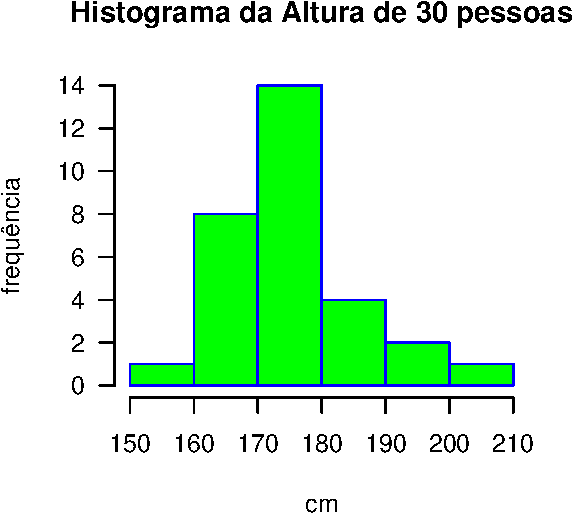
\includegraphics{EstatEcon_files/figure-latex/histograma12-1.pdf}

O pacote \textbf{ggplot2} gera gráficos e histogramas melhor elaborados.

\textbf{Obtendo o histograma usando uma forma alternativa}

Agrupando essas pessoas em \textbf{classes} de 10 cm temos:

\begin{longtable}[]{@{}cc@{}}
\toprule
classes & frequência\tabularnewline
\midrule
\endhead
{[}150 ; 160{[} & 1\tabularnewline
{[}160 ; 170{[} & 8\tabularnewline
{[}170 ; 180{[} & 14\tabularnewline
{[}180 ; 190{[} & 4\tabularnewline
{[}190 ; 200{[} & 2\tabularnewline
{[}200 ; 210{[} & 1\tabularnewline
\bottomrule
\end{longtable}

Fazendo isso no R:

\begin{Shaded}
\begin{Highlighting}[]
\NormalTok{nobs <-}\StringTok{ }\KeywordTok{c}\NormalTok{(}\DecValTok{1}\OperatorTok{:}\DecValTok{30}\NormalTok{)}
\NormalTok{dataX <-}\StringTok{ }\KeywordTok{as.data.frame}\NormalTok{(}\KeywordTok{cbind}\NormalTok{(nobs, X))}
\CommentTok{# transformando em data frame}
\KeywordTok{tail}\NormalTok{(dataX)}
\end{Highlighting}
\end{Shaded}

\begin{verbatim}
##    nobs   X
## 25   25 181
## 26   26 183
## 27   27 185
## 28   28 190
## 29   29 194
## 30   30 201
\end{verbatim}

\begin{Shaded}
\begin{Highlighting}[]
\CommentTok{# mostrando as seis últimas observações}
\NormalTok{quebras <-}\StringTok{ }\KeywordTok{seq}\NormalTok{(}\DecValTok{150}\NormalTok{, }\DecValTok{210}\NormalTok{, }\DataTypeTok{by =} \DecValTok{10}\NormalTok{)}
\CommentTok{# definindo os intervalos}
\NormalTok{quebras}
\end{Highlighting}
\end{Shaded}

\begin{verbatim}
## [1] 150 160 170 180 190 200 210
\end{verbatim}

\begin{Shaded}
\begin{Highlighting}[]
\NormalTok{dataX.cut <-}\StringTok{ }\KeywordTok{cut}\NormalTok{(dataX}\OperatorTok{$}\NormalTok{X, quebras, }\DataTypeTok{right =} \OtherTok{FALSE}\NormalTok{)}
\CommentTok{# construindo as classes fechado a esq e aberto a}
\CommentTok{# direita}
\NormalTok{dataX.freq <-}\StringTok{ }\KeywordTok{table}\NormalTok{(dataX.cut)}
\CommentTok{# obtendo a frequência para cada classe.}
\NormalTok{dataXfreq <-}\StringTok{ }\KeywordTok{cbind}\NormalTok{(dataX.freq)}
\CommentTok{# colocando os dados em colunas}
\NormalTok{dataXfreq}
\end{Highlighting}
\end{Shaded}

\begin{verbatim}
##           dataX.freq
## [150,160)          1
## [160,170)          8
## [170,180)         14
## [180,190)          4
## [190,200)          2
## [200,210)          1
\end{verbatim}

\hypertarget{diagrama-de-caixa-boxplot}{%
\subsection{Diagrama de caixa (Boxplot)}\label{diagrama-de-caixa-boxplot}}

O texto sobre o diagrama de caixa foi baseado em \citet{Morettin2013}.

Boxplot ou caixa de bigode também é uma ferramenta da estatística descritva que permite visualizar a dispersão dos valores da variável em análise. O que define o diagrama de caixa são os quartis. A parte inferior e superior da caixa, são respectivamente o primeiro quartil (\(Q_1\)) e o terceiro quartil (\(Q_3\)). A linha que corta da caixa é a mediana ou o segundo quartil (\(Q_2\)). Os bigodes que são as linhas que se estendem a partir da caixa, são calculado com base na amplitude interquartil (\(AIQ\)). A amplitude interquartil é a diferença entre os valores do terceiro e do primeiro quartis. Ou seja,

\begin{equation*}
  AIQ = Q_3 - Q_1
\end{equation*}

O bigode inferior denominado \(LI\) é calculado subtraindo \(1,5\times AIQ\) do valor do primeiro quartil \(Q_1\). Ou seja,

\begin{equation*}
  LI = Q_1 - 1,5 \times AIQ
\end{equation*}

O bigode superior, denominado \(LS\), é calculado somando \(1,5\times AIQ\) ao valor da terceiro quartil \(Q_3\). Ou seja,

\begin{equation*}
  LS = Q_1 + 1,5 \times AIQ
\end{equation*}

Os valores que forem menor que o \(LI\) ou maior que o \(LS\) são denominados valores discrepantes oui \emph{outliers}. Os valores discrepantes, quando existentes, são colocados separadamente no diagrama de caixa mantendo a distancia relativa do limite inferior ou do limite superior.

Toma-se o mesmo exemplo da altura de 30 pessoas para apresentar o boxplot.

O código seria:

\begin{Shaded}
\begin{Highlighting}[]
\KeywordTok{boxplot}\NormalTok{(X, }\DataTypeTok{data =}\NormalTok{ dataX, }\DataTypeTok{main =} \StringTok{"Diagrama de Caixa"}\NormalTok{, }
    \DataTypeTok{ylab =} \StringTok{"cm"}\NormalTok{, }\DataTypeTok{xlab =} \StringTok{"altura de 30 pessoas"}\NormalTok{)}
\end{Highlighting}
\end{Shaded}

e o resultado segue abaixo.

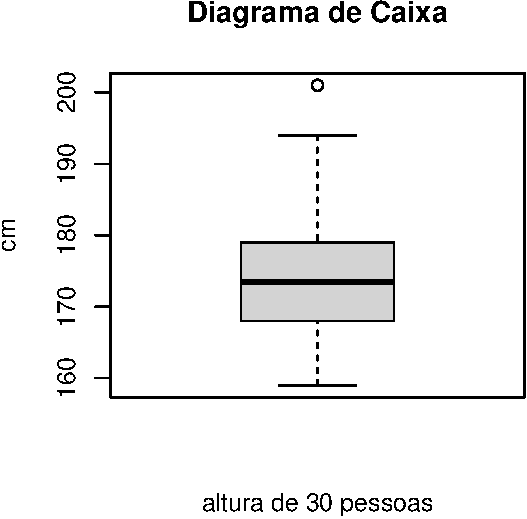
\includegraphics{EstatEcon_files/figure-latex/diagrama de caixa12-1.pdf}

\hypertarget{medidas-de-relauxe7uxe3o-linear-entre-duas-variuxe1veis}{%
\section{Medidas de relação linear entre duas variáveis}\label{medidas-de-relauxe7uxe3o-linear-entre-duas-variuxe1veis}}

Este assunto tem como base o material de \citet{Sartoris2013}.

Parece um pouco estranho incluir esse tópico logo depois das medidas de dispersão. Mas a variância é um caso especial da covariância que é a primeira medida de relação linear entre duas variáveis.

O coeficiente de correlação utiliza a covariância e o desvio padrão para resolver o problema de interpretação do resultado da covariância.

\hypertarget{covariuxe2ncia}{%
\subsection{Covariância}\label{covariuxe2ncia}}

pode ser estendida como uma \emph{variância conjunta} entre duas variáveis. Ou seja,
\begin{equation*}
  cov(X,Y) = \frac{1}{n}\sum_{i=1}^{n}(X_i - \overline{X})(Y_i - \overline{Y})
\end{equation*}

\textbf{Fórmula alternativa da Variância}

Também existe a fórmula alternativa da covariância.

\begin{equation*}
  cov(X,Y) = \frac{1}{n}\sum_{i=1}^{n}X_{i}Y_{i} - \overline{X}\overline{Y}.
\end{equation*}

\textbf{Fórmula alternativa da Covariância}

Em outras palavras

\begin{equation*}
  cov(X,Y) = \text{média dos produtos de X e Y} - \text{produto das médias de X e Y}.
\end{equation*}

\textbf{Covariância no R}

Tomando o exemplo de consumo e renda da tabela 2.11 (Sartoris, 2013, p.42) tem-se

\begin{longtable}[]{@{}cccc@{}}
\toprule
Ano & Consumo(X) & Renda(Y) & (XY)\tabularnewline
\midrule
\endhead
1 & 600 & 1.000 & 600.000\tabularnewline
2 & 700 & 1.100 & 770.000\tabularnewline
3 & 800 & 1.300 & 1.040.000\tabularnewline
4 & 900 & 1.400 & 1.260.000\tabularnewline
\textbf{Somatória} & \textbf{3.000} & \textbf{4.800} & \textbf{3.670.000}\tabularnewline
\textbf{Média} & \textbf{750} & \textbf{1.200} & \textbf{917.500}\tabularnewline
\bottomrule
\end{longtable}

\textbf{Covariância no R}

\begin{Shaded}
\begin{Highlighting}[]
\NormalTok{C1 <-}\StringTok{ }\KeywordTok{c}\NormalTok{(}\DecValTok{600}\NormalTok{, }\DecValTok{700}\NormalTok{, }\DecValTok{800}\NormalTok{, }\DecValTok{900}\NormalTok{)}
\NormalTok{R1 <-}\StringTok{ }\KeywordTok{c}\NormalTok{(}\DecValTok{1000}\NormalTok{, }\DecValTok{1100}\NormalTok{, }\DecValTok{1300}\NormalTok{, }\DecValTok{1400}\NormalTok{)}
\NormalTok{mediaC1 <-}\StringTok{ }\KeywordTok{sum}\NormalTok{(C1)}\OperatorTok{/}\KeywordTok{length}\NormalTok{(C1)}
\NormalTok{mediaR1 <-}\StringTok{ }\KeywordTok{sum}\NormalTok{(R1)}\OperatorTok{/}\KeywordTok{length}\NormalTok{(R1)}
\NormalTok{mediaC1R1 <-}\StringTok{ }\KeywordTok{sum}\NormalTok{(C1 }\OperatorTok{*}\StringTok{ }\NormalTok{R1)}\OperatorTok{/}\KeywordTok{length}\NormalTok{(C1)}
\NormalTok{covC1R1 <-}\StringTok{ }\NormalTok{mediaC1R1 }\OperatorTok{-}\StringTok{ }\NormalTok{mediaC1 }\OperatorTok{*}\StringTok{ }\NormalTok{mediaR1}
\NormalTok{covC1R1}
\end{Highlighting}
\end{Shaded}

\begin{verbatim}
## [1] 17500
\end{verbatim}

\begin{Shaded}
\begin{Highlighting}[]
\KeywordTok{cov}\NormalTok{(C1, R1)}
\end{Highlighting}
\end{Shaded}

\begin{verbatim}
## [1] 23333,33
\end{verbatim}

Note que a função covariância no R é calculada dividindo por \((n-1)\) e não por \(n\).

\hypertarget{coeficiente-de-correlauxe7uxe3o}{%
\subsection{Coeficiente de Correlação}\label{coeficiente-de-correlauxe7uxe3o}}

É obtido dividindo a covariância pelos desvios padrões das variáveis, retirando-se o efeito dos valores de cada variável. Como as unidades das variáveis se cancelam matematicamente, o coeficiente de correlação é um número puro que varia entre -1 e +1. Essa característica o torna mais fácil e claro a sua interpretação. Ou seja,

\begin{equation*}
 corr(X,Y) \cong \rho_{xy} = \frac{cov(X,Y)}{dp(X) \times dp(Y)}
\end{equation*}
onde
\begin{equation*}
  -1 \leq \rho \leq +1
\end{equation*}

Portanto, quando o coeficiente de correlação é igual a zero ou muito próximo a zero, significa que as duas variáveis analisadas não tem relação do tipo linear entre elas. Quando a o coeficiente de correlação é igual a -1 ou próximo de -1, tal fato indica que a existência de uma relação do tipo linear entre as duas vari
áveis analisadas, sendo que as variações ocorrem no setido oposto. Ou seja, quando uma das variáveis aumenta de valor, a outra diminui. Quando o coeficiente de correlação é igual a +1 ou muito próximo de um positivo, tal fato indica que as duas variáveis tem uma relação do tipo linear, sendo que as variações em ambas as variáveis ocorrem no mesmo sentido. Ou seja, quando uma das variáveis aumenta de valor, a outra aumenta também. O que significa o coeficiente de correlação ser: i) exatamente igual a zero; ii) ser exatamente igual a -1 e; exatamente igual a +1?

\textbf{Correlação no R}

\begin{Shaded}
\begin{Highlighting}[]
\NormalTok{medC1 <-}\StringTok{ }\KeywordTok{sum}\NormalTok{(C1)}\OperatorTok{/}\KeywordTok{length}\NormalTok{(C1)}
\NormalTok{medR1 <-}\StringTok{ }\KeywordTok{sum}\NormalTok{(R1)}\OperatorTok{/}\KeywordTok{length}\NormalTok{(R1)}
\NormalTok{varC1 <-}\StringTok{ }\NormalTok{(}\KeywordTok{sum}\NormalTok{((C1 }\OperatorTok{-}\StringTok{ }\NormalTok{medC1)}\OperatorTok{^}\DecValTok{2}\NormalTok{))}\OperatorTok{/}\KeywordTok{length}\NormalTok{(C1)}
\NormalTok{varC1}
\end{Highlighting}
\end{Shaded}

\begin{verbatim}
## [1] 12500
\end{verbatim}

\begin{Shaded}
\begin{Highlighting}[]
\NormalTok{varR1 <-}\StringTok{ }\NormalTok{(}\KeywordTok{sum}\NormalTok{((R1 }\OperatorTok{-}\StringTok{ }\NormalTok{medR1)}\OperatorTok{^}\DecValTok{2}\NormalTok{))}\OperatorTok{/}\KeywordTok{length}\NormalTok{(R1)}
\NormalTok{varR1}
\end{Highlighting}
\end{Shaded}

\begin{verbatim}
## [1] 25000
\end{verbatim}

\begin{Shaded}
\begin{Highlighting}[]
\NormalTok{dpC1 <-}\StringTok{ }\KeywordTok{abs}\NormalTok{(}\KeywordTok{sqrt}\NormalTok{(varC1))}
\NormalTok{dpR1 <-}\StringTok{ }\KeywordTok{abs}\NormalTok{(}\KeywordTok{sqrt}\NormalTok{(varR1))}
\NormalTok{corrC1R1 <-}\StringTok{ }\KeywordTok{round}\NormalTok{(covC1R1}\OperatorTok{/}\NormalTok{(dpC1 }\OperatorTok{*}\StringTok{ }\NormalTok{dpR1), }\DecValTok{4}\NormalTok{)}
\NormalTok{corrC1R1}
\end{Highlighting}
\end{Shaded}

\begin{verbatim}
## [1] 0,9899
\end{verbatim}

Ou simplesmente

\begin{Shaded}
\begin{Highlighting}[]
\KeywordTok{round}\NormalTok{(}\KeywordTok{cor}\NormalTok{(C1, R1), }\DecValTok{4}\NormalTok{)}
\end{Highlighting}
\end{Shaded}

\begin{verbatim}
## [1] 0,9899
\end{verbatim}

\hypertarget{medidas-de-desigualdade}{%
\chapter{Medidas de desigualdade}\label{medidas-de-desigualdade}}

O assunto sobre medidas de desigualdade está baseada na sua totalidade no capítulo 17 de \citet{Hoffmann2006}

\hypertarget{pruxedncipio-de-pigou-dalton}{%
\section{Príncipio de Pigou-Dalton}\label{pruxedncipio-de-pigou-dalton}}

A condição de Pigou-Dalton define que as medidas de desigualdades devem ter seus valores aumentados quando há transferência regressivas de renda.
Para entender a condicção de Pigou-Dalton, considere uma população com apenas duas pessoas cujas rendas são \(X_1\) e \(X_2\). Então, \(\mu = \frac{X_1 + X_2}{2}\). No caso de perfeita igualdade, \(X_1 = X_2 = \mu\). No caso de uma distribuição com \(X_1 \neq X_2\), uma transferência de renda do mais pobre para o mais rico, mantendo a renda média constante, aumenta o grau de desigualdade.

\hypertarget{transferuxeancia-regressiva}{%
\section{Transferência Regressiva}\label{transferuxeancia-regressiva}}

Essa tranferência de renda do mais pobre para o mais rico, mantida a renda média constante, é denominada como \textbf{transferência regressiva} de renda. Portanto, uma \textbf{transferência progressiva} é a transferência de renda do mais rico para o mais pobre.

\hypertarget{curva-de-lorenz}{%
\section{Curva de Lorenz}\label{curva-de-lorenz}}

\begin{longtable}[]{@{}rcccc@{}}
\caption{\label{tab:pessoasocupadas} Distribuição de pessoas ocupadas conforme renda obtida na atividade exercida no Brasil, de acordo com a PNAD 2003}\tabularnewline
\toprule
\begin{minipage}[b]{0.11\columnwidth}\raggedleft
estrato\strut
\end{minipage} & \begin{minipage}[b]{0.19\columnwidth}\centering
\% no estrato
da população
(\%)\strut
\end{minipage} & \begin{minipage}[b]{0.17\columnwidth}\centering
\% no estrato
da renda
(\%)\strut
\end{minipage} & \begin{minipage}[b]{0.17\columnwidth}\centering
\% acumulada
da população
(100\(p\))\strut
\end{minipage} & \begin{minipage}[b]{0.21\columnwidth}\centering
\% acumulada
da renda
(100\(\Phi\))\strut
\end{minipage}\tabularnewline
\midrule
\endfirsthead
\toprule
\begin{minipage}[b]{0.11\columnwidth}\raggedleft
estrato\strut
\end{minipage} & \begin{minipage}[b]{0.19\columnwidth}\centering
\% no estrato
da população
(\%)\strut
\end{minipage} & \begin{minipage}[b]{0.17\columnwidth}\centering
\% no estrato
da renda
(\%)\strut
\end{minipage} & \begin{minipage}[b]{0.17\columnwidth}\centering
\% acumulada
da população
(100\(p\))\strut
\end{minipage} & \begin{minipage}[b]{0.21\columnwidth}\centering
\% acumulada
da renda
(100\(\Phi\))\strut
\end{minipage}\tabularnewline
\midrule
\endhead
\begin{minipage}[t]{0.11\columnwidth}\raggedleft
I\strut
\end{minipage} & \begin{minipage}[t]{0.19\columnwidth}\centering
30\strut
\end{minipage} & \begin{minipage}[t]{0.17\columnwidth}\centering
7\strut
\end{minipage} & \begin{minipage}[t]{0.17\columnwidth}\centering
30\strut
\end{minipage} & \begin{minipage}[t]{0.21\columnwidth}\centering
7\strut
\end{minipage}\tabularnewline
\begin{minipage}[t]{0.11\columnwidth}\raggedleft
II\strut
\end{minipage} & \begin{minipage}[t]{0.19\columnwidth}\centering
20\strut
\end{minipage} & \begin{minipage}[t]{0.17\columnwidth}\centering
9\strut
\end{minipage} & \begin{minipage}[t]{0.17\columnwidth}\centering
50\strut
\end{minipage} & \begin{minipage}[t]{0.21\columnwidth}\centering
16\strut
\end{minipage}\tabularnewline
\begin{minipage}[t]{0.11\columnwidth}\raggedleft
III\strut
\end{minipage} & \begin{minipage}[t]{0.19\columnwidth}\centering
20\strut
\end{minipage} & \begin{minipage}[t]{0.17\columnwidth}\centering
13\strut
\end{minipage} & \begin{minipage}[t]{0.17\columnwidth}\centering
70\strut
\end{minipage} & \begin{minipage}[t]{0.21\columnwidth}\centering
29\strut
\end{minipage}\tabularnewline
\begin{minipage}[t]{0.11\columnwidth}\raggedleft
IV\strut
\end{minipage} & \begin{minipage}[t]{0.19\columnwidth}\centering
10\strut
\end{minipage} & \begin{minipage}[t]{0.17\columnwidth}\centering
10\strut
\end{minipage} & \begin{minipage}[t]{0.17\columnwidth}\centering
80\strut
\end{minipage} & \begin{minipage}[t]{0.21\columnwidth}\centering
39\strut
\end{minipage}\tabularnewline
\begin{minipage}[t]{0.11\columnwidth}\raggedleft
V\strut
\end{minipage} & \begin{minipage}[t]{0.19\columnwidth}\centering
10\strut
\end{minipage} & \begin{minipage}[t]{0.17\columnwidth}\centering
16\strut
\end{minipage} & \begin{minipage}[t]{0.17\columnwidth}\centering
90\strut
\end{minipage} & \begin{minipage}[t]{0.21\columnwidth}\centering
55\strut
\end{minipage}\tabularnewline
\begin{minipage}[t]{0.11\columnwidth}\raggedleft
VI\strut
\end{minipage} & \begin{minipage}[t]{0.19\columnwidth}\centering
5\strut
\end{minipage} & \begin{minipage}[t]{0.17\columnwidth}\centering
13\strut
\end{minipage} & \begin{minipage}[t]{0.17\columnwidth}\centering
95\strut
\end{minipage} & \begin{minipage}[t]{0.21\columnwidth}\centering
68\strut
\end{minipage}\tabularnewline
\begin{minipage}[t]{0.11\columnwidth}\raggedleft
VII\strut
\end{minipage} & \begin{minipage}[t]{0.19\columnwidth}\centering
4\strut
\end{minipage} & \begin{minipage}[t]{0.17\columnwidth}\centering
19\strut
\end{minipage} & \begin{minipage}[t]{0.17\columnwidth}\centering
99\strut
\end{minipage} & \begin{minipage}[t]{0.21\columnwidth}\centering
87\strut
\end{minipage}\tabularnewline
\begin{minipage}[t]{0.11\columnwidth}\raggedleft
VIII\strut
\end{minipage} & \begin{minipage}[t]{0.19\columnwidth}\centering
1\strut
\end{minipage} & \begin{minipage}[t]{0.17\columnwidth}\centering
13\strut
\end{minipage} & \begin{minipage}[t]{0.17\columnwidth}\centering
100\strut
\end{minipage} & \begin{minipage}[t]{0.21\columnwidth}\centering
100\strut
\end{minipage}\tabularnewline
\bottomrule
\end{longtable}

Considere os dados da tabela \ref{tab:pessoasocupadas}. Na coluna de porcentagem acumulada podemos observar que 70\% da população possui 29\% da renda. Os percentuais acumlados da população \(p\) e da renda \(\Phi\) formam um plano cartesinao \((p,\Phi)\) originando a Cuirva de Lorenz.

\begin{Shaded}
\begin{Highlighting}[]
\KeywordTok{library}\NormalTok{(ineq)}
\CommentTok{# usando os valores do exemplo em porcentagem mesmo}
\NormalTok{p <-}\StringTok{ }\KeywordTok{c}\NormalTok{(}\DecValTok{30}\NormalTok{, }\DecValTok{20}\NormalTok{, }\DecValTok{20}\NormalTok{, }\DecValTok{10}\NormalTok{, }\DecValTok{10}\NormalTok{, }\DecValTok{5}\NormalTok{, }\DecValTok{4}\NormalTok{, }\DecValTok{1}\NormalTok{)}
\NormalTok{r <-}\StringTok{ }\KeywordTok{c}\NormalTok{(}\DecValTok{7}\NormalTok{, }\DecValTok{9}\NormalTok{, }\DecValTok{13}\NormalTok{, }\DecValTok{10}\NormalTok{, }\DecValTok{16}\NormalTok{, }\DecValTok{13}\NormalTok{, }\DecValTok{19}\NormalTok{, }\DecValTok{13}\NormalTok{)}

\CommentTok{# calcula o mínimo da curva de Lorenz}
\NormalTok{Lcmin <-}\StringTok{ }\KeywordTok{Lc}\NormalTok{(r, }\DataTypeTok{n =}\NormalTok{ p)}
\CommentTok{# Desenha a curva de Lorenz em um gráfico}
\KeywordTok{plot}\NormalTok{(Lcmin)}
\end{Highlighting}
\end{Shaded}

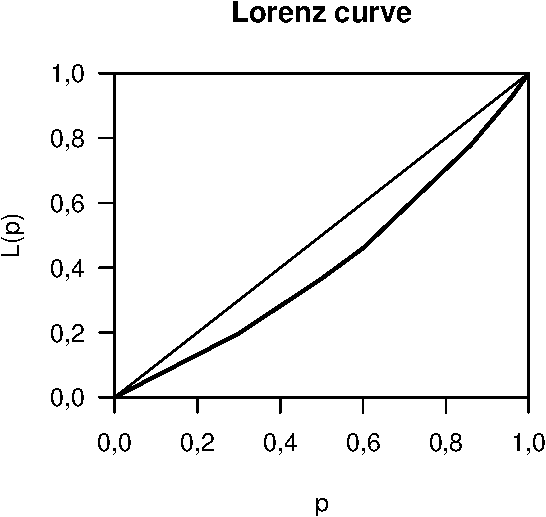
\includegraphics{EstatEcon_files/figure-latex/CurvaLorenzR-1.pdf}
Considerando a curva de Lorenz, figura \ref{fig:CurvaLorenz}, que é basicamente a obtida pelo R, figura \ref{fig:CurvaLorenzR}, mas com algumas indicações, é possível obter algumas definições.

\begin{Shaded}
\begin{Highlighting}[]
\NormalTok{knitr}\OperatorTok{::}\KeywordTok{include_graphics}\NormalTok{(}\StringTok{"lorenz3.png"}\NormalTok{)}
\end{Highlighting}
\end{Shaded}

\begin{figure}

{\centering 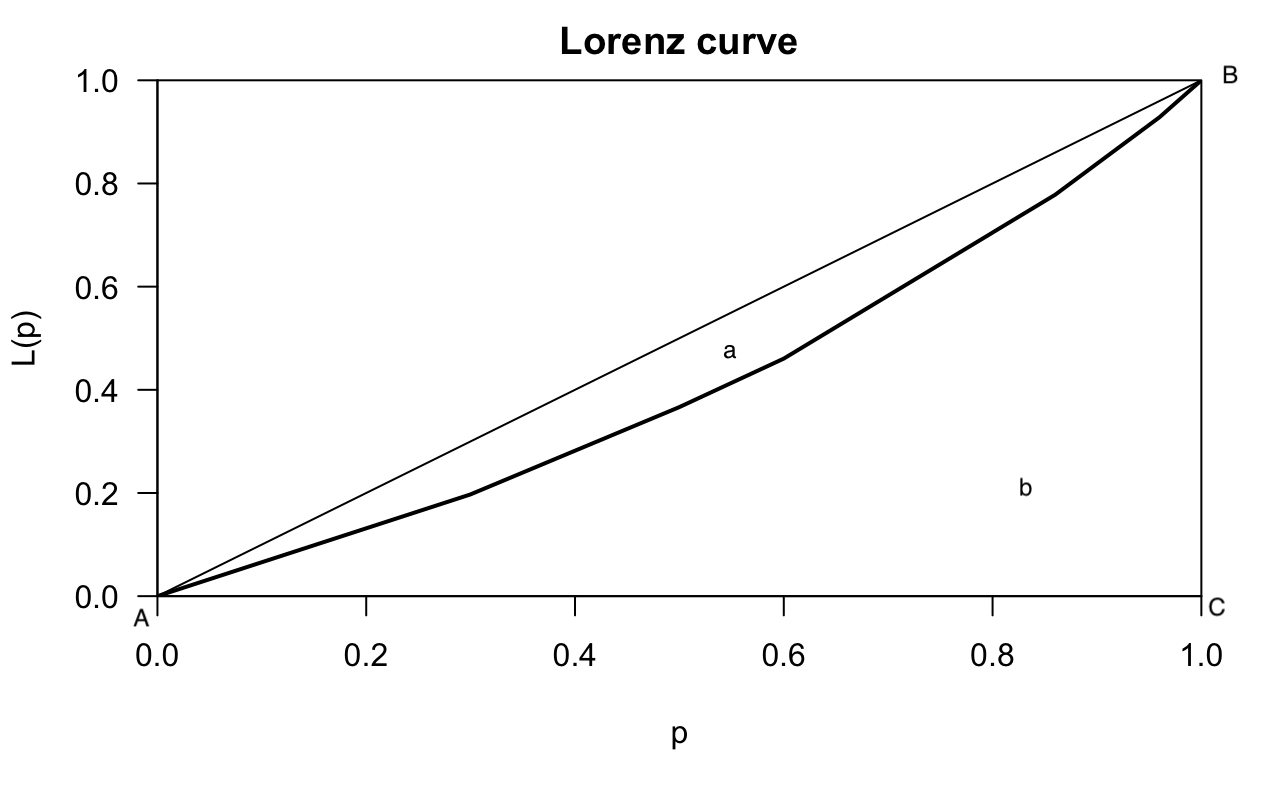
\includegraphics[width=1\linewidth]{lorenz3} 

}

\caption{A curva de Lorenz com algumas indicações}\label{fig:CurvaLorenz}
\end{figure}

A área que corresponde a letra \(a\) é denominada área de desigualdade. o seguimento de retas \(\overline{AB}\) é chamado de \emph{linha de perfeita igualdade} onde \(p=\Phi\) e a área de de desigualdade é zero.

Analisando o casos de máxima desigualdade:

\begin{itemize}
\tightlist
\item
  excluindo-se o fato de renda negativa, considere que apenas um de \(n\) indíviduos receba toda a renda e os demais \(n-1\) indivíduos recebam zero de renda.
\item
  Neste caso a pocentagem de renda é zero até o ponto \(\dfrac{n-1}{n}\) no eixo horizontal, tornando-se \(\Phi = 1\) ao se incluir o último indíviduo.
\item
  Neste caso, a Curva de Lorenz é dada pela poligonal \(\widehat{ABC}\) e a área de desigualdade máxima é o triângulo \(ABC\).
\end{itemize}

\hypertarget{uxedndice-gini}{%
\section{Índice Gini}\label{uxedndice-gini}}

Considere os dados da tabela \ref{tab:pessoasocupadas}. Seja \(p\) o valor da proporção acumulada da população até certo estrato e seja \(\Phi\) o valor da correspondente proporção acumulada da renda. Os pares de valores \((p,\Phi)\), para os diversos estratos, definem pontos em um sistema de eixos cartesianos como aparece na figura \ref{fig:CurvaLorenz}. Estes pontos estão sobre a curva de Lonrez, que mostra como a porporção acumulada da renda \((\Phi)\) varia em função da proporção acumulada da população \((p)\), com as pessoas ordenadas de acordo com valores crescentes da renda. A área correspondente a \(a\) que está entre a reta AB e a curva de Lorenz na figura \ref{fig:CurvaLorenz}, é denominada \textbf{área de desigualdade}.

Para entender como ocorre a variação desta área de desigualdade, a área \(a\), primeiro considere uma situação de distribuição de renda com perfeita igualdade, ou seja, uma população em que todos recebem a mesma renda.Nesta situação, a uma população \(p\) da população corresponde uma igual proporção \(\Phi\) da renda total, ou seja, \(\Phi = p\). Portanto, a curva de Lorenz dessa distribuição coincide com a reta AB da figura \ref{fig:CurvaLorenz}, denominado, por isso, de \textbf{linha de perfeita igualdade}. Neste caso a área de desigualdade é igual a zero.

Considere agora uma outra situação, uma distribuição de renda com o máximo de desigualdade. Considerando que \textbf{não} existe a possibilidade de renda negativa, esse seria o caso de uma população com \(n\) pessoas, em que uma delas recebe toda a renda e as \(n-1\) restante receba zero de renda. Nesta situação, a proporção acumulada da renda é igual a zero até o ponto do eixo horizontal (abcissa) \(\frac{(n-1)}{n}\), tornando-se \(\Phi = 1\) quando se se inclui a pessoa que recebe toda a renda. Neste caso, a curva de Lorenz passa a ser a poligonal ABC da figura \ref{fig:CurvaLorenz}. Que é numericamente igual a 0,5 (Por quê?).

Por definição, o \textbf{índice de Gini (G)} é uma relação entre a área de desigualdade, indicada por \(a\) que passar a ser denominada de \(\alpha\), e a área do triângulo ABC que é numericamente igual a 0,5, ou seja,

\[
G = \dfrac{\alpha}{0,5} = 2\alpha
\label{eq:Gini}
\]

A fórmula \eqref{eq:Gini} é uma das fórmulas de Gini que tem utilidade do ponto de vista teórico.Uma vez que

\[
0 \leq \alpha \leq 0,5
\]

tem se que

\[
0 \leq G \leq 1
\]

Ou seja de que o índice de Gini varia entre entre zero, ausência de desigualdade, e um, máxima desigualdade.Adicionalmente, o índice de Gini é um número adimensional.

Uma fórmula alternativa e mais prática do ponto de vista do cálculo do índice de Gini pode ser obitda considerando-se uma distribuição discreta.

Seja uma variável aleatória discreta \(X_i\) para \(i=1,\ldots,n\), cujos valores estão em ordem crescente

\[
X_1\leq X_2 \leq \ldots \leq X_{n-1} \leq X_n
\]
admitindo-se que os n valores são igualmente prováveis.

a proporção acumulada do número de elementos,m até o i-ésimo elemento, é

\[
p_i = \dfrac{i}{n},~\text{para}~i =1,\ldots, n
\label{eq:ProporcaoDaPopulacao}
\]

A correspondente proporção acumulada de \(X\), até o i-ésimo elemento é

\[
\Phi_i = \dfrac{\sum_{j=1}^{i}X_j}{\sum_{j=1}^{n}X_j} = \dfrac{1}{n\mu}\sum_{j=1}^{i}X_j
\label{eq:ProporcaoDaRendaAcumulada}
\]
onde
\[
\mu = \dfrac{1}{n}\sum_{j=1}^{n}X_j
\]
Se \(X\) representa a renda individual e se \(X_j < X_{j+1}\), \(\Phi_i\) representa a fração da renda total apropriada pelas pessoas com renda inferior ou igual a \(X_i\). As expressões \eqref{eq:ProporcaoDaPopulacao} e \eqref{eq:ProporcaoDaRendaAcumulada} definem as coordenadas \((p_i,\Phi_i)\) com \(i=1,\ldots, n\) de \(n\) pontos da curva de Lorenz. A rigor não existe, nesse caso, uma curva, mas uma poligonal cujos vértices são a origemdos exios e os pontos de coordenadas \((p_i,\Phi_i)\).

Na sequência é apresentada de forma resumida como se calcula o índice de Gini a partir dos valores de \(X_i\) para \(i = 1,\ldots ,n\) da variável. Na figura \ref{fig:CurvaLorenz} a soma das áreas \(a\) e \(b\) totaliza a área do polígono ABC que numericamente é igual a 0,5.
Portanto, \(a = 0,5 - b\). Ou seja, colocando na notação mais elegante,

\[
\alpha = 0,5 - \beta.
\label{eq:alfa}
\]
Substituindo \eqref{eq:alfa} em \eqref{eq:Gini} obtém-se

\[
G = \dfrac{0,5 - \beta}{0,5} = 1 - 2\beta.
\label{eq:GiniEmTermosDeBeta}
\]
Note que a área abaixo da ``curva'' de Lorenz pode ser representada, de forma aproximada, como a soma das áreas de \(n\) trapézios um do lado do outro. Desta forma, a área \(b\) da figura \ref{fig:CurvaLorenz}, compreendida entre a poligonal de Lorenz e o eixo das abscissas, é obtida somando-se a área dos \(n\) trapézios. Ou seja, a área do i-ésimo trapézio é
\[
S_i = \dfrac{\Phi_{i-1} + \Phi_i}{2}\times \dfrac{1}{n}
\label{eq:AreaDoTrapezioSi}
\]
onde \(\Phi_{i-1}\) é a base menor do i-ésimo trapézio; \(\Phi_i\) é a base maior do i-ésimo trapézio e; \(1/n\) é a altura do trapézio que corresponde a pessoa da população composta por n pessoas.

Note que o valor de \(\Phi_0 = 0\), ou seja, o valor de \(\Phi_{i-1}\) para \(i=1\). Com base na fórmula \eqref{eq:AreaDoTrapezioSi} é possível obter a área corresponde a \(b\) na figura \ref{fig:CurvaLorenz} ou \(\beta\) nas notações matemáticas no texto

\[
\beta = \sum_{i=1}^{n}S_i = \dfrac{1}{2n}\sum_{i=1}^{n}(\Phi_{i-1} + \Phi_i)
\label{eq:AreaDoBeta}
\]
Substituindo \eqref{eq:AreaDoBeta} em \eqref{eq:GiniEmTermosDeBeta}, obtém-se

\[
G = 1 - \dfrac{1}{n}\sum_{i=1}^{n}(\Phi_{i-1} + \Phi_i)
\label{eq:GiniEmTermosDePhi}
\]
Considerando a fórmula \eqref{eq:ProporcaoDaRendaAcumulada} e que \(\Phi_0 = 0\), se obtém o índice de Gini em termos da variável \(X_i\). Ou seja,

\[
G = 1 - \dfrac{1}{n^2\mu}[(2n-1)X_1 + (2n-3)X_2 + \dots + 3X_{n-1} + 1X_n]
\label{eq:GiniEmTermosDeXi}
\]

Na parte sobre Estatística Descritiva foi apresentada a medida de dispersão chamada Diferença Absoluta Média que é dada por

\[
\Delta = \dfrac{1}{n^2}\sum_{i=1}^{n}\sum_{j=1}^{n}|X_i - X_j|
\label{eq:DiferencaAbsolutaMedia}
\]

Trabalhando algebricamente a fórmula \eqref{eq:DiferencaAbsolutaMedia}

\[
\Delta = 2\mu - \dfrac{2}{n^2}[(2n-1)X_1 + (2n-3)X_2 + \dots + 3X_{n-1} + 1X_n]
\label{eq:DiferencaAbsolutaMediaModificada}
\]

Se dividir \eqref{eq:DiferencaAbsolutaMediaModificada} por \(2\mu\) obtém a fórmula do índice de Gini em termos da medida de dispersão Diferença Absoluta Média

\[
G = \dfrac{\Delta}{2\mu}
\label{eq:GiniEmTermosDeDiferencaAbsolutaMedia}
\]

Tratando-se da distribuição da renda em uma população, a relação \eqref{eq:GiniEmTermosDeDiferencaAbsolutaMedia} mostra que o índice de Gini, como medida de do grau de desigualdade, apresenta a vantagem de medir diretamente as diferenças de rendal, levando em consideração diferenças entre as rendas de \textbf{todos} os pares de pessoas.

Como \(\Delta\) é uma medida de dispersão da distribuição, a relação \eqref{eq:GiniEmTermosDeDiferencaAbsolutaMedia} mostra que o índice de Gini é uma medida de dispersão relativa. Assim, o conceito de desigualdade de uma distribuição se confunde com o conceito de dispersão relativa.

Com um desenvolvimento algébrico de \(\Delta\) é possível transformar a fórmula \eqref{eq:GiniEmTermosDeDiferencaAbsolutaMedia} em

\[
G = \dfrac{2}{n^2\mu}\sum_{i=1}^{n} iX_i - \dfrac{1}{n} - 1
\label{eq:GiniFinal}
\]
A relação \eqref{eq:GiniFinal} mostra que, no cálculo do índice de Gini, cada valor de \(X_i\) da variável aparece poderado por \(i\). Ou seja, \(X_i\) aparece poderada pelo respectivo número de ordem na sequência dos valores ordenados.

\textbf{Exemplo numérico}

Para aplicar a fórmula do índice de Gini, utiliza-se os dados apresentados na tabela abaixo, obtidos de \citet{Hoffmann2006}.

\begin{longtable}[]{@{}cccccc@{}}
\caption{\label{tab:DadosdoExemploNumericoParaGini} Valores de \(X_i\), \(p_i\), \(\Phi_i\) e \(\Phi_{i-1} + \Phi_i\) para a população hipotética de 8 elementos}\tabularnewline
\toprule
\begin{minipage}[b]{0.10\columnwidth}\centering
\(i\)\strut
\end{minipage} & \begin{minipage}[b]{0.12\columnwidth}\centering
\(p_i\)\strut
\end{minipage} & \begin{minipage}[b]{0.12\columnwidth}\centering
\(X_i\)\strut
\end{minipage} & \begin{minipage}[b]{0.18\columnwidth}\centering
\(\sum_{j=1}^{n}X_j\)\strut
\end{minipage} & \begin{minipage}[b]{0.09\columnwidth}\centering
\(\Phi_i\)\strut
\end{minipage} & \begin{minipage}[b]{0.20\columnwidth}\centering
\(\Phi_{i-1} + \Phi_i\)\strut
\end{minipage}\tabularnewline
\midrule
\endfirsthead
\toprule
\begin{minipage}[b]{0.10\columnwidth}\centering
\(i\)\strut
\end{minipage} & \begin{minipage}[b]{0.12\columnwidth}\centering
\(p_i\)\strut
\end{minipage} & \begin{minipage}[b]{0.12\columnwidth}\centering
\(X_i\)\strut
\end{minipage} & \begin{minipage}[b]{0.18\columnwidth}\centering
\(\sum_{j=1}^{n}X_j\)\strut
\end{minipage} & \begin{minipage}[b]{0.09\columnwidth}\centering
\(\Phi_i\)\strut
\end{minipage} & \begin{minipage}[b]{0.20\columnwidth}\centering
\(\Phi_{i-1} + \Phi_i\)\strut
\end{minipage}\tabularnewline
\midrule
\endhead
\begin{minipage}[t]{0.10\columnwidth}\centering
1\strut
\end{minipage} & \begin{minipage}[t]{0.12\columnwidth}\centering
0,125\strut
\end{minipage} & \begin{minipage}[t]{0.12\columnwidth}\centering
1\strut
\end{minipage} & \begin{minipage}[t]{0.18\columnwidth}\centering
1\strut
\end{minipage} & \begin{minipage}[t]{0.09\columnwidth}\centering
0,02\strut
\end{minipage} & \begin{minipage}[t]{0.20\columnwidth}\centering
0,02\strut
\end{minipage}\tabularnewline
\begin{minipage}[t]{0.10\columnwidth}\centering
2\strut
\end{minipage} & \begin{minipage}[t]{0.12\columnwidth}\centering
0,250\strut
\end{minipage} & \begin{minipage}[t]{0.12\columnwidth}\centering
1\strut
\end{minipage} & \begin{minipage}[t]{0.18\columnwidth}\centering
2\strut
\end{minipage} & \begin{minipage}[t]{0.09\columnwidth}\centering
0,04\strut
\end{minipage} & \begin{minipage}[t]{0.20\columnwidth}\centering
0,06\strut
\end{minipage}\tabularnewline
\begin{minipage}[t]{0.10\columnwidth}\centering
3\strut
\end{minipage} & \begin{minipage}[t]{0.12\columnwidth}\centering
0,375\strut
\end{minipage} & \begin{minipage}[t]{0.12\columnwidth}\centering
1\strut
\end{minipage} & \begin{minipage}[t]{0.18\columnwidth}\centering
3\strut
\end{minipage} & \begin{minipage}[t]{0.09\columnwidth}\centering
0,06\strut
\end{minipage} & \begin{minipage}[t]{0.20\columnwidth}\centering
0,10\strut
\end{minipage}\tabularnewline
\begin{minipage}[t]{0.10\columnwidth}\centering
4\strut
\end{minipage} & \begin{minipage}[t]{0.12\columnwidth}\centering
0,500\strut
\end{minipage} & \begin{minipage}[t]{0.12\columnwidth}\centering
2\strut
\end{minipage} & \begin{minipage}[t]{0.18\columnwidth}\centering
5\strut
\end{minipage} & \begin{minipage}[t]{0.09\columnwidth}\centering
0,10\strut
\end{minipage} & \begin{minipage}[t]{0.20\columnwidth}\centering
0,16\strut
\end{minipage}\tabularnewline
\begin{minipage}[t]{0.10\columnwidth}\centering
5\strut
\end{minipage} & \begin{minipage}[t]{0.12\columnwidth}\centering
0,625\strut
\end{minipage} & \begin{minipage}[t]{0.12\columnwidth}\centering
4\strut
\end{minipage} & \begin{minipage}[t]{0.18\columnwidth}\centering
9\strut
\end{minipage} & \begin{minipage}[t]{0.09\columnwidth}\centering
0,18\strut
\end{minipage} & \begin{minipage}[t]{0.20\columnwidth}\centering
0,28\strut
\end{minipage}\tabularnewline
\begin{minipage}[t]{0.10\columnwidth}\centering
6\strut
\end{minipage} & \begin{minipage}[t]{0.12\columnwidth}\centering
0,750\strut
\end{minipage} & \begin{minipage}[t]{0.12\columnwidth}\centering
8\strut
\end{minipage} & \begin{minipage}[t]{0.18\columnwidth}\centering
17\strut
\end{minipage} & \begin{minipage}[t]{0.09\columnwidth}\centering
0,34\strut
\end{minipage} & \begin{minipage}[t]{0.20\columnwidth}\centering
0,52\strut
\end{minipage}\tabularnewline
\begin{minipage}[t]{0.10\columnwidth}\centering
7\strut
\end{minipage} & \begin{minipage}[t]{0.12\columnwidth}\centering
0,875\strut
\end{minipage} & \begin{minipage}[t]{0.12\columnwidth}\centering
13\strut
\end{minipage} & \begin{minipage}[t]{0.18\columnwidth}\centering
30\strut
\end{minipage} & \begin{minipage}[t]{0.09\columnwidth}\centering
0,60\strut
\end{minipage} & \begin{minipage}[t]{0.20\columnwidth}\centering
0,94\strut
\end{minipage}\tabularnewline
\begin{minipage}[t]{0.10\columnwidth}\centering
8\strut
\end{minipage} & \begin{minipage}[t]{0.12\columnwidth}\centering
1,000\strut
\end{minipage} & \begin{minipage}[t]{0.12\columnwidth}\centering
20\strut
\end{minipage} & \begin{minipage}[t]{0.18\columnwidth}\centering
50\strut
\end{minipage} & \begin{minipage}[t]{0.09\columnwidth}\centering
1,00\strut
\end{minipage} & \begin{minipage}[t]{0.20\columnwidth}\centering
1,60\strut
\end{minipage}\tabularnewline
\bottomrule
\end{longtable}

Com essas informações é possível calcular o índice de Gini, através de \eqref{eq:GiniEmTermosDePhi}

\[
G = 1 - \dfrac{1}{n}\sum_{i=1}^{n}(\Phi_{i-1} + \Phi_i);
\]

através de \eqref{eq:GiniEmTermosDeDiferencaAbsolutaMedia}

\[
G = \dfrac{\Delta}{2\mu},
\]
onde
\[
\Delta = \dfrac{1}{n^2}\sum_{i=1}^{n}\sum_{j=1}^{n}|X_i - X_j|
\]
e
\[
\mu = \sum_{i=1}^{n}X_i;
\]
e através de \eqref{eq:GiniFinal}

\[
G = \dfrac{2}{n^2\mu}\sum_{i=1}^{n} iX_i - \dfrac{1}{n} - 1
\]
Usando \eqref{eq:GiniEmTermosDePhi}, é necessário totalizar a coluna \(\Phi_{i-1} + \Phi_i\) na tabela \ref{tab:DadosdoExemploNumericoParaGini}. Ou seja,

\begin{Shaded}
\begin{Highlighting}[]
\KeywordTok{options}\NormalTok{(}\DataTypeTok{OutDec =} \StringTok{","}\NormalTok{)}
\NormalTok{somaphis <-}\StringTok{ }\KeywordTok{c}\NormalTok{(}\FloatTok{0.02}\NormalTok{, }\FloatTok{0.06}\NormalTok{, }\FloatTok{0.1}\NormalTok{, }\FloatTok{0.16}\NormalTok{, }\FloatTok{0.28}\NormalTok{, }\FloatTok{0.52}\NormalTok{, }\FloatTok{0.94}\NormalTok{, }
    \FloatTok{1.6}\NormalTok{)}
\NormalTok{somasomaphis <-}\StringTok{ }\KeywordTok{sum}\NormalTok{(somaphis)}
\NormalTok{somasomaphis}
\end{Highlighting}
\end{Shaded}

\begin{verbatim}
## [1] 3,68
\end{verbatim}

\[
\sum_{i+1}^{8} (\Phi_{i-1} + \Phi_i) = \text{3,68}
\]

Portanto

\begin{Shaded}
\begin{Highlighting}[]
\NormalTok{giniphis <-}\StringTok{ }\DecValTok{1} \OperatorTok{-}\StringTok{ }\DecValTok{1}\OperatorTok{/}\KeywordTok{length}\NormalTok{(somaphis) }\OperatorTok{*}\StringTok{ }\NormalTok{somasomaphis}
\NormalTok{giniphis}
\end{Highlighting}
\end{Shaded}

\begin{verbatim}
## [1] 0,54
\end{verbatim}

\[
G = 1 - \dfrac{1}{8}\times \text{3,68} = \text{0,54}
\]

Para aplicar a fórmula \eqref{eq:GiniEmTermosDeDiferencaAbsolutaMedia} que é a fórmula do índice de Gini em termos de diferença absoluta média, \(\Delta\), é necessário calcular a diferença absoluta média com base nos dados de \(X_i\) da tabela \ref{tab:DadosdoExemploNumericoParaGini}.

\begin{Shaded}
\begin{Highlighting}[]
\NormalTok{xi <-}\StringTok{ }\KeywordTok{c}\NormalTok{(}\DecValTok{1}\NormalTok{, }\DecValTok{1}\NormalTok{, }\DecValTok{1}\NormalTok{, }\DecValTok{2}\NormalTok{, }\DecValTok{4}\NormalTok{, }\DecValTok{8}\NormalTok{, }\DecValTok{13}\NormalTok{, }\DecValTok{20}\NormalTok{)}

\NormalTok{XC <-}\StringTok{ }\KeywordTok{matrix}\NormalTok{(xi, }\DataTypeTok{nrow =} \KeywordTok{length}\NormalTok{(xi), }\DataTypeTok{ncol =} \KeywordTok{length}\NormalTok{(xi), }
    \DataTypeTok{byrow =} \OtherTok{FALSE}\NormalTok{)}
\NormalTok{XC}
\end{Highlighting}
\end{Shaded}

\begin{verbatim}
##      [,1] [,2] [,3] [,4] [,5] [,6] [,7] [,8]
## [1,]    1    1    1    1    1    1    1    1
## [2,]    1    1    1    1    1    1    1    1
## [3,]    1    1    1    1    1    1    1    1
## [4,]    2    2    2    2    2    2    2    2
## [5,]    4    4    4    4    4    4    4    4
## [6,]    8    8    8    8    8    8    8    8
## [7,]   13   13   13   13   13   13   13   13
## [8,]   20   20   20   20   20   20   20   20
\end{verbatim}

\begin{Shaded}
\begin{Highlighting}[]
\NormalTok{XL <-}\StringTok{ }\KeywordTok{matrix}\NormalTok{(xi, }\DataTypeTok{nrow =} \KeywordTok{length}\NormalTok{(xi), }\DataTypeTok{ncol =} \KeywordTok{length}\NormalTok{(xi), }
    \DataTypeTok{byrow =} \OtherTok{TRUE}\NormalTok{)}
\NormalTok{XL}
\end{Highlighting}
\end{Shaded}

\begin{verbatim}
##      [,1] [,2] [,3] [,4] [,5] [,6] [,7] [,8]
## [1,]    1    1    1    2    4    8   13   20
## [2,]    1    1    1    2    4    8   13   20
## [3,]    1    1    1    2    4    8   13   20
## [4,]    1    1    1    2    4    8   13   20
## [5,]    1    1    1    2    4    8   13   20
## [6,]    1    1    1    2    4    8   13   20
## [7,]    1    1    1    2    4    8   13   20
## [8,]    1    1    1    2    4    8   13   20
\end{verbatim}

\begin{Shaded}
\begin{Highlighting}[]
\NormalTok{DIFX <-}\StringTok{ }\NormalTok{XC }\OperatorTok{-}\StringTok{ }\NormalTok{XL}
\NormalTok{DIFX}
\end{Highlighting}
\end{Shaded}

\begin{verbatim}
##      [,1] [,2] [,3] [,4] [,5] [,6] [,7] [,8]
## [1,]    0    0    0   -1   -3   -7  -12  -19
## [2,]    0    0    0   -1   -3   -7  -12  -19
## [3,]    0    0    0   -1   -3   -7  -12  -19
## [4,]    1    1    1    0   -2   -6  -11  -18
## [5,]    3    3    3    2    0   -4   -9  -16
## [6,]    7    7    7    6    4    0   -5  -12
## [7,]   12   12   12   11    9    5    0   -7
## [8,]   19   19   19   18   16   12    7    0
\end{verbatim}

\begin{Shaded}
\begin{Highlighting}[]
\NormalTok{ABSDIFX <-}\StringTok{ }\KeywordTok{abs}\NormalTok{(DIFX)}
\NormalTok{ABSDIFX}
\end{Highlighting}
\end{Shaded}

\begin{verbatim}
##      [,1] [,2] [,3] [,4] [,5] [,6] [,7] [,8]
## [1,]    0    0    0    1    3    7   12   19
## [2,]    0    0    0    1    3    7   12   19
## [3,]    0    0    0    1    3    7   12   19
## [4,]    1    1    1    0    2    6   11   18
## [5,]    3    3    3    2    0    4    9   16
## [6,]    7    7    7    6    4    0    5   12
## [7,]   12   12   12   11    9    5    0    7
## [8,]   19   19   19   18   16   12    7    0
\end{verbatim}

\begin{Shaded}
\begin{Highlighting}[]
\NormalTok{iota <-}\StringTok{ }\KeywordTok{matrix}\NormalTok{(}\DecValTok{1}\NormalTok{, }\DataTypeTok{nrow =} \KeywordTok{length}\NormalTok{(xi), }\DataTypeTok{ncol =} \DecValTok{1}\NormalTok{, }\DataTypeTok{byrow =} \OtherTok{TRUE}\NormalTok{)}
\NormalTok{iota}
\end{Highlighting}
\end{Shaded}

\begin{verbatim}
##      [,1]
## [1,]    1
## [2,]    1
## [3,]    1
## [4,]    1
## [5,]    1
## [6,]    1
## [7,]    1
## [8,]    1
\end{verbatim}

\begin{Shaded}
\begin{Highlighting}[]
\NormalTok{somacolunaABSDIFX <-}\StringTok{ }\KeywordTok{t}\NormalTok{(iota) }\OperatorTok\StringTok{ }\NormalTok{ABSDIFX}
\NormalTok{somacolunaABSDIFX}
\end{Highlighting}
\end{Shaded}

\begin{verbatim}
##      [,1] [,2] [,3] [,4] [,5] [,6] [,7] [,8]
## [1,]   42   42   42   40   40   48   68  110
\end{verbatim}

\begin{Shaded}
\begin{Highlighting}[]
\NormalTok{somalinhasomacolunaABSDIFX <-}\StringTok{ }\NormalTok{somacolunaABSDIFX }\OperatorTok\StringTok{ }
\StringTok{    }\NormalTok{iota}
\NormalTok{somalinhasomacolunaABSDIFX}
\end{Highlighting}
\end{Shaded}

\begin{verbatim}
##      [,1]
## [1,]  432
\end{verbatim}

\begin{Shaded}
\begin{Highlighting}[]
\NormalTok{obs <-}\StringTok{ }\KeywordTok{length}\NormalTok{(xi)}

\NormalTok{delta <-}\StringTok{ }\NormalTok{obs}\OperatorTok{^}\NormalTok{(}\OperatorTok{-}\DecValTok{2}\NormalTok{) }\OperatorTok{*}\StringTok{ }\NormalTok{somalinhasomacolunaABSDIFX}
\NormalTok{delta}
\end{Highlighting}
\end{Shaded}

\begin{verbatim}
##      [,1]
## [1,] 6,75
\end{verbatim}

Ou seja,

\[
\Delta = \dfrac{1}{n^2}\sum_{i=1}^{n}\sum_{j=1}^{n}|X_i - X_j| = \dfrac{1}{(\text{8})^2} \times \text{432} = \text{6,75}
\]

Com a diferença absoluta média de \(X_i\) devidamente calculada, aplica-se a fórmula \eqref{eq:GiniEmTermosDeDiferencaAbsolutaMedia}

\begin{Shaded}
\begin{Highlighting}[]
\NormalTok{ximedio <-}\StringTok{ }\KeywordTok{sum}\NormalTok{(xi)}\OperatorTok{/}\KeywordTok{length}\NormalTok{(xi)}
\NormalTok{ximedio}
\end{Highlighting}
\end{Shaded}

\begin{verbatim}
## [1] 6,25
\end{verbatim}

\begin{Shaded}
\begin{Highlighting}[]
\NormalTok{ginidelta <-}\StringTok{ }\NormalTok{delta}\OperatorTok{/}\NormalTok{(}\DecValTok{2} \OperatorTok{*}\StringTok{ }\NormalTok{ximedio)}
\NormalTok{ginidelta}
\end{Highlighting}
\end{Shaded}

\begin{verbatim}
##      [,1]
## [1,] 0,54
\end{verbatim}

\[
  G = \dfrac{\Delta}{2\mu} = \dfrac{\text{6,75}}{2 \times \text{6,25}} = \text{0,54}
\]

Para aplicar a fórmula \eqref{eq:GiniFinal} na obtenção do índice de Gini é necessário ponderar cada valor de \(X_i\) pela sua respectiva ordem \(i\) e soma todos os respectivos produtos

\[
  \sum_{i=1}^{n}iX_i.
\]

usando os dados da tabela \ref{tab:DadosdoExemploNumericoParaGini}

\begin{Shaded}
\begin{Highlighting}[]
\NormalTok{is <-}\StringTok{ }\KeywordTok{matrix}\NormalTok{(}\DecValTok{1}\OperatorTok{:}\KeywordTok{length}\NormalTok{(xi), }\DataTypeTok{nrow =} \KeywordTok{length}\NormalTok{(xi), }\DataTypeTok{ncol =} \DecValTok{1}\NormalTok{, }
    \DataTypeTok{byrow =} \OtherTok{TRUE}\NormalTok{)}
\NormalTok{is}
\end{Highlighting}
\end{Shaded}

\begin{verbatim}
##      [,1]
## [1,]    1
## [2,]    2
## [3,]    3
## [4,]    4
## [5,]    5
## [6,]    6
## [7,]    7
## [8,]    8
\end{verbatim}

\begin{Shaded}
\begin{Highlighting}[]
\NormalTok{ixi <-}\StringTok{ }\KeywordTok{t}\NormalTok{(is) }\OperatorTok{*}\StringTok{ }\NormalTok{xi}
\NormalTok{ixi}
\end{Highlighting}
\end{Shaded}

\begin{verbatim}
##      [,1] [,2] [,3] [,4] [,5] [,6] [,7] [,8]
## [1,]    1    2    3    8   20   48   91  160
\end{verbatim}

\begin{Shaded}
\begin{Highlighting}[]
\NormalTok{somaixi <-}\StringTok{ }\KeywordTok{sum}\NormalTok{(ixi)}
\NormalTok{somaixi}
\end{Highlighting}
\end{Shaded}

\begin{verbatim}
## [1] 333
\end{verbatim}

\begin{Shaded}
\begin{Highlighting}[]
\NormalTok{ginifinal <-}\StringTok{ }\DecValTok{2}\OperatorTok{/}\NormalTok{(obs}\OperatorTok{^}\DecValTok{2} \OperatorTok{*}\StringTok{ }\NormalTok{ximedio) }\OperatorTok{*}\StringTok{ }\NormalTok{somaixi }\OperatorTok{-}\StringTok{ }\NormalTok{obs}\OperatorTok{^}\NormalTok{(}\OperatorTok{-}\DecValTok{1}\NormalTok{) }\OperatorTok{-}\StringTok{ }
\StringTok{    }\DecValTok{1}
\NormalTok{ginifinal}
\end{Highlighting}
\end{Shaded}

\begin{verbatim}
## [1] 0,54
\end{verbatim}

obtém

\[
  G = \dfrac{2}{n^2\mu}\sum_{i=1}^{n} iX_i - \dfrac{1}{n} - 1 = \dfrac{2}{\text{8}^2 \times \text{6,25}}\times \text{333} - \dfrac{1}{\text{8}} - 1 = \text{0,54}
\]

\hypertarget{discrepuxe2ncia-muxe1xima}{%
\section{Discrepância Máxima}\label{discrepuxe2ncia-muxe1xima}}

Discrepância Máxima é a maior distância entre entre a linha AB e a curva de Lorenz da figura \ref{fig:CurvaLorenz}. Portanto, a discrepância máxima é a diferença máxima entre a relação da porcentagem acumulada da população e a sua respectiva porcentagem acumulada da renda numa situação de exata igualdade dada pela reta AB e a relação da porcentagem acumulada da população e a sua respectiva porcentagem acumulada da renda numa situação de desigualdade entre as pessoas dessa população que na figura corresponde a poligonal da curva de Lorenz. De acordo com \citet{Hoffmann2006}

\[
  D = p_h - \Phi_h
  \label{eq:DiscrepanciaMaximaDefinicao}
\]

Portanto, o cálculo de \(D\) através de \eqref{eq:DiscrepanciaMaximaDefinicao} depende de \(h\), um número inteiro positivo. Encontrando-se \(i=h\) encontra-se a discrepância máxima \(D\).

Seja uma sequência de valores ordenados em ordem crescente de uma variável discreta \(X_i\)

\[
  X_1 \leq X_2 \leq \ldots \leq X_n
\]

sendo válida pelos menos uma desigualdade.

Para o cálculo da discrepância máxima, é importante entender que a mesma ocorre quando a inclinação do segmento da poligonal da curva de Lorenz passa de uma valor menor que um para um valor maior que um. De acordo com \citet{Hoffmann2006}, a inclinação do segmento da poligonal é dada por

\[
  d_i = \dfrac{X_i}{\mu}
\]

Essa mudança é identificada quando o valor de \(X_i\) ordenada em ordem crescente passa de uma valor menor que a média \(\mu\) para um valor maior que a média \(\mu\), ou seja,

\[
  X_i < \mu~~para~1 \leq i \leq h
\]
e
\[
  X_i \geq \mu~~para~h < i \leq n
\]

Nesaas condições percorre-se a sequência de valores em ordem crescente, o valor de \(p_i - \Phi_i\) aumenta até a inclusão do h-ésimo elemento.que corresponde a \eqref{eq:DiscrepanciaMaximaDefinicao}.

Considerando \eqref{eq:DiscrepanciaMaximaDefinicao}, \eqref{eq:ProporcaoDaPopulacao} e \eqref{eq:ProporcaoDaRendaAcumulada} chaga-se em

\[
  D = \dfrac{h}{n} - \dfrac{1}{n\mu}\sum_{i=1}^{h}X_i
\]
que depois de algumas manobras algébricas torna-se

\[
  D = \dfrac{1}{n\mu}\sum_{i=1}^{h}(\mu - X_i)
\label{eq:DiscrepanciaMaximaEmTermosDeXi}
\]
Na parte de estatística descritiva foi apresentado a medida de dispersão desvio absoluto médio

\[
  \delta = \dfrac{1}{n}\sum_{i=1}^{n}|X_i - \mu|
\]
e considerando que
\[
  \delta = \dfrac{1}{n}\left[ -\sum_{i=1}^{h}\left(X_i - \mu\right) + \sum_{i=h+1}^{n}\left(X_i - \mu\right)\right]
\]
e que
\[
  \sum_{i=h+1}^{n}\left(X_i - \mu\right) = -\sum_{i=1}^{h}\left(X_i - \mu\right).
\]
Portanto
\[
\delta = \dfrac{2}{n}\sum_{i=h+1}^{n}\left(X_i - \mu\right) = \dfrac{2}{n}\sum_{i=1}^{h}\left(\mu - X_i \right).
\label{eq:DesvioAbsolutoMedioEquivalentes}
\]
Comparando \eqref{eq:DesvioAbsolutoMedioEquivalentes} e \eqref{eq:DiscrepanciaMaximaEmTermosDeXi} obtém-se

\[
D = \dfrac{\delta}{2\mu}.
\label{eq:DiscrepanciaMaximaFinal}
\]
Se o Desvio Absoluto Médio, \(\delta\), é uma medida de dispersão da distribuição, a fórmula \eqref{eq:DiscrepanciaMaximaFinal} mostra que discrepância máxima, da mesma forma que o índice de Gini, é uma medida de dispersão relativa.
Retomando o exemplo numérico da tabela \ref{tab:DadosdoExemploNumericoParaGini}, é possível obter o valor da sua discrepância máxima através de \eqref{eq:DiscrepanciaMaximaDefinicao}.

\[
D = p_h - \Phi_h = 0,625 - 0,180 = 0,445.
\]
O mesmo resultado poderia ser obtido através da fórmula \eqref{eq:DiscrepanciaMaximaFinal}. Para isso é necessário calcular o desvio absoluto médio, \(\delta\), para os valores de \(X_i\) do exemplo numérico. Ou seja,

\begin{Shaded}
\begin{Highlighting}[]
\NormalTok{somadesvioabsolutomedioxi <-}\StringTok{ }\KeywordTok{sum}\NormalTok{(}\KeywordTok{abs}\NormalTok{(xi }\OperatorTok{-}\StringTok{ }\NormalTok{ximedio))}
\NormalTok{somadesvioabsolutomedioxi}
\end{Highlighting}
\end{Shaded}

\begin{verbatim}
## [1] 44,5
\end{verbatim}

\begin{Shaded}
\begin{Highlighting}[]
\NormalTok{desvioabsolutomedioxi <-}\StringTok{ }\NormalTok{(}\KeywordTok{length}\NormalTok{(xi))}\OperatorTok{^}\NormalTok{(}\OperatorTok{-}\DecValTok{1}\NormalTok{) }\OperatorTok{*}\StringTok{ }\KeywordTok{sum}\NormalTok{(}\KeywordTok{abs}\NormalTok{(xi }\OperatorTok{-}\StringTok{ }
\StringTok{    }\NormalTok{ximedio))}
\NormalTok{desvioabsolutomedioxi}
\end{Highlighting}
\end{Shaded}

\begin{verbatim}
## [1] 5,5625
\end{verbatim}

\[
\delta = \dfrac{1}{n}\sum_{i=1}^{n}|X_i - \mu| = \dfrac{1}{\text{8}}\times \text{44,5} = \text{5,5625}.
\]
Portanto,

\begin{Shaded}
\begin{Highlighting}[]
\NormalTok{discrepanciamaximaxi <-}\StringTok{ }\NormalTok{desvioabsolutomedioxi}\OperatorTok{/}\NormalTok{(}\DecValTok{2} \OperatorTok{*}\StringTok{ }
\StringTok{    }\NormalTok{ximedio)}
\NormalTok{discrepanciamaximaxi}
\end{Highlighting}
\end{Shaded}

\begin{verbatim}
## [1] 0,445
\end{verbatim}

\[
  D = \dfrac{\delta}{2\mu} = \dfrac{\text{5,5625}}{2 \times \text{6,25}} = \text{0,445}.
\]

\hypertarget{redunduxe2ncia-e-uxedndice-de-theil}{%
\section{Redundância e Índice de Theil}\label{redunduxe2ncia-e-uxedndice-de-theil}}

\hypertarget{teoria-da-informauxe7uxe3o}{%
\subsection{Teoria da Informação}\label{teoria-da-informauxe7uxe3o}}

Para entender melhor as medidas de desigualdades de Theil, é necessário introduzir alguns conceitos da teoria da informação.

Seja \(x\), a probabilidadde de ocorrer o evento \(E\).

\begin{itemize}
\item
  Para \(x=1\), a mensagem \textbf{evento \(E\) ocorreu} não tem nenhum conteúdo informativo.
\item
  Para \(x \rightarrow 0\), ou seja, para valores muito pequenos de \(x\), a mensagem \textbf{evento \(E\) ocorreu} tem alto valor informativo.
\end{itemize}

A segunda situação seria, por exemplo, o caso de uma notícia que nos causas surpresa ou de um \emph{furo} de imprensa. Quando \(x\) tende a zero, o conteúdo informativo da mensagem \textbf{evento \(E\) ocorreu} tende a infinito.

Matematicamente, o conteúdo informativo da mensagem que afirma que determinado evento ocorreu é dado por

\[
  h(x) = \log \dfrac{1}{x} = \log x^{-1} = - \log x
  \label{eq:ConteudoInformativo}
\]

De acordo com \citet{Hoffmann2006}, a escolha da função logarítmica é devido a propriedade de atividade do conteúdo informativo no caso de eventos independentes. Portanto, se \(E_1\) e \(E_2\) são dois eventos independentes com probabilidades \(x_1\) e \(x_2\), respectivamente, a probabilidade de que ambos ocorram é \(x_1x_2\). O conteúdo informativo da mensagem de que ambos os eventos ocorreram é

\[
  h(x_1x_2) = \log \dfrac{1}{x_1x_2} = \log\dfrac{1}{x_1} + \log \dfrac{1}{x_2} = h(x_1) + h(x_2)
\]
Em teoria da informação, normalmente se utiliza logarítmos na base 2 ou logarítmos naturais. Desta forma:

\begin{itemize}
\item
  Logaritmos na base 2: o conteúdo informativo é medido em \textbf{bits}.
\item
  Logaritmos naturais: o conteúdo informativo é medido em \textbf{nits}.
\item
  1 bit = 0,693 nit.
\item
  1 nit = 1,443 bit.
\end{itemize}

Generalizando o conceito de informação, é apresentando, na sequência, como se mede o conteúdo informativo de uma \textbf{mensagem sujeita a erro}, ou \textbf{mensagem incerta}.

Para isso, admita-se que a a probabilidade de chover em um determinado dia, em certo local, estabelecida com base em séries históricas, seja \(x_1 = 0,5\). Nesse caso o conteúdo da informação \textbf{chove} é de

\[
  h(x_1) = \log\dfrac{1}{0,5} =\log 2^1 = 1~\text{bit}
\]
Suponha agora que uma previsão de tempo estabeleceu que iria chover. Suponha, também, que, com base nos resultados anteriores de tais previsões, probabilidade de que realmente shova passa a ser \(y_1 = 0,68\). De acordo com as novas suposições, o conteúdo da informação \textbf{chove} é

\[
  h(y_1) = \log\dfrac{1}{o,68} + 0,5564~\text{bit}
\]

O conteúdo informativo da previsão é

\[
  h(x_1) - h(y_1) = \log\dfrac{1}{x_1} - \log\dfrac{1}{y_1} =  1 - 0,5564 = 0,4436~\text{bit}
\]
ou
\[
  h(x_1) - h(y_1) = \log\dfrac{1}{x_1} - \log\dfrac{1}{y_1} = \log\dfrac{1}{x_1} + \log \left(\dfrac{1}{y_1}\right)^{-1} = \log\dfrac{y_1}{x_1} = \log\left(\dfrac{0,50}{0,68}\right)  = 0,4436~\text{bit}.
\]
Ou seja, o conteúdo informativo \textbf{chove}, com base na probabilidade \(x_i\) nos dados históricos e na probabilidade \(y_i\) do histórico de previsões, é de 0,4436 bit.

Generalizando, o coanteúdo informativo de uma mensagem sujeita a erro ou mensagem incerta, como é o caso da previsão, é dado por

\[
  \log \dfrac{y}{x}
  \label{eq:ConteudoInformativoGeral}
\]
onde

\begin{itemize}
\item
  \(x\) é a probabilidade \emph{ex-ante} ou a probabilidade de que o evento ocorra antes de recebida a mensagem;
\item
  \(y\) é a probabilidade \emph{ex-post} ou a probabilidade de que oevento ocorra uma vez recebida a mensagem.
\end{itemize}

Na sequência é apreseantado o conceito de \emph{entropia}.

\textbf{Entropia de uma distribuição \(H(x)\)}

Seja o universo de \(n\) possíveis eventos \(E_i\), para \(i=1,\ldots ,n\), mutuamente exclusivos aos quais associa-se as probabilidades \(x_i\). Sabe-se que

\[
  \sum_{i}^{n} x_i = 1.
\]

A informação esperada de uma mensagem certa, ou seja, a esperança matemática do conteúdo informativo da mensagem \textbf{ocorreu \(E_i\)}, também denominada entropia da distribuição, é

\[
  H(x) = E[h(x_i)] = \sum_{i=1}^{n} x_i h(x_i) = \sum_{i=1}^{n}x_i \log\dfrac{1}{x_i} = - \sum_{i=1}^{n}x_i \log x_i
  \label{eq:InformacaoEsperadaDeUmaMensagemCerta}
\]

Para o caso particular de \(x_i= 0\), adota-se a definição
\[
 x\log x = 0,~~\text{se}~x = 0
 \label{eq:CasoParticularxiIgualA0}
\]
uma vez que
\[
  \lim_{x\rightarrow 0}(x\log x) = 0
\]
Para \(0 < x_i \leq 1\) se tem

\[
\dfrac{1}{x_i}\geq 1
\]

e

\[
\log \dfrac{1}{x_i} \geq 0.
\]
Conclui-se que
\[
H(x) = \sum_{i=1}^{n} x_i \log \dfrac{1}{x_i} = - \sum_{i=1}^{n} x_i \log x_i \geq 0 
\]

\textbf{Valor mínimo de \(H(x)\)}

O valor mínimo de \(H(x)\) ocorre quando uma das probabilidades é 1 e as demais, consequentemente, são nulas. Nesse caso \(H(x) = 0\). Ou seja, na somatória há um único \(x_i=1\) e o restante \(x_i = 0\). Portanto,

\begin{itemize}
\item
  quando \(x=0\)
  \[
    x \log x = 0
  \]
  de acordo com \eqref{eq:CasoParticularxiIgualA0};
\item
  quando \(x=1\) se tem \(\log 1 = 0\) e também
  \[
    x \log x = 0.
  \]
\end{itemize}

Assim o valor mínimo do valor esperado do conteúdo informativo \(H(x)\) é

\[
H(x) = - \sum_{i=1}^{n}x_i \log x_i = 0
\]

\textbf{Valor Máximo de \(H(x)\)}

Para encontrar o valor máximo de \(H(x)\) sujeito a condição de que \(\sum x_i = 1\), utiliza-se o método do multiplicador de Lagrange, escrevendo a seguinte função

\[
  \max H(x) = -\sum_{i=1}^{n}x_i \log x_i
\]
sujeito a
\[
  \sum_{i=1}^{n} x_i = 1
\]
então
\[
  \mathcal{L} = -\sum_{i=1}^{n}x_i \log x_i - \lambda\left( \sum_{i=1}^{n} x_i  - 1 \right)
  \label{eq:LagrangeanoDeHx}
\]
Igualando a zero as derivadas parciais de \eqref{eq:LagrangeanoDeHx} em relação a \(x_i\) e admitindo-se que se usa os logaritmos naturais, se tem:

\[
  \log x_i = -(1 + \lambda),~~para~i=1,\ldots ,n
\]
sendo que
\[
  x_i = e^{-(1+\lambda)} = \dfrac{1}{e^{(1+\lambda)}}.
\]

Note que \(\lambda\) é constante neste caso.

O valor máximo de \(H(x)\) acontece quando todos os valores de \(x_i\), ou seja, todos as probabilidades são iguais entre si e, portanto, igual a \(\dfrac{1}{n}\). Nesse caso,

\[
  H(x) = \sum_{i=1}^{n} x_i \log \dfrac{1}{x_i} = \sum_{i=1}^{n} \dfrac{1}{n} \log n = n \dfrac{1}{n}\log n = \log n 
\]

Resumindo, o valor esperado da informação ou a entropia da distribuição \(H(x)\) varia entre 0 e \(\log n\). Ou seja,

\[
  0\leq H(x) \leq \log n.
  \label{eq:IntervaloDeVariacaoDeHx}
\]

A entropia da distribuíção é máxima, ou seja, há um máximo de incerteza a respeito do que pode ocorrer, quando todos os possíveis eventos são igualmente prováveis, ou seja, quando há um máximo de \emph{desordem} no sistema.

\textbf{Informação de uma mensagem incerta}

Finalmente é apresentado o conceito de informação de uma mensagem incerta. Dado o universo de \(n\) possíveis eventos \(E_i\), mutuamente exclusivos, com probabilidades \(x_i\), para \(i=1, \ldots, n\), considera-se uma mensagem incerta que poderia ser uma previsão ou uma mensagem duvidosa, que transforma as probabilidades \emph{a priori} \(x_i\) em probabilidade \emph{a posteori} \(y_i\), onde \(y_i\) é a probabilidade de ocorrência do evento \(E_i\) depois de recebido a mensagem. Lembrando
\eqref{eq:ConteudoInformativoGeral}, verifica-se que a esperança matemática do conteúdo informativo da mensagem é

\[
I(y:x) = \sum_{i=1}^{n} y_i \log\dfrac{y_i}{x_i}
\label{eq:InformacaoDeUmaMensagemIncerta}
\]

A definição \eqref{eq:ConteudoInformativo}, do conteúdo informativo de uma mensagem certa, é somente um caso especial de \eqref{eq:InformacaoDeUmaMensagemIncerta}, eem que uma probabilidade \emph{a posteriori} é igual a um e todas as outras são iguais a zero, ou seja, \(y_j = 1\) e \(y_i = 0\) para todo \(i\neq j\).

\hypertarget{uxedndice-t-de-theil}{%
\subsection{Índice T de Theil}\label{uxedndice-t-de-theil}}

Seja uma população com \(n\) pessoas em que cada uma recxebe uma fração não negativa da renda total,

\[
  y_i \geq 0,~~com~i=1,\ldots ,n.
\]
Se a renda média é \(\mu\) e \(X_i\) é a renda i-ésima pessoa,
\[
  y_i = \dfrac{X_i}{n\mu}.
\]
Obviamente,
\[
  \sum_{i=1}^{n} y_i = 1.
\]
Os valores de \(y_i\) tem as mesmas propriedades que as probabilidades \(x_i\) associadas a um universo de eventos \(E_i\) da teoria da informação. Assim sendo, pdoe-se, com base em \eqref{eq:InformacaoEsperadaDeUmaMensagemCerta}, definir a \textbf{entropia} da distribuição de renda considerada como sendo
\[
  H(y) = \sum_{i=1}^{n} y_i \log \dfrac{1}{y_i}.
\]
De acordo com \eqref{eq:IntervaloDeVariacaoDeHx}, se tem

\[
  0\leq H(y) \leq \log n.
\]
Assim é possível definir as duas situações extremas:

\begin{itemize}
\item
  o caso de perfeita igualdade na distribuição da renda,
  \[
    y_i = \dfrac{1}{n}~~para~i=1, \ldots, n,
  \]
  se tem \(H(y) = \log n\);
\item
  o caso de perfeita desigualdade na distribuição de renda,
  \[
    y_i = 1,~~para~i=1, \ldots, n,
  \]
  se tem \(H(y) = 0\).
\end{itemize}

A \textbf{entropia} é, portanto, uma medida do grau de igualdade da distribuição. Mas como o objeto de análise é desigualdade, é ,muito mais interessante uma medida de desigualdade. Para isto basta subtrair a entropia do seu valor próprio máximo, \(\log n\). Essa medida, denominada \textbf{Índice T de Theil} da distribuição é dada por

\[
T = \log n - H(y) = \sum_{i=1}^{n}y_i \log n y_i
\label{eq:IndiceTDeTheil}
\]
Para o cálculo do índice T de Theil, pode-se usar os logarítmos naturais ou os logarítmos na base 2, obtendo-se o valor de T en \emph{nits} ou \emph{bits}, respectivamente. Na prática, utiliza-se mais o logarítmo natural.

Note que

\[
  0 \leq T \leq \log n
  \label{eq:IntervaloDoIndiceTDeTheil}
\]
sendo que:

\begin{itemize}
\item
  \(T = 0\) corresponde ao caso de uma distribuição da renda com perfeita igualdade e;
\item
  \(T = \log n\) corresponde ao caso de uma distribuição da renda com perfeita desigualdade.
\end{itemize}

De \eqref{eq:IndiceTDeTheil} se tem

\[
  T = \sum_{i=1}^{n}y_i \log \dfrac{y_i}{\dfrac{1}{n}}.
\]

Comparando essa equação com \eqref{eq:InformacaoDeUmaMensagemIncerta}, verifica-se que o \textbf{índice T de Theil} corresponde à esperança do valor informativo de uma mensagem incerta, em que as probabilidades \emph{a posteriori} são as frações da renda total \(y_i\) apropriadas pelas pessoas, e as probabilidades \emph{a priori} são iguais a \(1/n\), ou seja, iguais à fração da população correspondente a cada pessoa.

\hypertarget{uxedndice-de-l-de-theil}{%
\subsection{Índice de L de Theil}\label{uxedndice-de-l-de-theil}}

A outra medida de desigualdade proposta por Theil, o \textbf{índice L de Theil}, corresponde à esperança do valor informativo de uma mensagem incerta, em que as probabilidades 8a posteriori* são as frações da população \(1/n\) e as probabilidades \emph{a priori} são as frações da renda \(y_i\). Ou seja,

\[
  L = \sum_{i=1}^{n}\dfrac{1}{n} \log \dfrac{\dfrac{1}{n}}{y_i} = \dfrac{1}{n}\sum_{i=1}^{n} \log \dfrac{1}{ny_i}.
  \label{eq:IndiceLDeTheil}
\]
Verifica-se que o \textbf{índice L de Theil} é igual a zero no caso de pefeita igualdade
\[
  y_i = \dfrac{1}{n}
\]
para todo \(i\).

Basta uma das renda aproximar-se de zero para que o valor de \(L\) tenda a infinito, fazendo que o índice \(L\) seja inútil quando se trata de comparar distribuições de renda que incluem valores nulos.

Uma vantagem importante das medidas de desigualdades de Theil na análise da distribuição de renda ou da riqueza é que, quando os dados podem ser agrupados com base em um critério qualquer, por exemplo regiões, os valores de \(T\) e \(L\) podem ser decompostos em uma medida de desigualdade \textbf{entre} grupos, por exemplo inter-regional, e uma média poderada das medidas de desigualdades \textbf{dentro} de grupos, por exemplo dentro das regiões.

\hypertarget{variuxe2ncia-dos-logaritmos}{%
\section{Variância dos Logaritmos}\label{variuxe2ncia-dos-logaritmos}}

A variância dos logaritmos das rendas é frequentemente utilizada como medida da desigualdade da distribuição da renda em uma população. Para uma população com \(n\) pessoas, em que a renda da \(i\)-ésima pessoas aé indicada por \(X_i\) para \(i=1, \ldots, n\), a variância dos logaritmos das rendas é dada por

\[
V(Z) = \dfrac{1}{n} \sum_{i=1}^{n} \left( Z_i - \overline{Z} \right)^2 
\label{eq:VarianciaDosLogaritmos}
\]
onde
\[
Z_i = \log X_i
\]
e
\[
\overline{Z} = \dfrac{1}{n}\sum_{i=1}^{n} Z_i.
\]
Nota-se que \(V(Z)\) só e definida para \(X_i \geq 0\) para \(i=1, \ldots, n\).

Indicando-se por \(X^*\) a média geométrica dos \(X_i\) , se tem

\[
V(Z) = \dfrac{1}{n} \sum_{i=1}^{n} \left( \log \dfrac{X_i}{X^*} \right)^2
\label{eq:VarianciaDosLogaritmosComMediaGeometrica}
\]

A variância dos logaritmos, da mesmaforma que as medias \(T\) e \(L\) de Theill, é uma medida de desigualdade que, quando os dados podem ser agrupados segundo um critério qualquer, pode ser decomposta em um componente que corresponde à desigualdade entre os grupos e uma média podenrada das variâncias dos logarítmos dentro dos grupos.

\hypertarget{nuxfameros-uxedndices}{%
\chapter{Números-Índices}\label{nuxfameros-uxedndices}}

O conteúdo deste tópico foi elaborado com base no capítulo 16 de \citet{Hoffmann2006} e no capítulo 11 de \citet{Sartoris2013}.

\hypertarget{introduuxe7uxe3o}{%
\section{Introdução}\label{introduuxe7uxe3o}}

Os números-índices, ou simplesmente índices, são proporções estatísticas,
geralmente expressas em porcentagem, idealizadas para comparar as situações de
um conjunto de variáveis em épocas ou localidades diversas.

Para quem vai fazer uso do números-índices na análise de um problema, é
importante saber como são obtidos. Mesmo que não seja necessário calcular um
novo índice, é interessante conhecer os métodos de cálculo, pois isso permite
interpretar melhor os índices publicados e avaliar suas limitações.

\hypertarget{preuxe7os-relativos}{%
\section{Preços Relativos}\label{preuxe7os-relativos}}

O número-índice preços relativos é a relação entre o preço de um produto em determinado período (ano ou mês, geralmente) e o preço no período escolhido como base. Esse índice se destina a acompanhar a evolução do preço de determinado produto. O preço relativo pode ser denominado também de índice relativo de preço ou número-índice simples de preço.

Se \(P_0\) é o preço da mercadoria no período-base e \(P_t\) é o preço em um período \(t\), o preço relativo da mercadoria no ano \(t\) é dado por

\begin{equation}
  I(P_t| P_0) = \frac{P_t}{P_0}.
  \label{eq:IndicePrecoRelativo}
\end{equation}

Usualmente, o valor do índice é dado em porcentagem, calculando-se

\begin{equation}
  I^*(P_t| P_0) = \frac{P_t}{P_0}\cdot 100.
  \label{eq:IndicePrecoRelativoPorcentagem}
\end{equation}

\textbf{Exemplo numérico de índice relativo}

Seja os dados da tabela \ref{tab:DadosPrecosQuantidadesDeTresProdutos2001a2005} abaixo

\begin{longtable}[]{@{}ccccccc@{}}
\caption{\label{tab:DadosPrecosQuantidadesDeTresProdutos2001a2005} dados hipotético de preços e quantidades para três produtos no período de 2001 a 2005}\tabularnewline
\toprule
\begin{minipage}[b]{0.08\columnwidth}\centering
ano\strut
\end{minipage} & \begin{minipage}[b]{0.12\columnwidth}\centering
\(P_{1t}\)\strut
\end{minipage} & \begin{minipage}[b]{0.12\columnwidth}\centering
\(Q_{1t}\)\strut
\end{minipage} & \begin{minipage}[b]{0.12\columnwidth}\centering
\(P_{2t}\)\strut
\end{minipage} & \begin{minipage}[b]{0.12\columnwidth}\centering
\(Q_{2t}\)\strut
\end{minipage} & \begin{minipage}[b]{0.12\columnwidth}\centering
\(P_{3t}\)\strut
\end{minipage} & \begin{minipage}[b]{0.12\columnwidth}\centering
\(Q_{3t}\)\strut
\end{minipage}\tabularnewline
\midrule
\endfirsthead
\toprule
\begin{minipage}[b]{0.08\columnwidth}\centering
ano\strut
\end{minipage} & \begin{minipage}[b]{0.12\columnwidth}\centering
\(P_{1t}\)\strut
\end{minipage} & \begin{minipage}[b]{0.12\columnwidth}\centering
\(Q_{1t}\)\strut
\end{minipage} & \begin{minipage}[b]{0.12\columnwidth}\centering
\(P_{2t}\)\strut
\end{minipage} & \begin{minipage}[b]{0.12\columnwidth}\centering
\(Q_{2t}\)\strut
\end{minipage} & \begin{minipage}[b]{0.12\columnwidth}\centering
\(P_{3t}\)\strut
\end{minipage} & \begin{minipage}[b]{0.12\columnwidth}\centering
\(Q_{3t}\)\strut
\end{minipage}\tabularnewline
\midrule
\endhead
\begin{minipage}[t]{0.08\columnwidth}\centering
2001\strut
\end{minipage} & \begin{minipage}[t]{0.12\columnwidth}\centering
12\strut
\end{minipage} & \begin{minipage}[t]{0.12\columnwidth}\centering
3\strut
\end{minipage} & \begin{minipage}[t]{0.12\columnwidth}\centering
5\strut
\end{minipage} & \begin{minipage}[t]{0.12\columnwidth}\centering
7\strut
\end{minipage} & \begin{minipage}[t]{0.12\columnwidth}\centering
20\strut
\end{minipage} & \begin{minipage}[t]{0.12\columnwidth}\centering
3\strut
\end{minipage}\tabularnewline
\begin{minipage}[t]{0.08\columnwidth}\centering
2002\strut
\end{minipage} & \begin{minipage}[t]{0.12\columnwidth}\centering
15\strut
\end{minipage} & \begin{minipage}[t]{0.12\columnwidth}\centering
4\strut
\end{minipage} & \begin{minipage}[t]{0.12\columnwidth}\centering
10\strut
\end{minipage} & \begin{minipage}[t]{0.12\columnwidth}\centering
9\strut
\end{minipage} & \begin{minipage}[t]{0.12\columnwidth}\centering
25\strut
\end{minipage} & \begin{minipage}[t]{0.12\columnwidth}\centering
4\strut
\end{minipage}\tabularnewline
\begin{minipage}[t]{0.08\columnwidth}\centering
2003\strut
\end{minipage} & \begin{minipage}[t]{0.12\columnwidth}\centering
18\strut
\end{minipage} & \begin{minipage}[t]{0.12\columnwidth}\centering
5\strut
\end{minipage} & \begin{minipage}[t]{0.12\columnwidth}\centering
20\strut
\end{minipage} & \begin{minipage}[t]{0.12\columnwidth}\centering
8\strut
\end{minipage} & \begin{minipage}[t]{0.12\columnwidth}\centering
35\strut
\end{minipage} & \begin{minipage}[t]{0.12\columnwidth}\centering
5\strut
\end{minipage}\tabularnewline
\begin{minipage}[t]{0.08\columnwidth}\centering
2004\strut
\end{minipage} & \begin{minipage}[t]{0.12\columnwidth}\centering
24\strut
\end{minipage} & \begin{minipage}[t]{0.12\columnwidth}\centering
5\strut
\end{minipage} & \begin{minipage}[t]{0.12\columnwidth}\centering
30\strut
\end{minipage} & \begin{minipage}[t]{0.12\columnwidth}\centering
7\strut
\end{minipage} & \begin{minipage}[t]{0.12\columnwidth}\centering
45\strut
\end{minipage} & \begin{minipage}[t]{0.12\columnwidth}\centering
6\strut
\end{minipage}\tabularnewline
\begin{minipage}[t]{0.08\columnwidth}\centering
2005\strut
\end{minipage} & \begin{minipage}[t]{0.12\columnwidth}\centering
30\strut
\end{minipage} & \begin{minipage}[t]{0.12\columnwidth}\centering
6\strut
\end{minipage} & \begin{minipage}[t]{0.12\columnwidth}\centering
60\strut
\end{minipage} & \begin{minipage}[t]{0.12\columnwidth}\centering
6\strut
\end{minipage} & \begin{minipage}[t]{0.12\columnwidth}\centering
50\strut
\end{minipage} & \begin{minipage}[t]{0.12\columnwidth}\centering
5\strut
\end{minipage}\tabularnewline
\bottomrule
\end{longtable}

Fonte: \citet{Hoffmann2006}.

Tomando com base o ano 2002, o preço relativo do produto 1 em 2004, de acordo com
\eqref{eq:IndicePrecoRelativoPorcentagem} é

\begin{equation}
    I*(P_t| P_0) = \frac{24}{15}\cdot 100 = 160.
\end{equation}

Com base na tabela \ref{tab:DadosPrecosQuantidadesDeTresProdutos2001a2005}, os demais preços relativos podem ser calculados, tomando como base o ano de 2002, que são apresentados na tabela \ref{tab:PrecosRelativosDosTresProdutosBase2002}.

\begin{longtable}[]{@{}cccc@{}}
\caption{\label{tab:PrecosRelativosDosTresProdutosBase2002} Preços relativos dos três produtos no período de 2001 a 2005, tomando como base o ano de 2002}\tabularnewline
\toprule
\begin{minipage}[b]{0.09\columnwidth}\centering
ano\strut
\end{minipage} & \begin{minipage}[b]{0.15\columnwidth}\centering
Produto 1\strut
\end{minipage} & \begin{minipage}[b]{0.15\columnwidth}\centering
Produto 2\strut
\end{minipage} & \begin{minipage}[b]{0.16\columnwidth}\centering
Produto 3\strut
\end{minipage}\tabularnewline
\midrule
\endfirsthead
\toprule
\begin{minipage}[b]{0.09\columnwidth}\centering
ano\strut
\end{minipage} & \begin{minipage}[b]{0.15\columnwidth}\centering
Produto 1\strut
\end{minipage} & \begin{minipage}[b]{0.15\columnwidth}\centering
Produto 2\strut
\end{minipage} & \begin{minipage}[b]{0.16\columnwidth}\centering
Produto 3\strut
\end{minipage}\tabularnewline
\midrule
\endhead
\begin{minipage}[t]{0.09\columnwidth}\centering
2001\strut
\end{minipage} & \begin{minipage}[t]{0.15\columnwidth}\centering
80\strut
\end{minipage} & \begin{minipage}[t]{0.15\columnwidth}\centering
50\strut
\end{minipage} & \begin{minipage}[t]{0.16\columnwidth}\centering
80\strut
\end{minipage}\tabularnewline
\begin{minipage}[t]{0.09\columnwidth}\centering
2002\strut
\end{minipage} & \begin{minipage}[t]{0.15\columnwidth}\centering
100\strut
\end{minipage} & \begin{minipage}[t]{0.15\columnwidth}\centering
100\strut
\end{minipage} & \begin{minipage}[t]{0.16\columnwidth}\centering
100\strut
\end{minipage}\tabularnewline
\begin{minipage}[t]{0.09\columnwidth}\centering
2003\strut
\end{minipage} & \begin{minipage}[t]{0.15\columnwidth}\centering
120\strut
\end{minipage} & \begin{minipage}[t]{0.15\columnwidth}\centering
200\strut
\end{minipage} & \begin{minipage}[t]{0.16\columnwidth}\centering
140\strut
\end{minipage}\tabularnewline
\begin{minipage}[t]{0.09\columnwidth}\centering
2004\strut
\end{minipage} & \begin{minipage}[t]{0.15\columnwidth}\centering
160\strut
\end{minipage} & \begin{minipage}[t]{0.15\columnwidth}\centering
300\strut
\end{minipage} & \begin{minipage}[t]{0.16\columnwidth}\centering
180\strut
\end{minipage}\tabularnewline
\begin{minipage}[t]{0.09\columnwidth}\centering
2005\strut
\end{minipage} & \begin{minipage}[t]{0.15\columnwidth}\centering
200\strut
\end{minipage} & \begin{minipage}[t]{0.15\columnwidth}\centering
600\strut
\end{minipage} & \begin{minipage}[t]{0.16\columnwidth}\centering
200\strut
\end{minipage}\tabularnewline
\bottomrule
\end{longtable}

\textbf{Exemplo numérico de preço relativo no R}

Carrega-se os preços dos três produtos e calcula os respectivos preços relativos tendo como base o ano de 2002.

\begin{Shaded}
\begin{Highlighting}[]
\NormalTok{prd1 <-}\StringTok{ }\KeywordTok{c}\NormalTok{(}\DecValTok{12}\NormalTok{, }\DecValTok{15}\NormalTok{, }\DecValTok{18}\NormalTok{, }\DecValTok{24}\NormalTok{, }\DecValTok{30}\NormalTok{)}
\NormalTok{prd2 <-}\StringTok{ }\KeywordTok{c}\NormalTok{(}\DecValTok{5}\NormalTok{, }\DecValTok{10}\NormalTok{, }\DecValTok{20}\NormalTok{, }\DecValTok{30}\NormalTok{, }\DecValTok{60}\NormalTok{)}
\NormalTok{prd3 <-}\StringTok{ }\KeywordTok{c}\NormalTok{(}\DecValTok{20}\NormalTok{, }\DecValTok{25}\NormalTok{, }\DecValTok{35}\NormalTok{, }\DecValTok{45}\NormalTok{, }\DecValTok{50}\NormalTok{)}

\NormalTok{iprprd1 <-}\StringTok{ }\NormalTok{prd1}\OperatorTok{/}\NormalTok{prd1[}\DecValTok{2}\NormalTok{] }\OperatorTok{*}\StringTok{ }\DecValTok{100}
\NormalTok{iprprd2 <-}\StringTok{ }\NormalTok{prd2}\OperatorTok{/}\NormalTok{prd2[}\DecValTok{2}\NormalTok{] }\OperatorTok{*}\StringTok{ }\DecValTok{100}
\NormalTok{iprprd3 <-}\StringTok{ }\NormalTok{prd3}\OperatorTok{/}\NormalTok{prd3[}\DecValTok{2}\NormalTok{] }\OperatorTok{*}\StringTok{ }\DecValTok{100}

\NormalTok{ipr161 <-}\StringTok{ }\KeywordTok{cbind}\NormalTok{(iprprd1, iprprd2, iprprd3)}
\KeywordTok{rownames}\NormalTok{(ipr161) <-}\StringTok{ }\KeywordTok{c}\NormalTok{(}\DecValTok{2001}\NormalTok{, }\DecValTok{2002}\NormalTok{, }\DecValTok{2003}\NormalTok{, }\DecValTok{2004}\NormalTok{, }\DecValTok{2005}\NormalTok{)}

\NormalTok{ipr161}
\end{Highlighting}
\end{Shaded}

\begin{verbatim}
##      iprprd1 iprprd2 iprprd3
## 2001      80      50      80
## 2002     100     100     100
## 2003     120     200     140
## 2004     160     300     180
## 2005     200     600     200
\end{verbatim}

Note que na linha da ano 2002, os três preaços relativos em porcentagem são iguais a 100.

O preço relativo mostra como está evoluindo o preço de cada um dos produtos. Mas quando analisa-se um conjunto de mercadorias, interessa-se em obter um único índice que nos mostre como está evoluindo o nível geral dos preços dessas mercadorias.

\hypertarget{uxedndice-simples-de-preuxe7os-agregados}{%
\section{Índice Simples de Preços Agregados}\label{uxedndice-simples-de-preuxe7os-agregados}}

O índice Simples de Preços Agregados é a relação entre o somatório dos preços das mercadorias no período \(t\) e o somatório dos preços das mercadorias no período escolhido como base.
O índice simples de preços agreagados é também chamado de índice agregativo de preços.
Defini-se que o índice \(i\), variando de 1 a \(n\), indique as \(n\) diferentes mercadorias do conjunto considerado.
Note que \(I_A(\mathbf{p_t}|\mathbf{p_0})\) é o valor do índice agregativo para o vetor ou conjunto de preços \(\mathbf{p_t} = {P_{it},i=1,\ldots, n}\) quando comparado ao vetor de preços do período-base, \(\mathbf{p_0} = {P_{i0},i=1,\ldots, n}\). Ou seja,
\begin{equation}
  I_A(\mathbf{p_t}| \mathbf{p_0}) =
  \frac{\sum_{i=1}^{n}P_{it}}{\sum_{i=1}^{n}P_{i0}},
  \label{eq:IndiceSimplesDePrecosAgregados}
\end{equation}
ou em porcentagem
\begin{equation}
  I_A^*(\mathbf{p_t}| \mathbf{p_0}) =
  \frac{\sum_{i=1}^{n}P_{it}}{\sum_{i=1}^{n}P_{i0}} \cdot 100.
  \label{eq:IndiceSimplesDePrecosAgregadosPorcentagem}
\end{equation}

\textbf{Exemplo numérico do Índice simples de preços agregados}

om base nos dados da tabela \ref{tab:DadosPrecosQuantidadesDeTresProdutos2001a2005}, calcula-se o índice simples de preços agregados para os três produtos em 2004, tomando 2002 como ano-base. De acordo com \eqref{eq:IndiceSimplesDePrecosAgregadosPorcentagem},

\begin{equation}
  I_A^*(\mathbf{p_4}| \mathbf{p_2}) =
  \frac{24 + 30 + 45}{15 + 10 +25} \cdot 100 = 198.
\end{equation}

Analogamente, obtém-se os demais índices que são apresentados na tabela \ref{tab:IndiceSimplesDePrecosAgregadosDeTresProdutosBase2002}.

\begin{longtable}[]{@{}cc@{}}
\caption{\label{tab:IndiceSimplesDePrecosAgregadosDeTresProdutosBase2002} Índice simples de preços agregados dos três produtos no período 2001-2005 tomando como base o ano de 2002}\tabularnewline
\toprule
\begin{minipage}[b]{0.09\columnwidth}\centering
ano\strut
\end{minipage} & \begin{minipage}[b]{0.26\columnwidth}\centering
\(I_A^*(P_t|P_0)\)\strut
\end{minipage}\tabularnewline
\midrule
\endfirsthead
\toprule
\begin{minipage}[b]{0.09\columnwidth}\centering
ano\strut
\end{minipage} & \begin{minipage}[b]{0.26\columnwidth}\centering
\(I_A^*(P_t|P_0)\)\strut
\end{minipage}\tabularnewline
\midrule
\endhead
\begin{minipage}[t]{0.09\columnwidth}\centering
2001\strut
\end{minipage} & \begin{minipage}[t]{0.26\columnwidth}\centering
74\strut
\end{minipage}\tabularnewline
\begin{minipage}[t]{0.09\columnwidth}\centering
2002\strut
\end{minipage} & \begin{minipage}[t]{0.26\columnwidth}\centering
100\strut
\end{minipage}\tabularnewline
\begin{minipage}[t]{0.09\columnwidth}\centering
2003\strut
\end{minipage} & \begin{minipage}[t]{0.26\columnwidth}\centering
146\strut
\end{minipage}\tabularnewline
\begin{minipage}[t]{0.09\columnwidth}\centering
2004\strut
\end{minipage} & \begin{minipage}[t]{0.26\columnwidth}\centering
198\strut
\end{minipage}\tabularnewline
\begin{minipage}[t]{0.09\columnwidth}\centering
2005\strut
\end{minipage} & \begin{minipage}[t]{0.26\columnwidth}\centering
280\strut
\end{minipage}\tabularnewline
\bottomrule
\end{longtable}

A seguir é calculado o Índice simples de preços agregados do exemplo numérico no R.

\textbf{Exemplo numérico do índice simples de preços agregados no R}

\begin{Shaded}
\begin{Highlighting}[]
\NormalTok{p1 <-}\StringTok{ }\KeywordTok{c}\NormalTok{(}\DecValTok{12}\NormalTok{, }\DecValTok{15}\NormalTok{, }\DecValTok{18}\NormalTok{, }\DecValTok{24}\NormalTok{, }\DecValTok{30}\NormalTok{)}
\NormalTok{p2 <-}\StringTok{ }\KeywordTok{c}\NormalTok{(}\DecValTok{5}\NormalTok{, }\DecValTok{10}\NormalTok{, }\DecValTok{20}\NormalTok{, }\DecValTok{30}\NormalTok{, }\DecValTok{60}\NormalTok{)}
\NormalTok{p3 <-}\StringTok{ }\KeywordTok{c}\NormalTok{(}\DecValTok{20}\NormalTok{, }\DecValTok{25}\NormalTok{, }\DecValTok{35}\NormalTok{, }\DecValTok{45}\NormalTok{, }\DecValTok{50}\NormalTok{)}

\NormalTok{p161 <-}\StringTok{ }\KeywordTok{cbind}\NormalTok{(p1, p2, p3)}
\KeywordTok{rownames}\NormalTok{(p161) <-}\StringTok{ }\KeywordTok{c}\NormalTok{(}\DecValTok{2001}\NormalTok{, }\DecValTok{2002}\NormalTok{, }\DecValTok{2003}\NormalTok{, }\DecValTok{2004}\NormalTok{, }\DecValTok{2005}\NormalTok{)}

\NormalTok{IAp1p2 <-}\StringTok{ }\KeywordTok{sum}\NormalTok{(p161[}\DecValTok{1}\NormalTok{, ])}\OperatorTok{/}\KeywordTok{sum}\NormalTok{(p161[}\DecValTok{2}\NormalTok{, ]) }\OperatorTok{*}\StringTok{ }\DecValTok{100}
\NormalTok{IAp2p2 <-}\StringTok{ }\KeywordTok{sum}\NormalTok{(p161[}\DecValTok{2}\NormalTok{, ])}\OperatorTok{/}\KeywordTok{sum}\NormalTok{(p161[}\DecValTok{2}\NormalTok{, ]) }\OperatorTok{*}\StringTok{ }\DecValTok{100}
\NormalTok{IAp3p2 <-}\StringTok{ }\KeywordTok{sum}\NormalTok{(p161[}\DecValTok{3}\NormalTok{, ])}\OperatorTok{/}\KeywordTok{sum}\NormalTok{(p161[}\DecValTok{2}\NormalTok{, ]) }\OperatorTok{*}\StringTok{ }\DecValTok{100}
\NormalTok{IAp4p2 <-}\StringTok{ }\KeywordTok{sum}\NormalTok{(p161[}\DecValTok{4}\NormalTok{, ])}\OperatorTok{/}\KeywordTok{sum}\NormalTok{(p161[}\DecValTok{2}\NormalTok{, ]) }\OperatorTok{*}\StringTok{ }\DecValTok{100}
\NormalTok{IAp5p2 <-}\StringTok{ }\KeywordTok{sum}\NormalTok{(p161[}\DecValTok{5}\NormalTok{, ])}\OperatorTok{/}\KeywordTok{sum}\NormalTok{(p161[}\DecValTok{2}\NormalTok{, ]) }\OperatorTok{*}\StringTok{ }\DecValTok{100}

\NormalTok{ispa161 <-}\StringTok{ }\KeywordTok{rbind}\NormalTok{(IAp1p2, IAp2p2, IAp3p2, IAp4p2, IAp5p2)}
\KeywordTok{colnames}\NormalTok{(ispa161) <-}\StringTok{ }\KeywordTok{c}\NormalTok{(}\StringTok{"ISPA"}\NormalTok{)}

\NormalTok{ispa161}
\end{Highlighting}
\end{Shaded}

\begin{verbatim}
##        ISPA
## IAp1p2   74
## IAp2p2  100
## IAp3p2  146
## IAp4p2  198
## IAp5p2  280
\end{verbatim}

\hypertarget{muxe9dia-aritmuxe9tica-dos-preuxe7os-relativos}{%
\section{Média Aritmética dos Preços Relativos}\label{muxe9dia-aritmuxe9tica-dos-preuxe7os-relativos}}

A Média Aritmétirca dos Preços Relativos é um índice geral de preços que se obtém calculando a média aritmética dos preços relativos, isto é

\begin{equation}
  I_M(\mathbf{p_t}| \mathbf{p_0}) = \frac{1}{n}
  \sum_{i=1}^{n}\frac{P_{it}}{P_{i0}}
  \label{eq:MediaAritmeticaPrecosRelativos}
\end{equation}

ou, em porcentagem,

\begin{equation}
  I_M^*(\mathbf{p_t}| \mathbf{p_0}) = \frac{1}{n}
  \sum_{i=1}^{n}\frac{P_{it}}{P_{i0}} \cdot 100.
  \label{eq:MediaAritmeticaPrecosRelativosPorcentagem}
\end{equation}

Na tabela \ref{tab:IndiceSimplesDePrecosAgregadosDeTresProdutosBase2002} abaixo são apresentados os valores desse índice para os dados da tabela \ref{tab:DadosPrecosQuantidadesDeTresProdutos2001a2005}

\begin{longtable}[]{@{}cc@{}}
\caption{\label{tab:IndiceMediaAritmeticaPrecosRelativosDeTresProdutosBase2002} Índice média aritmética dos preços relativos dos três produtos no período 2001-2005 tomando como base o ano de 2002}\tabularnewline
\toprule
\begin{minipage}[b]{0.09\columnwidth}\centering
ano\strut
\end{minipage} & \begin{minipage}[b]{0.26\columnwidth}\centering
\(I_M^*(P_t|P_0)\)\strut
\end{minipage}\tabularnewline
\midrule
\endfirsthead
\toprule
\begin{minipage}[b]{0.09\columnwidth}\centering
ano\strut
\end{minipage} & \begin{minipage}[b]{0.26\columnwidth}\centering
\(I_M^*(P_t|P_0)\)\strut
\end{minipage}\tabularnewline
\midrule
\endhead
\begin{minipage}[t]{0.09\columnwidth}\centering
2001\strut
\end{minipage} & \begin{minipage}[t]{0.26\columnwidth}\centering
70,0\strut
\end{minipage}\tabularnewline
\begin{minipage}[t]{0.09\columnwidth}\centering
2002\strut
\end{minipage} & \begin{minipage}[t]{0.26\columnwidth}\centering
100,0\strut
\end{minipage}\tabularnewline
\begin{minipage}[t]{0.09\columnwidth}\centering
2003\strut
\end{minipage} & \begin{minipage}[t]{0.26\columnwidth}\centering
153,3\strut
\end{minipage}\tabularnewline
\begin{minipage}[t]{0.09\columnwidth}\centering
2004\strut
\end{minipage} & \begin{minipage}[t]{0.26\columnwidth}\centering
213,3\strut
\end{minipage}\tabularnewline
\begin{minipage}[t]{0.09\columnwidth}\centering
2005\strut
\end{minipage} & \begin{minipage}[t]{0.26\columnwidth}\centering
333,3\strut
\end{minipage}\tabularnewline
\bottomrule
\end{longtable}

Note que os valores da tabela \ref{tab:IndiceMediaAritmeticaPrecosRelativosDeTresProdutosBase2002} é a média aritmética dos preços relativos da tabela \ref{tab:DadosPrecosQuantidadesDeTresProdutos2001a2005} para cada ano.

Para o ano de 2003, por exemplo, foi calculada da seguinte forma:

\[
I_M^{*}(P_{2003}|P_{2002}) = \dfrac{1}{3}\times \left( 120 + 200 +140 \right) = 153,3
\]\\
\textbf{Exemplo numérico da média artimética dos preços realtivos no R}

Como temos calculado o preço relativo para cada um dos três produtos com ano
base 2002, é só calcular a média aritmética para cada ano.

\begin{Shaded}
\begin{Highlighting}[]
\NormalTok{ipr161}
\end{Highlighting}
\end{Shaded}

\begin{verbatim}
##      iprprd1 iprprd2 iprprd3
## 2001      80      50      80
## 2002     100     100     100
## 2003     120     200     140
## 2004     160     300     180
## 2005     200     600     200
\end{verbatim}

\begin{Shaded}
\begin{Highlighting}[]
\NormalTok{maprp1p2 <-}\StringTok{ }\KeywordTok{sum}\NormalTok{(ipr161[}\DecValTok{1}\NormalTok{, ])}\OperatorTok{/}\KeywordTok{length}\NormalTok{(ipr161[}\DecValTok{1}\NormalTok{, ])}
\NormalTok{maprp2p2 <-}\StringTok{ }\KeywordTok{sum}\NormalTok{(ipr161[}\DecValTok{2}\NormalTok{, ])}\OperatorTok{/}\KeywordTok{length}\NormalTok{(ipr161[}\DecValTok{2}\NormalTok{, ])}
\NormalTok{maprp3p2 <-}\StringTok{ }\KeywordTok{sum}\NormalTok{(ipr161[}\DecValTok{3}\NormalTok{, ])}\OperatorTok{/}\KeywordTok{length}\NormalTok{(ipr161[}\DecValTok{3}\NormalTok{, ])}
\NormalTok{maprp4p2 <-}\StringTok{ }\KeywordTok{sum}\NormalTok{(ipr161[}\DecValTok{4}\NormalTok{, ])}\OperatorTok{/}\KeywordTok{length}\NormalTok{(ipr161[}\DecValTok{4}\NormalTok{, ])}
\NormalTok{maprp5p2 <-}\StringTok{ }\KeywordTok{sum}\NormalTok{(ipr161[}\DecValTok{5}\NormalTok{, ])}\OperatorTok{/}\KeywordTok{length}\NormalTok{(ipr161[}\DecValTok{5}\NormalTok{, ])}

\NormalTok{mapr161 <-}\StringTok{ }\KeywordTok{round}\NormalTok{(}\KeywordTok{rbind}\NormalTok{(maprp1p2, maprp2p2, maprp3p2, }
\NormalTok{    maprp4p2, maprp5p2), }\DecValTok{1}\NormalTok{)}
\KeywordTok{colnames}\NormalTok{(mapr161) <-}\StringTok{ }\KeywordTok{c}\NormalTok{(}\StringTok{"MAPR"}\NormalTok{)}

\NormalTok{mapr161}
\end{Highlighting}
\end{Shaded}

\begin{verbatim}
##           MAPR
## maprp1p2  70,0
## maprp2p2 100,0
## maprp3p2 153,3
## maprp4p2 213,3
## maprp5p2 333,3
\end{verbatim}

Considerando que a expressão \eqref{eq:IndiceSimplesDePrecosAgregados} pode ser escrita como em \eqref{eq:MediaAritmeticaPrecosRelativosAlternativo}, pode-se entender por que o índice cresceu mais na média aritmética dos preços relativos na tabela \ref{tab:IndiceMediaAritmeticaPrecosRelativosDeTresProdutosBase2002} que o índice simples de preços agregados na tabela \ref{tab:IndiceSimplesDePrecosAgregadosDeTresProdutosBase2002}.

\begin{equation}
  I_A(\mathbf{p_t}| \mathbf{p_0}) = 
  \frac{\sum_{i=1}^{n}\left(\frac{P_{it}}{P_{i0}}\right)P_{i0}}{\sum_{i=1}^{n}P_{i0}}
  \label{eq:MediaAritmeticaPrecosRelativosAlternativo}
\end{equation}

Tanto o índice simples de preços agregados como a média aritmética dos preços relativos são índices gerais de preços. No seus cálculos não se leva em consideração a importância econômica de cada mercadoria que é dada pelo valor monetário da quantidade vendida.

Portanto, os índices simples de preços agregados bem como a média aritmética do preços relativas só devem ser usados quando não se tem disponível as informações de quantidades.Caso contrário, deve ser utilizados os índices ponderados de preço.

\hypertarget{uxedndice-de-preuxe7os-de-laspeyres}{%
\section{Índice de Preços de Laspeyres}\label{uxedndice-de-preuxe7os-de-laspeyres}}

O índice de preços de Laspeyres para um conjunto de mercadorias, em um período \(t\),
é a média ponderada dos preços relativos dessas mercadorias, utilizando, como fatores de ponderação, os valores monetários das quantidades de cada mercadoria vendidas
no período base.

\begin{equation}
  I_L(\mathbf{p_t}| \mathbf{p_0}) = 
  \frac{\sum_{i=1}^{n}\left(\frac{P_{it}}{P_{i0}}\right)P_{i0}Q_{i0}}{\sum_{i=1}^{n}P_{i0}}
  \label{eq:IndicePrecoslaspeyresDefinicao}
\end{equation}

onde

\begin{itemize}
\tightlist
\item
  \(Q_{i0}\) é a quantidade da \(i\)-ésima mercadoria vendida no período-base e;
\item
  \(P_{i0}Q_{i0}\) é o valor monetário da i-ésima mercadoria ao preço do período-base.
\end{itemize}

Simplificando

\begin{equation}
  I_L(\mathbf{p_t}| \mathbf{p_0}) =
  \frac{\sum_{i=1}^{n}P_{it}Q_{i0}}{\sum_{i=1}^{n}P_{i0}Q_{i0}}
  \label{eq:IndicePrecosLaspeyres}
\end{equation}

ou, em porcentagem,

\begin{equation}
  I_L^*(\mathbf{p_t}| \mathbf{p_0}) =
  \frac{\sum_{i=1}^{n}P_{it}Q_{i0}}{\sum_{i=1}^{n}P_{i0}Q_{i0}}\cdot 100.
  \label{eq:IndicePrecosLaspeyresEmPorcentagem}
\end{equation}

\textbf{Exemplo numérico de Índice de preços de Laspeyres}

Com base na tabela \ref{tab:DadosPrecosQuantidadesDeTresProdutos2001a2005} e na fórmula \eqref{eq:IndicePrecosLaspeyresEmPorcentagem}, o índice de preços de Laspeyres para os três
produtos, em 2004, tomando 2002 como ano-base é

\begin{equation}
  I_L^*(\mathbf{p_4}| \mathbf{p_2}) = \frac{24\cdot 4 + 30\cdot 9 +
  45\cdot 4}{15\cdot 4 + 10\cdot 9 + 25\cdot 4}\cdot 100 =
  \frac{546}{250}\cdot 100 = 218,4
\end{equation}

Os valores do índice de preços de Laspeyres para 2001, 2003 e 2005 podem ser obtidos
da mesma maneira e são apresentados na tabela \ref{tab:IndiceDeLaspeyresDeTresProdutosBase2002}.

\begin{longtable}[]{@{}cc@{}}
\caption{\label{tab:IndiceDeLaspeyresDeTresProdutosBase2002} Índice de Laspeyres dos três produtos no período 2001-2005 tomando como base o ano de 2002}\tabularnewline
\toprule
\begin{minipage}[b]{0.09\columnwidth}\centering
ano\strut
\end{minipage} & \begin{minipage}[b]{0.26\columnwidth}\centering
\(I_L^*(P_t|P_0)\)\strut
\end{minipage}\tabularnewline
\midrule
\endfirsthead
\toprule
\begin{minipage}[b]{0.09\columnwidth}\centering
ano\strut
\end{minipage} & \begin{minipage}[b]{0.26\columnwidth}\centering
\(I_L^*(P_t|P_0)\)\strut
\end{minipage}\tabularnewline
\midrule
\endhead
\begin{minipage}[t]{0.09\columnwidth}\centering
2001\strut
\end{minipage} & \begin{minipage}[t]{0.26\columnwidth}\centering
69,2\strut
\end{minipage}\tabularnewline
\begin{minipage}[t]{0.09\columnwidth}\centering
2002\strut
\end{minipage} & \begin{minipage}[t]{0.26\columnwidth}\centering
100,0\strut
\end{minipage}\tabularnewline
\begin{minipage}[t]{0.09\columnwidth}\centering
2003\strut
\end{minipage} & \begin{minipage}[t]{0.26\columnwidth}\centering
156,8\strut
\end{minipage}\tabularnewline
\begin{minipage}[t]{0.09\columnwidth}\centering
2004\strut
\end{minipage} & \begin{minipage}[t]{0.26\columnwidth}\centering
218,4\strut
\end{minipage}\tabularnewline
\begin{minipage}[t]{0.09\columnwidth}\centering
2005\strut
\end{minipage} & \begin{minipage}[t]{0.26\columnwidth}\centering
344,0\strut
\end{minipage}\tabularnewline
\bottomrule
\end{longtable}

\textbf{Exemplo numérico de Índice de preços de Laspeyres no R}

\begin{Shaded}
\begin{Highlighting}[]
\NormalTok{q1 <-}\StringTok{ }\KeywordTok{c}\NormalTok{(}\DecValTok{3}\NormalTok{, }\DecValTok{4}\NormalTok{, }\DecValTok{5}\NormalTok{, }\DecValTok{5}\NormalTok{, }\DecValTok{6}\NormalTok{)}
\NormalTok{q2 <-}\StringTok{ }\KeywordTok{c}\NormalTok{(}\DecValTok{7}\NormalTok{, }\DecValTok{9}\NormalTok{, }\DecValTok{8}\NormalTok{, }\DecValTok{7}\NormalTok{, }\DecValTok{6}\NormalTok{)}
\NormalTok{q3 <-}\StringTok{ }\KeywordTok{c}\NormalTok{(}\DecValTok{3}\NormalTok{, }\DecValTok{4}\NormalTok{, }\DecValTok{5}\NormalTok{, }\DecValTok{6}\NormalTok{, }\DecValTok{5}\NormalTok{)}
\NormalTok{q161 <-}\StringTok{ }\KeywordTok{cbind}\NormalTok{(q1, q2, q3)}
\KeywordTok{rownames}\NormalTok{(q161) <-}\StringTok{ }\KeywordTok{c}\NormalTok{(}\DecValTok{2001}\NormalTok{, }\DecValTok{2002}\NormalTok{, }\DecValTok{2003}\NormalTok{, }\DecValTok{2004}\NormalTok{, }\DecValTok{2005}\NormalTok{)}

\NormalTok{q161}
\end{Highlighting}
\end{Shaded}

\begin{verbatim}
##      q1 q2 q3
## 2001  3  7  3
## 2002  4  9  4
## 2003  5  8  5
## 2004  5  7  6
## 2005  6  6  5
\end{verbatim}

\begin{Shaded}
\begin{Highlighting}[]
\NormalTok{iplp1p2 <-}\StringTok{ }\KeywordTok{sum}\NormalTok{(p161[}\DecValTok{1}\NormalTok{, ] }\OperatorTok{*}\StringTok{ }\NormalTok{q161[}\DecValTok{2}\NormalTok{, ])}\OperatorTok{/}\KeywordTok{sum}\NormalTok{(p161[}\DecValTok{2}\NormalTok{, ] }\OperatorTok{*}\StringTok{ }
\StringTok{    }\NormalTok{q161[}\DecValTok{2}\NormalTok{, ]) }\OperatorTok{*}\StringTok{ }\DecValTok{100}
\NormalTok{iplp2p2 <-}\StringTok{ }\KeywordTok{sum}\NormalTok{(p161[}\DecValTok{2}\NormalTok{, ] }\OperatorTok{*}\StringTok{ }\NormalTok{q161[}\DecValTok{2}\NormalTok{, ])}\OperatorTok{/}\KeywordTok{sum}\NormalTok{(p161[}\DecValTok{2}\NormalTok{, ] }\OperatorTok{*}\StringTok{ }
\StringTok{    }\NormalTok{q161[}\DecValTok{2}\NormalTok{, ]) }\OperatorTok{*}\StringTok{ }\DecValTok{100}
\NormalTok{iplp3p2 <-}\StringTok{ }\KeywordTok{sum}\NormalTok{(p161[}\DecValTok{3}\NormalTok{, ] }\OperatorTok{*}\StringTok{ }\NormalTok{q161[}\DecValTok{2}\NormalTok{, ])}\OperatorTok{/}\KeywordTok{sum}\NormalTok{(p161[}\DecValTok{2}\NormalTok{, ] }\OperatorTok{*}\StringTok{ }
\StringTok{    }\NormalTok{q161[}\DecValTok{2}\NormalTok{, ]) }\OperatorTok{*}\StringTok{ }\DecValTok{100}
\NormalTok{iplp4p2 <-}\StringTok{ }\KeywordTok{sum}\NormalTok{(p161[}\DecValTok{4}\NormalTok{, ] }\OperatorTok{*}\StringTok{ }\NormalTok{q161[}\DecValTok{2}\NormalTok{, ])}\OperatorTok{/}\KeywordTok{sum}\NormalTok{(p161[}\DecValTok{2}\NormalTok{, ] }\OperatorTok{*}\StringTok{ }
\StringTok{    }\NormalTok{q161[}\DecValTok{2}\NormalTok{, ]) }\OperatorTok{*}\StringTok{ }\DecValTok{100}
\NormalTok{iplp5p2 <-}\StringTok{ }\KeywordTok{sum}\NormalTok{(p161[}\DecValTok{5}\NormalTok{, ] }\OperatorTok{*}\StringTok{ }\NormalTok{q161[}\DecValTok{2}\NormalTok{, ])}\OperatorTok{/}\KeywordTok{sum}\NormalTok{(p161[}\DecValTok{2}\NormalTok{, ] }\OperatorTok{*}\StringTok{ }
\StringTok{    }\NormalTok{q161[}\DecValTok{2}\NormalTok{, ]) }\OperatorTok{*}\StringTok{ }\DecValTok{100}

\NormalTok{ipl161 <-}\StringTok{ }\KeywordTok{rbind}\NormalTok{(iplp1p2, iplp2p2, iplp3p2, iplp4p2, }
\NormalTok{    iplp5p2)}
\KeywordTok{colnames}\NormalTok{(ipl161) <-}\StringTok{ }\KeywordTok{c}\NormalTok{(}\StringTok{"IPL"}\NormalTok{)}

\NormalTok{ipl161}
\end{Highlighting}
\end{Shaded}

\begin{verbatim}
##           IPL
## iplp1p2  69,2
## iplp2p2 100,0
## iplp3p2 156,8
## iplp4p2 218,4
## iplp5p2 344,0
\end{verbatim}

\textbf{Uma interpretação econômica do Índice de preços de Laspeyres}

O índice de preços de Laspeyres é uma relação entre o custo de aquisição da \textbf{cesta de mercadorias} \(\mathbf{q_0}\) no período \(t\) e o custo de aquisição
dessa mesma cesta de mercadorias no período-base.

\hypertarget{uxedndice-de-preuxe7os-de-paasche}{%
\section{Índice de Preços de Paasche}\label{uxedndice-de-preuxe7os-de-paasche}}

O índice de preços de Paasche para o período \(t\) pode ser interpretado como uma média
ponderada dos preços relativos, utilizando com fatores de ponderação os valores monetários das quantidades vendidas no período \(t\), considerando os preços do período-base.

\begin{equation}
  I_P(\mathbf{p_t}| \mathbf{p_0}) = 
  \frac{\sum_{i=1}^{n}\left(\frac{P_{it}}{P_{i0}}\right)P_{i0}Q_{it}}{\sum_{i=1}^{n}P_{i0}}
  \label{eq:IndicePrecosPaascheDefinicao}
\end{equation}

onde

\begin{itemize}
\tightlist
\item
  \(Q_{it}\) é a quantidade da \(i\)-ésima mercadoria vendida no período \(t\) e;
\item
  \(P_{i0}Q_{it}\) é o valor monetário da i-ésima mercadoria no perído \(t\)
  considerando o preço do período-base.
\end{itemize}

Simplificando
\begin{equation}
  I_P(\mathbf{p_t}| \mathbf{p_0}) =
  \frac{\sum_{i=1}^{n}P_{it}Q_{it}}{\sum_{i=1}^{n}P_{i0}Q_{it}}
  \label{eq:IndicePrecosPaasche}
\end{equation}

ou, em porcentagem,

\begin{equation}
  I_P^*(\mathbf{p_t}| \mathbf{p_0}) = 
  \frac{\sum_{i=1}^{n}P_{it}Q_{it}}{\sum_{i=1}^{n}P_{i0}Q_{it}}\cdot 100.
  \label{eq:IndicePrecosPaascheEmPorcentagem}
\end{equation}

De acordo com os dados da tabela \ref{tab:DadosPrecosQuantidadesDeTresProdutos2001a2005} e a fórmula \eqref{eq:IndicePrecosPaascheEmPorcentagem}, o índice
de preços de Paasche para os três produtos em 2004, tomando 2002 como ano-base é

\begin{equation}
  I_P^*(\mathbf{p_4}| \mathbf{p_2}) = \frac{24\cdot 5 + 30\cdot 7 +
  45\cdot 6}{15\cdot 5 + 10\cdot 7 + 25\cdot 6}\cdot 100 =
  \frac{600}{295}\cdot 100 = 203,4
\end{equation}
Os valores dos índices de preços de Paasche para os demais anos podem ser calculados na mesma forma e são apresentados na tabela \ref{tab:IndiceDePaascheDeTresProdutosBase2002}.

\begin{longtable}[]{@{}cc@{}}
\caption{\label{tab:IndiceDePaascheDeTresProdutosBase2002} Índice de Paasche dos três produtos no período 2001-2005 tomando como base o ano de 2002}\tabularnewline
\toprule
\begin{minipage}[b]{0.09\columnwidth}\centering
ano\strut
\end{minipage} & \begin{minipage}[b]{0.26\columnwidth}\centering
\(I_P^*(P_t|P_0)\)\strut
\end{minipage}\tabularnewline
\midrule
\endfirsthead
\toprule
\begin{minipage}[b]{0.09\columnwidth}\centering
ano\strut
\end{minipage} & \begin{minipage}[b]{0.26\columnwidth}\centering
\(I_P^*(P_t|P_0)\)\strut
\end{minipage}\tabularnewline
\midrule
\endhead
\begin{minipage}[t]{0.09\columnwidth}\centering
2001\strut
\end{minipage} & \begin{minipage}[t]{0.26\columnwidth}\centering
68,9\strut
\end{minipage}\tabularnewline
\begin{minipage}[t]{0.09\columnwidth}\centering
2002\strut
\end{minipage} & \begin{minipage}[t]{0.26\columnwidth}\centering
100,0\strut
\end{minipage}\tabularnewline
\begin{minipage}[t]{0.09\columnwidth}\centering
2003\strut
\end{minipage} & \begin{minipage}[t]{0.26\columnwidth}\centering
151,8\strut
\end{minipage}\tabularnewline
\begin{minipage}[t]{0.09\columnwidth}\centering
2004\strut
\end{minipage} & \begin{minipage}[t]{0.26\columnwidth}\centering
203,4\strut
\end{minipage}\tabularnewline
\begin{minipage}[t]{0.09\columnwidth}\centering
2005\strut
\end{minipage} & \begin{minipage}[t]{0.26\columnwidth}\centering
287,3\strut
\end{minipage}\tabularnewline
\bottomrule
\end{longtable}

\textbf{Exemplo numérico de índice de preços de Paasche no R}

\begin{Shaded}
\begin{Highlighting}[]
\NormalTok{ippp1p2 <-}\StringTok{ }\KeywordTok{sum}\NormalTok{(p161[}\DecValTok{1}\NormalTok{, ] }\OperatorTok{*}\StringTok{ }\NormalTok{q161[}\DecValTok{1}\NormalTok{, ])}\OperatorTok{/}\KeywordTok{sum}\NormalTok{(p161[}\DecValTok{2}\NormalTok{, ] }\OperatorTok{*}\StringTok{ }
\StringTok{    }\NormalTok{q161[}\DecValTok{1}\NormalTok{, ]) }\OperatorTok{*}\StringTok{ }\DecValTok{100}
\NormalTok{ippp2p2 <-}\StringTok{ }\KeywordTok{sum}\NormalTok{(p161[}\DecValTok{2}\NormalTok{, ] }\OperatorTok{*}\StringTok{ }\NormalTok{q161[}\DecValTok{2}\NormalTok{, ])}\OperatorTok{/}\KeywordTok{sum}\NormalTok{(p161[}\DecValTok{2}\NormalTok{, ] }\OperatorTok{*}\StringTok{ }
\StringTok{    }\NormalTok{q161[}\DecValTok{2}\NormalTok{, ]) }\OperatorTok{*}\StringTok{ }\DecValTok{100}
\NormalTok{ippp3p2 <-}\StringTok{ }\KeywordTok{sum}\NormalTok{(p161[}\DecValTok{3}\NormalTok{, ] }\OperatorTok{*}\StringTok{ }\NormalTok{q161[}\DecValTok{3}\NormalTok{, ])}\OperatorTok{/}\KeywordTok{sum}\NormalTok{(p161[}\DecValTok{2}\NormalTok{, ] }\OperatorTok{*}\StringTok{ }
\StringTok{    }\NormalTok{q161[}\DecValTok{3}\NormalTok{, ]) }\OperatorTok{*}\StringTok{ }\DecValTok{100}
\NormalTok{ippp4p2 <-}\StringTok{ }\KeywordTok{sum}\NormalTok{(p161[}\DecValTok{4}\NormalTok{, ] }\OperatorTok{*}\StringTok{ }\NormalTok{q161[}\DecValTok{4}\NormalTok{, ])}\OperatorTok{/}\KeywordTok{sum}\NormalTok{(p161[}\DecValTok{2}\NormalTok{, ] }\OperatorTok{*}\StringTok{ }
\StringTok{    }\NormalTok{q161[}\DecValTok{4}\NormalTok{, ]) }\OperatorTok{*}\StringTok{ }\DecValTok{100}
\NormalTok{ippp5p2 <-}\StringTok{ }\KeywordTok{sum}\NormalTok{(p161[}\DecValTok{5}\NormalTok{, ] }\OperatorTok{*}\StringTok{ }\NormalTok{q161[}\DecValTok{5}\NormalTok{, ])}\OperatorTok{/}\KeywordTok{sum}\NormalTok{(p161[}\DecValTok{2}\NormalTok{, ] }\OperatorTok{*}\StringTok{ }
\StringTok{    }\NormalTok{q161[}\DecValTok{5}\NormalTok{, ]) }\OperatorTok{*}\StringTok{ }\DecValTok{100}

\NormalTok{ipp161 <-}\StringTok{ }\KeywordTok{round}\NormalTok{(}\KeywordTok{rbind}\NormalTok{(ippp1p2, ippp2p2, ippp3p2, ippp4p2, }
\NormalTok{    ippp5p2), }\DecValTok{1}\NormalTok{)}
\KeywordTok{colnames}\NormalTok{(ipp161) <-}\StringTok{ }\KeywordTok{c}\NormalTok{(}\StringTok{"IPP"}\NormalTok{)}

\NormalTok{ipp161}
\end{Highlighting}
\end{Shaded}

\begin{verbatim}
##           IPP
## ippp1p2  68,9
## ippp2p2 100,0
## ippp3p2 151,8
## ippp4p2 203,4
## ippp5p2 287,3
\end{verbatim}

\textbf{Interpretação econômica do índice de preços de Paasche}

O índice de preços de Paasche é uma relação entre o custo de aquisição da \textbf{da cesta de mercadorias} \(\mathbf{q_t}\) no período \(t\) com o custo de aquisição dessa mesma
cesta de mercadorias no período-base.

\textbf{Comparando os índices de preços de Laspeyres e Paasche}

O método de Paasche exige mais informações do que o método de Laspeyres no cálculo
do índice ponderado de preços.

\hypertarget{uxedndice-de-preuxe7os-de-fisher}{%
\section{Índice de Preços de Fisher}\label{uxedndice-de-preuxe7os-de-fisher}}

Vimos que o método de Laspeyres e o método de Paasche entregam, em geral, resultados
diferentes quando utilizados para avaliar a variação no nível dos preços de um conjunto
de produtos.

Para tentar superar essa divergência de resultados, foram criados índices que conduzem
a valores intermediários entre o índice de Laspeyres e o índice de Paasche.

O índice de preços de Fisher, é por definição, a média geométrica entre o índice de
preços de Laspeyres e o índice de preços de Paasche.

Ou seja,

\begin{equation}
  I_F(\mathbf{p_t}| \mathbf{p_0}) = \sqrt{I_L(\mathbf{p_t}| \mathbf{p_0}) I_P(\mathbf{p_t}| \mathbf{p_0})}=  \left( \frac{\sum_{i=1}^{n}P_{it}Q_{i0}}{\sum_{i=1}^{n}P_{i0}Q_{i0}} \frac{\sum_{i=1}^{n}P_{it}Q_{it}}{\sum_{i=1}^{n}P_{i0}Q_{it}}\right)^{1/2}
  \label{eq:IndicePrecosFischer}
\end{equation}

ou, em porcentagem,

\begin{equation}
  I_F^*(\mathbf{p_t}|\mathbf{p_{o}}) = I_F(\mathbf{p_t}| \mathbf{p_0}) \cdot 100.
  \label{eq:IndicePrecosFischerEmPorcentagem}
\end{equation}

\textbf{Exemplo numérico do Índice de preços de Fisher}

Para calcular o índice de preços de Fischer de 2004, tomando como 2002 com ano-base, com base nos dados da tabela \ref{tab:DadosPrecosQuantidadesDeTresProdutos2001a2005}, basta tomar os valores dos índices de preços de Laspeyres e de Paasche nas tabelas \ref{tab:IndiceDeLaspeyresDeTresProdutosBase2002} e \ref{tab:IndiceDePaascheDeTresProdutosBase2002} respectivamente.

Ou seja,

\begin{equation}
  I_F^*(\mathbf{p_t}| \mathbf{p_0}) = \sqrt{218,4 \cdot 203,4} = 210,8
\end{equation}

\hypertarget{uxedndice-de-preuxe7os-de-marshall-edgeworth}{%
\section{Índice de Preços de Marshall-Edgeworth}\label{uxedndice-de-preuxe7os-de-marshall-edgeworth}}

O índice de preços de Marshall-Edgeworth pode ser interpretado como uma relação entre o custo de aquisição no período \(t\) e o custo de aquisição no período-base de uma cesta de
mercadorias que contém, para cada produto, a média aritmética das quantidades vendidas no período -base e no período \(t\).

\begin{equation}
  I_E(\mathbf{p_t}| \mathbf{p_0}) = \frac{\sum_{i=1}^{n}P_{it}(Q_{i0} +
  Q_{it})}{\sum_{i=1}^{n}P_{i0}(Q_{i0} + Q_{it})}
  \label{eq:IndicePrecosMarshallEdgeworth}
\end{equation}

ou, em porcentagem.

\begin{equation}
  I_E^*(\mathbf{p_t}|\mathbf{p_{o}}) = I_E(\mathbf{p_t}| \mathbf{p_0}) \cdot 100.
  \label{eq:IndicePrecosMarshallEdgeworthEmPorcentagem}
\end{equation}

\textbf{Exemplo numérico do índice de preços de Marshall-Edgeworth}

Para calcular o índice de preços de Marshall-Edgeworth de 2004, tomando 2002 como ano base, calcula-se utilizando a fórmula \eqref{eq:IndicePrecosMarshallEdgeworthEmPorcentagem} usando os dados da tabela \ref{tab:DadosPrecosQuantidadesDeTresProdutos2001a2005}

\begin{equation}
  I_E^* (\mathbf{p_t}|\mathbf{p_{o}}) =  \frac{24(4+5) + 30(9+7) + 45(4+6)}{15(4+5) + 10(9+7) + 25(4+6)} \cdot 100 = 210,3
\end{equation}

\hypertarget{deflacionamento}{%
\section{Deflacionamento}\label{deflacionamento}}

Considere dois valores monetários pagos ou recebidos em diferentes datas:

\begin{itemize}
\item
  \(x=\)R\$120,00 recebidos em setembro e 1997 e;
\item
  \(y=\)R\$240,00 recebidos em setembro de 2003.
\end{itemize}

Aparentemetemente, não há a necessidade de modificar a unidade medida de nenhum dos dois valores, pois ambos estão em reais.

Mas devido à inflação ou desvalorização da moeda, o real de setembro de 2003 é uma unidade de medida de valor de troca bastante diferente do real de setembro de 1997.

Por isso, antes de fazer qualquer comparação ou operação aritmética envolvendo os valores de \(x\) d \(y\) é necessário fazer uniformizar a unidade de medida.

Isso se faz através de um índice de preços que possa ser utilizado como uma medidada desvalorização da moeda. Essa é uma das principais aplicações dos números-índices em uma economia inflacionária.

O índice de preços utilizados como medida da inflação ou desvalorização da moeda é denominada \textbf{deflator}.

Os valores de \(x\) e \(y\) medidos em reais da data em que o pagamento é efetuado são denominados \textbf{valores nominais} ou \textbf{valores em moeda corrente}. Caso se trate de preços de um produto, são denominados \textbf{preços correntes}.

Então, antes de fazer qualquer comparação ou operação aritmética envolvendo os valores em moeda corrente, é necessário calcular os \textbf{valores reais} ou \textbf{valores deflacionados} utilizando um \textbf{deflator}.

Através da um regra de três simples,

\begin{equation}
  \frac{V_r}{V_t} = \frac{I_k}{I_t}
\end{equation}

temos

\begin{equation}
  V_r = \frac{I_k}{I_t}V_t.
  \label{eq:ValorReal}
\end{equation}

Se, por exemplo, a inflação entre o período \(k\) e o período \(t\) tivesse sido de 100\%,

\begin{equation}
  I_t = 2I_k
\end{equation}

então

\begin{equation}
  V_r = \frac{V_t}{2}.
\end{equation}

Ou seja, o valor real, medido em moeda do ano \(k\), seria igual à metade do valor em moeda corrente.

Geralmente, quando se calculam valores reais, a finalidade é apenas uniformizar a unidade de medida.

Então, por facilidade de cálculo, são obtidos os valores reais medidos em moeda do período-base do deflator, isto é, em lugar de \(I_k\), considera-se \(I_0 = 100\). Nesse caso, a expressão \eqref{eq:ValorReal} fica

\begin{equation}
  V_r = \frac{V_t}{I_t}100.
  \label{eq:ValorRealEmPorcentagem}
\end{equation}

Como exemplos de índices comumente usados em trabalhos de pesquisa em economia se tem:

\begin{itemize}
\item
  o Índice Geral de Preços - Disponibilidade Interna (IGP-DI) é usado como deflator para preços de produtos e serviços.
\item
  o índice de custo de vida é o mais adequado para deflacionar salários.
\end{itemize}

\textbf{Exemplo para o cálculo de valores reais}

Considere \(x=\)R\$ 120,00 o valor corrente do salário mínimo vigente em setembro de 1997 e \(y=\)R\$ 240,00 o valor corrente do salário mínimo vigente em setembro de 2003.

Um deflator apropriado, nesse caso, é o \textbf{Índice Nacional de Preços ao Consumidor Restrito} (INPC) calculado pelo IBGE para medir o custo de vida das famílias cujos chefes são assalariados em sua ocupação principal e cujo rendimento monetário disponível situe-se entre 1 e 5 salários mínimos.

Com base em dezembro de 1993, o INPC é igual a R\$ 1.415,18 em setembro de 1997 e igual a R\$ 2.288,16 em setembro de 2003

Então, de acordo com \eqref{eq:ValorReal}, o valor deflacionado de \(y\) em reais de
setembro de 1997 é

\begin{equation}
  V_{1997} = \frac{I_{1997}}{I_{2003}} \times V_{2003},
\end{equation}

ou seja,

\begin{equation}
  V_{1997} = \frac{1.415,18}{2.288,16} \times 240 = 148,44
\end{equation}

Alternativamente pode-se calcular o valor real de \(x\) em moeda de setembro de 2003,

\begin{equation}
  V_{2003} = \frac{I_{2003}}{I_{1997}} \times V_{1997},
\end{equation}

ou seja,

\begin{equation}
  V_{2003} = \frac{2.228,16}{1.415,18} \times 120 = 194,02.
\end{equation}

\hypertarget{variuxe1vel-aleatuxf3ria-discreta}{%
\chapter{Variável Aleatória Discreta}\label{variuxe1vel-aleatuxf3ria-discreta}}

A associação de cada um dos valores de uma variável a uma probabilidade
correspondente de ocorrer corresponde a uma \textbf{distribuição de
probabilidade}.

Essa distribuição de probabilidade pode ser de uma variável aleatória discreta
ou de uma variável aleatória contínua. No capítulo 03 do \citet{Sartoris2013} apresenta-se
a distribuições de probabilidade de variáveis aleatórias discretas.

\hypertarget{esperanuxe7a-matemuxe1tica}{%
\section{Esperança matemática}\label{esperanuxe7a-matemuxe1tica}}

Quando se calcula uma média do que \textbf{pode} acontecer com a variável,
baseada em sua distribuição de probabilidade, está obtendo-se um valor médio esperado.
Ou seja, a \textbf{esperança matemática}, ou, simplesmente, \textbf{esperança}.

A esperança de uma variável aleatória discreta \(X\), denotada \(E(X)\), é definida como

\[
  E(X) = X_1P(X_1) + X_2P(X_2) + \ldots + X_nP(X_n) = \sum_{i=1}^{n}X_iP(X_i)
\]

A probabilidade aqui tem o mesmo papel da frequência relativa.

Note que,

\begin{itemize}
\tightlist
\item
  quando se fala em frequência relativa, usualmente refere-se a
  uma quantidade obtida.
\item
  quando se fala em probabilidade, nos remete a ideia de proporções em que
  a variável pode assumir determinado valor.
\end{itemize}

\hypertarget{funuxe7uxe3o-de-probabilidade}{%
\subsection{Função de Probabilidade}\label{funuxe7uxe3o-de-probabilidade}}

\(P(X)\) é a função que associa o valor de \(X\) à sua probabilidade, que é chamada
de \textbf{função de probabilidade}. É representada como \(f(X)\).
Desta forma pode-se escrever:

\[
E(X) = \sum_ {i=1}^{n}X_i f(X_i)~~para~i=1,\ldots,n.
\]

\hypertarget{funuxe7uxe3o-distribuiuxe7uxe3o-acumulada}{%
\subsection{Função distribuição acumulada}\label{funuxe7uxe3o-distribuiuxe7uxe3o-acumulada}}

A função que fornece a probabilidade acumulada dado o valor de \(X\) é a
\textbf{função distribuição acumulada} ou, simplesmente, função distribuição,
representada por \(F(X)\).

\[
F(X_k) = \sum_{i=1}^{k} f(X_i)~~para~i=1, \ldots,n
\]

\textbf{Exemplo numérico sobre Função de Probabilidade (Sartoris, 2013, pg.55)}

Este exemplo numérico bem básico é sobre probabilidade que está na página 55 de
\citet{Sartoris2013}.
Num sorteio de números inteiros de 1 a 5, a probabilidade de um número ser sorteado é proporcional a esse número. Qual é a probabilidade de cada número ser sorteado?

\textbf{Resposta}: Se considerarmos que a \(P(1)\) é igual a \(1A\), onde \(A\) é uma constante desconhecida, temos:

\(P(1)=A\)

\(P(2)=2A\)

\(P(3)=3A\)

\(P(4)=4A\)

\(P(5)=5A\).

Sendo os eventos mutuamente exclusivos,a soma de todas as probabilidades tem de ser igual a 1. Portanto,

\(P(1) + P(2) + P(3) + P(4) + P(5) = 1\)

\(A + 2A + 3A + 4A + 5A = 1\)

\(15A = 1\)

\(A = \dfrac{1}{15}\).

\hypertarget{esperanuxe7as-variuxe2ncias-e-covariuxe2ncias}{%
\subsection{Esperanças, Variâncias e Covariâncias}\label{esperanuxe7as-variuxe2ncias-e-covariuxe2ncias}}

Note que

\begin{align}
  E[aX + b] &= aE(X) + b \\
  E[X + Y] &= E(X) + E(Y) \\
  Var(X) &= E[X - E(X)]^2 = E(X^2) - [E(X)]^2 \\
  Cov(X,Y) &= E[X - E(X)][Y - E(Y)] = E(XY) - E(X)E(Y)
\end{align}

\textbf{Exemplo Numérico sobre Esperança e Variância (Sartoris, 2013, p.56)}

Este exemplo numérico é o 3.1.2 do \citet{Sartoris2013} que está na página 56.
Uma ação comprada por R\$10,00 pode assumir, após 30 dias, os seguintes valores:
R\$5,00 com 20\% de probabilidade; R\$10,00 com 30\% de probabilidade; R\$16,00 com 25\% de probabilidade ou R\$20,00 com 25\% de probabilidade. Determine o valor esperado da ação e sua variância.

\textbf{Resposta}: O valor esperado da ação é

\begin{align}
  E(X) &= 5 \times 0,2 + 10 \times 0,3 + 16 \times 0,25 + 20 \times 0,25 \\
  E(X) &= 1 + 3 + 4 + 5 = 13
\end{align}

omo o preço da ação foi de R\$ 10,00, o lucro médio esperado dessa ação é de R\$3,00.

Para calcular a variância pela forma alternativa, é necessário calcular somente \(E(X^2)\) uma vez que \(E(X)\) já foi calculado.

\begin{align}
  E(X^2) &= (5)^2 \times 0,2 + (10)^2 \times 0,3 + (16)^2 \times 0,25 + (20)^2 \times 0,25 \\
  E(X^2) &= 25 \times 0,2 + 100 \times 0,3 + 256 \times 0,25 + 400 \times 0,25 \\
  E(X^2) &= 5 + 30 + 64 + 100 \\
  E(X^2) &= 199.
\end{align}

Assim,

\begin{align}
  Var(X) &= E(X^2) - [E(X)]^2\\
  Var(X) &= 199 - 13^2 \\
  Var(X) &= 30.
\end{align}

Note que, ao medir a dispersão dos possíveis valores da ação, a variância é uma medida do risco da ação.

\hypertarget{variuxe1vel-aleatuxf3ria-discreta-1}{%
\section{Variável Aleatória Discreta}\label{variuxe1vel-aleatuxf3ria-discreta-1}}

Quando os valores da variável são específicas, ou seja, não pode assumir qualquer valor dentro do conjunto dos números reais.

\hypertarget{distribuiuxe7uxe3o-uniforme}{%
\section{Distribuição Uniforme}\label{distribuiuxe7uxe3o-uniforme}}

Na \textbf{distribuição uniforme} todos os elementos têm a mesma probabilidade de ocorrer.

Exemplo: obter um número de 1 a 6, lançando um dado não viciado. A probabilidade de obter qualquer um dos seis números é de \(1/6\).

\textbf{Exemplo numérico sobre Distribuição Uniforme (Sartoris, 2013, p.57)}

Este exemplo numérico sobre distribuição uniforme está na página 57 de \citet{Sartoris2013}.

Joga-se um dado uma única vez. Qual o valor esperado do número obtido? E sua variância?

\textbf{Resposta}: O valor esperado é

\begin{align}
  E(X) &= 1 \times \dfrac{1}{6} + 2 \times \dfrac{1}{6} + 3\times \dfrac{1}{6} + 4\times \dfrac{1}{6} + 5\times \dfrac{1}{6} + 6\times \dfrac{1}{6}\\
  E(X) &= 3,5.
\end{align}

Para calcular a variância pela forma alternativa é necessário \(E(X^2)\).

\begin{align}
  E(X^2) &= (1)^2\dfrac{1}{6} + (2)^2\dfrac{1}{6} + (3)^2\dfrac{1}{6} + (4)^2\dfrac{1}{6} + (5)^2\dfrac{1}{6} + (6)^2\dfrac{1}{6} \\
  E(X^2) &= 1\dfrac{1}{6} + 4\dfrac{1}{6} + 9\dfrac{1}{6} + 16\dfrac{1}{6} + 25\dfrac{1}{6} + 36\dfrac{1}{6} \\
  E(X^2) &=\dfrac{91}{6}.
\end{align}

Desta forma a variância é

\begin{align}
  Var(X) &= E(X^2) - [E(X)]^2\\
  Var(X) &= \dfrac{91}{6} - \left( \dfrac{21}{6} \right)^2\\
  Var(X) &= \dfrac{105}{36}\\
  Var(X) &\cong 2,92 
\end{align}

\hypertarget{distribuiuxe7uxe3o-de-bernoulli}{%
\section{Distribuição de Bernoulli}\label{distribuiuxe7uxe3o-de-bernoulli}}

A \textbf{distribuição de Bernoulli} caracteriza-se pela existência de apenas dois eventos, mutuamente exclusivos, denominados \textbf{sucesso} e \textbf{fracasso}, num experimento que é realizado uma única vez.

Se a probabilidade de \textbf{sucesso} é \(p\), a probabilidade de \textbf{fracasso} é \((1-p)\), uma vez que só existem esses dois eventos e eles são mutuamente exclusivos.

\textbf{Exemplos de distribuição de Bernoulli}

\begin{itemize}
\item
  \textbf{lançamento de uma moeda uma única vez}. Se o resultado cara é o sucesso, associado a uma probabilidade \(p=1/2\), então o resultado coroa é o fracasso associado a uma probabilidade \((1-p)=1/2\).
\item
  \textbf{lançamento de um dado uma única vez}. Se o número escolhido é três, então o resultado 3 é o sucesso, associado a uma probabilidade \(p=1/6\) e qualquer um dos outros cinco números é o fracasso, associado aum probabilidade \((1-p) = 5/6\).
\end{itemize}

\textbf{Exemplo numérico sobre distribuição de Bernoulli (Sartoris, 2013, p.58)}

Este exemplo numérico sobre distribuição de Bernoulli está na página 58 de \citet{Sartoris2013}.

No caso da cara ou coroa, atribuindo o valor 1 para o sucesso e 0 para o fracasso, dtermine a média e a variância do resultado após uma jogada.

\textbf{Resposta}: A média é

\begin{align}
  E(X) &= 1 \times \dfrac{1}{2} + 0 \times \dfrac{1}{2}\\
  E(X) &= \dfrac{1}{2}\\
  E(X) &=0,5
\end{align}

E a variância

\begin{align}
  E(X^2) &= 1^2 \times \dfrac{1}{2} + 0^2 \times \dfrac{1}{2}\\
  E(X^2) &= \dfrac{1}{2}\\
  E(X^2) &= 0,5
\end{align}

\begin{align}
  Var &= E(X^2) - [E(X)]^2\\
  Var &= 0,5 - (0,5)^2\\
  Var &= 0,25.
\end{align}

\textbf{Outro exemplo numérico sobre distribuição de Bernoulli (Sartoris, 2013, p.59)}

No caso do dado, em que se aposta em um único número, atribuindo o valor 1 para o sucesso e 0 para o fracasso, determine a média e a variância do resultado após uma jogada.

\textbf{Resposta}: A média é

\begin{align}
  E(X) &= 1 \times \dfrac{1}{6} + 0 \times \dfrac{5}{6}\\
  E(X) &= \dfrac{1}{6}
\end{align}

E a variância

\begin{align}
  E(X^2) &= 1^2 \times \dfrac{1}{6} + 0^2 \times \dfrac{5}{6}\\
  E(X^2) &= \dfrac{1}{6}
\end{align}

\begin{align}
  Var &= E(X^2) - [E(X)]^2\\
  Var &= \dfrac{1}{6} - \left(\dfrac{1}{6}\right)^2\\
  Var &= \dfrac{5}{36}
\end{align}

\textbf{Média e Variância da Distribuição de Bernoulli}

Pelos exemplos numéricos apresentado, verifica-se que numa distribuição de Bernoulli:

\begin{align}
  E(X) &= p \\
  Var(X) &= p(1-p)
\end{align}

\hypertarget{distribuiuxe7uxe3o-binomial}{%
\section{Distribuição Binomial}\label{distribuiuxe7uxe3o-binomial}}

A \textbf{distribuição Binomial} é a generalização da distribuição de Bernoulli. Ou seja,
há um sucesso com probabilidade \(p\) e um fracasso com probabilidade \((1-p)\). Mas o número de experimentos ou jogadas pode ser qualquer um.

Retomemos o exemplo da cara ou coroa, mas agora com três jogadas ou experimentos.

Associa-se cara a uma letra \(C\) e uma coroa a uma letra \(K\) para facilitar a
visualização.

\begin{longtable}[]{@{}ccc@{}}
\toprule
jogada 1 & jogada 2 & jogada 3\tabularnewline
\midrule
\endhead
C & C & C\tabularnewline
C & C & K\tabularnewline
C & K & C\tabularnewline
C & K & K\tabularnewline
K & C & C\tabularnewline
K & C & K\tabularnewline
K & K & C\tabularnewline
K & K & K\tabularnewline
\bottomrule
\end{longtable}

Na primeira jogada só há dois resultados possíveis: cara ou coroa. Portanto

\begin{align*}
  P(C) &= p = 1/2 \\
  P(K) &= (1-p) = 1/2
\end{align*}

Na segunda jogada há quatro combinações para três resultados possíveis que são (cara, cara); (cara, coroa) e (coroa, coroa. Portanto

\begin{align*}
  P(C,C) &= pp = 1/4 \\
  P(C,K) + P(K,C) &= p(1-p) + (1-p)p = 2p(1-p) = 2/4\\
  P(K,K) &= (1-p)(1-p) = 1/4
\end{align*}

Na terceira jogada há oito combinações para quatro resultados possíveis que são (cara, cara,cara); (cara,cara,coroa); (cara,coroa, coroa) e (coroa, coroa, coroa). Portanto

\begin{align*}
  P(C,C,C) &= 1/8 \\
  P(C,C,K) + P(C,K,C) + P(K,C,C) &= 3/8\\
  P(K,K,C) + P(K,C,K) + P(C,K,K) &= 3/8\\
  P(K,K,K) &= 1/8
\end{align*}

Ou em detalhes:

\begin{equation*}
  P(3\text{ caras}) = ppp = 1/8
\end{equation*}
\begin{equation*}
  P(2\text{ caras}, 1\text{ coroa}) = pp(1-p) + p(1-p)p + (1-p)pp = 3pp(1-p) = 3/8
\end{equation*}
\begin{multline*}
  P(2\text{ coroas}, 1\text{ cara}) = (1-p)(1-p)p + (1-p)p(1-p) + p(1-p)(1-p)\\
  = 3(1-p)(1-p)p = 3/8
\end{multline*}
\begin{equation*}
  P(3\text{ coroas}) = (1-p)(1-p)(1-p) = 1/8
\end{equation*}

Ou seja,

\begin{align*}
  P( 3~\text{caras}) &= 1\times p \times p \times p\\
  P(2\text{ caras}, 1\text{ coroa}) &= 3 \times p \times p \times (1-p)\\
  P(2\text{ coroas}, 1\text{ cara}) &= 3  \times (1-p) \times (1-p) \times p\\
  P( 3~\text{coroas}) &= 1\times (1-p) \times (1-p) \times (1-p)
\end{align*}

usando o binômio de newton,

\begin{equation*}
  \binom{n}{k} = \frac{n!}{k!(n-k)!}
\end{equation*}

\begin{align*}
  P( 3~\text{caras}) &= \binom{3}{3} \times p \times p \times p\\
  P(2\text{ caras}, 1\text{ coroa}) &= \binom{3}{2} \times p \times p \times (1-p)\\
  P(2\text{ coroas}, 1\text{ cara}) &= \binom{3}{1} \times (1-p) \times (1-p) \times p\\
  P( 3~\text{coroas}) &= \binom{3}{0} \times (1-p) \times (1-p) \times (1-p)
\end{align*}

Generalizando, nos leva a função de probabilidade,

\begin{equation*}
  P(X=k) = \frac{n!}{k!(n-k)!} p^k (1-p)^{n-k}
\end{equation*}
onde

\begin{itemize}
\tightlist
\item
  \(k\) é o número de sucessos;
\item
  \(n\) é o número de jogadas ou experimentos;
\item
  \(p\) é a probabilidade de sucesso;
\item
  \((1-p)\) é a probabilidade de fracasso.
\end{itemize}

\textbf{O primeiro exemplo numérico de distribuição binomial}

O primeiro exemplo numérico de distribuição binomial é o exemplo numérico 3.2.3.1 da página 62 do \citet{Sartoris2013}. Suponha um jogo de dados em que aposta em um único número. Determine as seguintes probabilidades:

\begin{itemize}
\tightlist
\item
  em três jogadas, ganhar duas.
\end{itemize}

\begin{align*}
  P(X=2) &= \binom{3}{2} \times \left(\frac{1}{6}\right)^2\times \left(\frac{5}{6}\right)^{(3-2)}\\
  P(X=2) &= \frac{3!}{2!(3-2)!}\times \frac{1}{36} \times \frac{5}{6}\\
  P(X=2) &= 3 \times \frac{1}{36} \times \frac{5}{6}\\
  P(X=2) &= \frac{15}{216} = 0,0694
\end{align*}

\begin{itemize}
\tightlist
\item
  em quatro jogadas, ganhar duas.
\end{itemize}

\begin{align*}
  P(X=2) &= \binom{4}{2} \times \left(\frac{1}{6}\right)^2\times \left(\frac{5}{6}\right)^{(4-2)}\\
  P(X=2) &= \frac{4!}{2!(4-2)!}\times \frac{1}{36} \times \frac{25}{36}\\
  P(X=2) &= 6 \times \frac{1}{36} \times \frac{25}{36}\\
  P(X=2) &= \frac{150}{1.296} = 0,1157
\end{align*}

\begin{itemize}
\tightlist
\item
  Em cinco jogadas, ganhar três.
\end{itemize}

\begin{align*}
  P(X=3) &= \binom{5}{3} \times \left(\frac{1}{6}\right)^3\times \left(\frac{5}{6}\right)^{(5-3)}\\
  P(X=3) &= \frac{5!}{3!(5-3)!}\times \frac{1}{216} \times \frac{25}{36}\\
  P(X=3) &= 10 \times \frac{1}{216} \times \frac{25}{36}\\
  P(X=3) &= \frac{250}{7.776} = 0,0321
\end{align*}

\textbf{Um segundo exemplo numérico de distribuição binomial}

O segundo exemplo numérico sobre distribuição binomial é da página 63 de \citet{Sartoris2013}. Calcule a média e a variância no jogo de cara ou coroa, atribuindo valor um para cara e zero para coroa.

Considerando uma ,duas e três jogadas.

\begin{itemize}
\tightlist
\item
  Para uma jogada, que é o caso particular da distribuição de Bernoulli.
\end{itemize}

\begin{equation*}
  E(X) = p = \frac{1}{2}
\end{equation*}
\begin{equation*}
  var(X) = p(1-p) = \frac{1}{2}\left(1  - \frac{1}{2} \right) = \frac{1}{4}
\end{equation*}

\begin{itemize}
\tightlist
\item
  Para duas jogadas: CC; CK; KC; KK. Ou seja,
\end{itemize}

\begin{equation*}
  E(X) = 2 \times \frac{1}{4} + 1 \times \frac{2}{4} + 0 \times \frac{1}{4} = \frac{4}{4} = 1
\end{equation*}

\begin{equation*}
  E(X^2) = 2^2\times \frac{1}{4} + 1^2 \times \frac{2}{4} + 0^2\times \frac{1}{4} = \frac{6}{4} = 1,5
\end{equation*}

\begin{equation*}
  var(X) = 1,5 - [1]^2 = 0,5
\end{equation*}

\begin{itemize}
\tightlist
\item
  Para três jogadas:CCC; CCK; CKC; KCC; CKK; KCK; KKC; KKK. Ou seja,
  \begin{equation*}
  E(X) = 3 \times \frac{1}{8} + 2 \times \frac{3}{8} + 1 \times \frac{3}{8} + 0 \times \frac{1}{8} = \frac{12}{8} = 1,5
  \end{equation*}
\end{itemize}

\begin{equation*}
  E(X^2) = 3^2\times \frac{1}{8} + 2^2 \times \frac{3}{8} + 1^2 \times \frac{3}{8} +  0^2\times \frac{1}{8} = \frac{24}{8} = 3
\end{equation*}

\begin{equation*}
  var(X) = 3 - [1,5]^2 = 0,75
\end{equation*}

\hypertarget{muxe9dia-e-variuxe2ncia-da-distribuiuxe7uxe3o-binomial}{%
\subsection{Média e Variância da distribuição binomial}\label{muxe9dia-e-variuxe2ncia-da-distribuiuxe7uxe3o-binomial}}

Com base nos resultados do exemplo numérico anterior tem-se:

A média da distribuição binomial

\begin{equation*}
  E(X) = np
\end{equation*}

A variância da distribuição binomial

\begin{equation*}
  var(X) = np(1-p)
\end{equation*}

\hypertarget{distribuiuxe7uxe3o-binomial-usando-o-r}{%
\subsection{Distribuição Binomial usando o R}\label{distribuiuxe7uxe3o-binomial-usando-o-r}}

Considerando que:

\textbf{x} é um vetor de números;

\textbf{p} é um vetor de probabilidades;

\textbf{n} é o número de observações;

\textbf{tamanho} é o número de experimentos ou tentativas e;

\textbf{prob} é a probabilidade de sucesso de cada experimento ou tentativa.

Seguem-se quatro funções no R para a distribuição binomial.

\textbf{dbinom(x, tamanho, prob)}:

esta função entrega a distribuição densidade de probabilidade a cada ponto.

\textbf{pbinom(x, tamanho, prob)}:

esta função entrega a probabilidade cumulativa de um evento. Ou seja, é um único valor representando probabilidade.

\textbf{qbinom(p, tamanho, prob)}:

esta função toma o valor da probabilidade e entrega um número cujo valor cumulativo coincide com o valor da probabilidade.

\textbf{rbinom(n, tamanho, prob)}:

esta função gera o número requerido de valores aleatórios de uma dada probabilidade.

\textbf{Exemplo numérico de distribuição binomial resolvido usando o R}

O primeiro exemplo numérico 3.2.3.1 da página 62 de \citet{Sartoris2013} resolvido anteriormente é agora resolvido usando-se o R. Suponha um jogo de dados em que aposta em um único número. Determine as seguintes probabilidades:

\begin{itemize}
\tightlist
\item
  em três jogadas, ganhar duas.
\end{itemize}

\begin{Shaded}
\begin{Highlighting}[]
\KeywordTok{library}\NormalTok{(MASS)}

\NormalTok{p1 <-}\StringTok{ }\KeywordTok{dbinom}\NormalTok{(}\DecValTok{2}\NormalTok{, }\DecValTok{3}\NormalTok{, }\DecValTok{1}\OperatorTok{/}\DecValTok{6}\NormalTok{)}
\NormalTok{p1}
\end{Highlighting}
\end{Shaded}

\begin{verbatim}
## [1] 0,06944444
\end{verbatim}

\begin{Shaded}
\begin{Highlighting}[]
\NormalTok{p1frac <-}\StringTok{ }\KeywordTok{fractions}\NormalTok{(p1)}
\NormalTok{p1frac}
\end{Highlighting}
\end{Shaded}

\begin{verbatim}
## [1] 5/72
\end{verbatim}

\begin{itemize}
\tightlist
\item
  em quatro jogadas, ganhar duas.
\end{itemize}

\begin{Shaded}
\begin{Highlighting}[]
\KeywordTok{library}\NormalTok{(MASS)}
\NormalTok{p2 <-}\StringTok{ }\KeywordTok{dbinom}\NormalTok{(}\DecValTok{2}\NormalTok{, }\DecValTok{4}\NormalTok{, }\DecValTok{1}\OperatorTok{/}\DecValTok{6}\NormalTok{)}
\NormalTok{p2}
\end{Highlighting}
\end{Shaded}

\begin{verbatim}
## [1] 0,1157407
\end{verbatim}

\begin{Shaded}
\begin{Highlighting}[]
\NormalTok{p2frac <-}\StringTok{ }\KeywordTok{fractions}\NormalTok{(p2)}
\NormalTok{p2frac}
\end{Highlighting}
\end{Shaded}

\begin{verbatim}
## [1] 25/216
\end{verbatim}

\begin{itemize}
\tightlist
\item
  Em cinco jogadas, ganhar três.
\end{itemize}

\begin{Shaded}
\begin{Highlighting}[]
\KeywordTok{library}\NormalTok{(MASS)}

\NormalTok{p3 <-}\StringTok{ }\KeywordTok{dbinom}\NormalTok{(}\DecValTok{3}\NormalTok{, }\DecValTok{5}\NormalTok{, }\DecValTok{1}\OperatorTok{/}\DecValTok{6}\NormalTok{)}
\NormalTok{p3}
\end{Highlighting}
\end{Shaded}

\begin{verbatim}
## [1] 0,03215021
\end{verbatim}

\begin{Shaded}
\begin{Highlighting}[]
\NormalTok{p3frac <-}\StringTok{ }\KeywordTok{fractions}\NormalTok{(p3)}
\NormalTok{p3frac}
\end{Highlighting}
\end{Shaded}

\begin{verbatim}
## [1] 125/3888
\end{verbatim}

\textbf{O segundo exemplo numérico de distribuição binomial usando R}

O segundo exemplo numérico resolvido é o exemplo 3.2.3.2 da página 63 de \citet{Sartoris2013} é agora resolvido usando-se o R. Calcule a média e a variância
no jogo de cara ou coroa, atribuindo valor um para cara e zero para coroa.
Considerando uma ,duas e três jogadas.

\begin{itemize}
\tightlist
\item
  Para uma jogada, que é o caso particular da distribuição de Bernoulli.
\end{itemize}

\begin{Shaded}
\begin{Highlighting}[]
\NormalTok{media1 <-}\StringTok{ }\DecValTok{1} \OperatorTok{*}\StringTok{ }\FloatTok{0.5}
\NormalTok{media1}
\end{Highlighting}
\end{Shaded}

\begin{verbatim}
## [1] 0,5
\end{verbatim}

\begin{Shaded}
\begin{Highlighting}[]
\NormalTok{var1 <-}\StringTok{ }\DecValTok{1} \OperatorTok{*}\StringTok{ }\FloatTok{0.5} \OperatorTok{*}\StringTok{ }\NormalTok{(}\DecValTok{1} \OperatorTok{-}\StringTok{ }\FloatTok{0.5}\NormalTok{)}
\NormalTok{var1}
\end{Highlighting}
\end{Shaded}

\begin{verbatim}
## [1] 0,25
\end{verbatim}

\begin{itemize}
\tightlist
\item
  Para duas jogadas: CC; CK; KC; KK.
\end{itemize}

\begin{Shaded}
\begin{Highlighting}[]
\NormalTok{media2 <-}\StringTok{ }\DecValTok{2} \OperatorTok{*}\StringTok{ }\FloatTok{0.5}
\NormalTok{media2}
\end{Highlighting}
\end{Shaded}

\begin{verbatim}
## [1] 1
\end{verbatim}

\begin{Shaded}
\begin{Highlighting}[]
\NormalTok{var2 <-}\StringTok{ }\DecValTok{2} \OperatorTok{*}\StringTok{ }\FloatTok{0.5} \OperatorTok{*}\StringTok{ }\NormalTok{(}\DecValTok{1} \OperatorTok{-}\StringTok{ }\FloatTok{0.5}\NormalTok{)}
\NormalTok{var2}
\end{Highlighting}
\end{Shaded}

\begin{verbatim}
## [1] 0,5
\end{verbatim}

\begin{itemize}
\tightlist
\item
  Para três jogadas: CCC; CCK; CKC; KCC; CKK; KCK; KKC; KKK.
\end{itemize}

\begin{Shaded}
\begin{Highlighting}[]
\NormalTok{media3 <-}\StringTok{ }\DecValTok{3} \OperatorTok{*}\StringTok{ }\FloatTok{0.5}
\NormalTok{media3}
\end{Highlighting}
\end{Shaded}

\begin{verbatim}
## [1] 1,5
\end{verbatim}

\begin{Shaded}
\begin{Highlighting}[]
\NormalTok{var3 <-}\StringTok{ }\DecValTok{3} \OperatorTok{*}\StringTok{ }\FloatTok{0.5} \OperatorTok{*}\StringTok{ }\NormalTok{(}\DecValTok{1} \OperatorTok{-}\StringTok{ }\FloatTok{0.5}\NormalTok{)}
\NormalTok{var3}
\end{Highlighting}
\end{Shaded}

\begin{verbatim}
## [1] 0,75
\end{verbatim}

\hypertarget{distribuiuxe7uxe3o-de-poisson}{%
\section{Distribuição de Poisson}\label{distribuiuxe7uxe3o-de-poisson}}

\begin{itemize}
\tightlist
\item
  Morte por patada de cavalo, mesmo para a época em que o principal meio de
  transporte era a cavalo, era um acontecimento pouco usual.
\item
  Celular do professor tocar durante a aula de Estatística Econômica poderia ser um exemplo de evento muito difícil de ocorrer.
\item
  Para estas situações a probabilidade associada ao sucesso \(p\) é muito pequena, mesmo considerando muitos meses ou muitas aulas. Ou seja, \(n\) ser muito grande.
\item
  Por isso, pode se pensar que \(p\) tende a zero enquanto que \(n\) tende ao \(\infty\).
\end{itemize}

\hypertarget{muxe9dia-e-a-variuxe2ncia-da-distribuiuxe7uxe3o-de-poisson}{%
\subsection{Média e a Variância da Distribuição de Poisson}\label{muxe9dia-e-a-variuxe2ncia-da-distribuiuxe7uxe3o-de-poisson}}

Partindo da distribuição binomial e como \(p\rightarrow 0\) e \(n\rightarrow\infty\) então
\begin{equation*}
  E(X) = np = \lambda.
\end{equation*}
Ou seja, \(np\) é igual a um número finito \(\lambda\) que significa o número médio de vezes que o evento ocorre.

Para a variância tem-se que

\begin{equation*}
  var(X) = \underbrace{np}_{\lambda}\underbrace{(1 - p)}_{1} = \lambda.
\end{equation*}
Ou seja, a média e a variância da distribuição de Poisson são iguais a \(\lambda\).

\hypertarget{a-funuxe7uxe3o-de-probabilidade-da-distribuiuxe7uxe3o-de-poisson}{%
\subsection{A função de probabilidade da distribuição de Poisson}\label{a-funuxe7uxe3o-de-probabilidade-da-distribuiuxe7uxe3o-de-poisson}}

A função de probabilidade para a distribuição de Poisson pode ser obtida a partir da função de probabilidade da distribuição binomial fazendo \(p\rightarrow 0\) e \(n\rightarrow \infty\).

\begin{equation*}
  P(X=k) = \frac{e^{-\lambda}\lambda^{k}}{k!}
\end{equation*}

A derivação matemática está no apêndice do capítulo 3 do Sartoris (2013).

\textbf{Primeiro exemplo numérico de distribuição de Poisson}

Exemplo 3.2.6.1 da página 67 de \citet{Sartoris2013}. Suponha que, em média, o telefone toque quatro vezes ao dia em uma casa. Qual a probabilidade de que, em certo dia, ele toque, no máximo, duas vezes?

\textbf{Resposta:} Trata-se de um problema sobre distribuição de Poisson cujo parâmetro é \(\lambda= 4\). Note que pede-se a probabilidade de tocar
\textbf{no máximo} duas vezes: \(P(0) + P(1) + P(2)\).

\begin{align*}
  P(X=0) &=\frac{e^{-4}4^{0}}{0!} = 1e^{-4}\\
  P(X=1) &=\frac{e^{-4}4^{1}}{1!} = 4e^{-4}\\
  P(X=2) &=\frac{e^{-4}4^{2}}{2!} = 8e^{-4}
\end{align*}
Portanto:

\begin{equation*}
  P(X\leq 2) = 13e^{-4}\cong 0,2381 = 23,81\%
\end{equation*}

\textbf{Segundo exemplo numérico de distribuição de Poisson}

Exemplo 3.2.6.2 da página 67 de \citet{Sartoris2013}. Um candidato tem apenas 2\% das intenções de voto. Qual a probabilidade de que, em 100 eleitores escolhidos ao acaso, encontrem-se cinco que desejem votar nesse candidato?

\textbf{Resposta:} Usando a binomial pura e simplesmente

\begin{equation*}
  P(X=5) = \frac{100!}{5!(100-5)!}\times 0,02^5 \times 0,98^{95} \cong 0,0353 = 3,53\%
\end{equation*}

Note que o exercício pode ser resolvido usando a distribuição de Poisson como aproximação, tendo como parâmetro \(\lambda = np = 100\times0,02 = 2\).

\begin{equation*}
  P(X=5) = \frac{e^{-2}2^{5}}{5!} \cong 0,0361 = 3,61\%
\end{equation*}

\hypertarget{distribuiuxe7uxe3o-de-poisson-usando-o-r}{%
\subsection{Distribuição de Poisson usando o R}\label{distribuiuxe7uxe3o-de-poisson-usando-o-r}}

Considerando que:

\textbf{x} é um vetor de números;

\textbf{q} é um vetor de quantiles;

\textbf{p} é um vetor de probabilidades;

\textbf{n} é o número de observações;

\textbf{lambda} é o vetor de médias não negativas;

Seguem-se quatro funções no R para a distribuição de Poisson.

\textbf{dpois(x, lambda)} :

esta função entrega a distribuição densidade de probabilidade a cada ponto.

\textbf{ppois(q, lambda)}:

esta função entrega a probabilidade cumulativa de um evento. Ou seja, é um único valor representando probabilidade.

\textbf{qpois(p, lambda)}:

esta função toma o valor da probabilidade e entrega um número cujo valor cumulativo coincide com o valor da probabilidade.

\textbf{rpois(n, lambda)}:

esta função gera o número de requerido de valores aleatórios de uma dada probabilidade a partir de uma dada amostra.

\textbf{O primeiro exemplo numérico de distribuição de Poisson resolvido usando R}

Exemplo 3.2.6.1 da página 67 de \citet{Sartoris2013}. Suponha que, em média, o telefone toque quatro vezes ao dia em uma casa. Qual a probabilidade de que, em certo dia, ele toque, no máximo, duas vezes?

\begin{Shaded}
\begin{Highlighting}[]
\NormalTok{p4 <-}\StringTok{ }\KeywordTok{round}\NormalTok{(}\KeywordTok{ppois}\NormalTok{(}\DecValTok{2}\NormalTok{, }\DecValTok{4}\NormalTok{), }\DecValTok{4}\NormalTok{)}
\NormalTok{p4}
\end{Highlighting}
\end{Shaded}

\begin{verbatim}
## [1] 0,2381
\end{verbatim}

\textbf{O segundo exemplo numérico de distribuição de Poisson resolvido usando R}

Exemplo 3.2.6.2 da página 67 de \citet{Sartoris2013}. Um candidato tem apenas 2\% das intenções de voto. Qual a probabilidade de que, em 100 eleitores escolhidos ao acaso, encontrem-se cinco que desejem votar nesse candidato?

Usando distribuição binomial:

\begin{Shaded}
\begin{Highlighting}[]
\NormalTok{p5 <-}\StringTok{ }\KeywordTok{round}\NormalTok{(}\KeywordTok{dbinom}\NormalTok{(}\DecValTok{5}\NormalTok{, }\DecValTok{100}\NormalTok{, }\FloatTok{0.02}\NormalTok{), }\DecValTok{4}\NormalTok{)}
\NormalTok{p5}
\end{Highlighting}
\end{Shaded}

\begin{verbatim}
## [1] 0,0353
\end{verbatim}

Usando a distribuição de Poisson como aproximação e sabendo que \(\lambda = np = 100\times 0,02 = 2\)

\begin{Shaded}
\begin{Highlighting}[]
\NormalTok{p6 <-}\StringTok{ }\KeywordTok{round}\NormalTok{(}\KeywordTok{dpois}\NormalTok{(}\DecValTok{5}\NormalTok{, }\DecValTok{2}\NormalTok{), }\DecValTok{4}\NormalTok{)}
\NormalTok{p6}
\end{Highlighting}
\end{Shaded}

\begin{verbatim}
## [1] 0,0361
\end{verbatim}

\hypertarget{variuxe1vel-aleatuxf3ria-contuxednua}{%
\chapter{Variável Aleatória Contínua}\label{variuxe1vel-aleatuxf3ria-contuxednua}}

\hypertarget{distribuiuxe7uxf5es-contuxednuas}{%
\section{Distribuições contínuas}\label{distribuiuxe7uxf5es-contuxednuas}}

Para entender a diferença entre variável aleatória discreta e a variável aleatória contínua é necessário definir cada uma delas:

\begin{itemize}
\item
  Variável Aleatório Discreta: assume valores específicos. Exemplo: número de clientes que entram na loja, número de mortes, número de nascimentos, etc.
\item
  Variável Aleatória Contínua: assume qualquer valor no domínio dos número reais. Por isso entre os valores 2 e 3, por exemplo, pode existir infinitos valores para uma variável aleatória contínua. Exemplo: peso, altura, preço de commodities, temperatura, quantidade de chuva em milímetros, etc.
\end{itemize}

\citet{Sartoris2013} exemplica as duas situações de variáveis discretas e contínuas usando o exemplo de relógio digital e de relógio analógico considerando somente a hora como valor da variável. No caso do relógio digital a mudança de valor ocorre de forma discreta, diferentemente da situação do relógio analógico que a mudança de horas é de forma gradual.

Para o caso discreto é possível calcular a probabidade para os valores específicos. Por isso
\[
P(2<x<3) \neq P(2\leq x \leq 3) \neq P(2 < x \leq 3) \neq P(2\leq x < 3)
\]

Já para o caso contínuo não é possível calcular a probabilidade para um valor específico da variável. Inclusive, no limite, a probilidade de um valor específico para uma variável aleatória contínua é igual zero. Portanto,

\[
P(2<x<3) = P(2\leq x \leq 3) = P(2 < x \leq 3) = P(2\leq x < 3)
\]

A situação do exemplo do relógio analógico do \citet{Sartoris2013}, como a mudança de hora ocorre de forma gradual e a probabilidade é igual para qualquer valor da hora, trata-se de uma distribuição de probabilidade uniforme contínua. Grafico gerado usando a função \texttt{gglot} do pacote \texttt{ggplot2}.

\begin{Shaded}
\begin{Highlighting}[]
\KeywordTok{library}\NormalTok{(ggplot2)}

\NormalTok{hora <-}\StringTok{ }\KeywordTok{c}\NormalTok{(}\DecValTok{1}\NormalTok{, }\DecValTok{2}\NormalTok{, }\DecValTok{3}\NormalTok{, }\DecValTok{4}\NormalTok{, }\DecValTok{5}\NormalTok{, }\DecValTok{6}\NormalTok{, }\DecValTok{7}\NormalTok{, }\DecValTok{8}\NormalTok{, }\DecValTok{9}\NormalTok{, }\DecValTok{10}\NormalTok{, }\DecValTok{11}\NormalTok{, }\DecValTok{12}\NormalTok{)}
\NormalTok{prob <-}\StringTok{ }\KeywordTok{c}\NormalTok{(}\DecValTok{1}\OperatorTok{/}\DecValTok{12}\NormalTok{, }\DecValTok{1}\OperatorTok{/}\DecValTok{12}\NormalTok{, }\DecValTok{1}\OperatorTok{/}\DecValTok{12}\NormalTok{, }\DecValTok{1}\OperatorTok{/}\DecValTok{12}\NormalTok{, }\DecValTok{1}\OperatorTok{/}\DecValTok{12}\NormalTok{, }\DecValTok{1}\OperatorTok{/}\DecValTok{12}\NormalTok{, }\DecValTok{1}\OperatorTok{/}\DecValTok{12}\NormalTok{, }
    \DecValTok{1}\OperatorTok{/}\DecValTok{12}\NormalTok{, }\DecValTok{1}\OperatorTok{/}\DecValTok{12}\NormalTok{, }\DecValTok{1}\OperatorTok{/}\DecValTok{12}\NormalTok{, }\DecValTok{1}\OperatorTok{/}\DecValTok{12}\NormalTok{, }\DecValTok{1}\OperatorTok{/}\DecValTok{12}\NormalTok{)}
\NormalTok{horaanalogica <-}\StringTok{ }\KeywordTok{as.data.frame}\NormalTok{(}\KeywordTok{cbind}\NormalTok{(hora, prob))}
\NormalTok{horaanalogica}
\end{Highlighting}
\end{Shaded}

\begin{verbatim}
##    hora       prob
## 1     1 0,08333333
## 2     2 0,08333333
## 3     3 0,08333333
## 4     4 0,08333333
## 5     5 0,08333333
## 6     6 0,08333333
## 7     7 0,08333333
## 8     8 0,08333333
## 9     9 0,08333333
## 10   10 0,08333333
## 11   11 0,08333333
## 12   12 0,08333333
\end{verbatim}

\begin{Shaded}
\begin{Highlighting}[]
\KeywordTok{ggplot}\NormalTok{(horaanalogica, }\KeywordTok{aes}\NormalTok{(hora, prob)) }\OperatorTok{+}\StringTok{ }\KeywordTok{geom_line}\NormalTok{() }\OperatorTok{+}\StringTok{ }
\StringTok{    }\KeywordTok{xlim}\NormalTok{(}\DecValTok{0}\NormalTok{, }\DecValTok{13}\NormalTok{) }\OperatorTok{+}\StringTok{ }\KeywordTok{ylim}\NormalTok{(}\DecValTok{0}\NormalTok{, }\FloatTok{0.2}\NormalTok{) }\OperatorTok{+}\StringTok{ }\KeywordTok{scale_x_continuous}\NormalTok{(}\DataTypeTok{breaks =} \KeywordTok{seq}\NormalTok{(}\DecValTok{1}\NormalTok{, }
    \DecValTok{12}\NormalTok{, }\DataTypeTok{by =} \DecValTok{1}\NormalTok{))}
\end{Highlighting}
\end{Shaded}

\begin{figure}
\centering
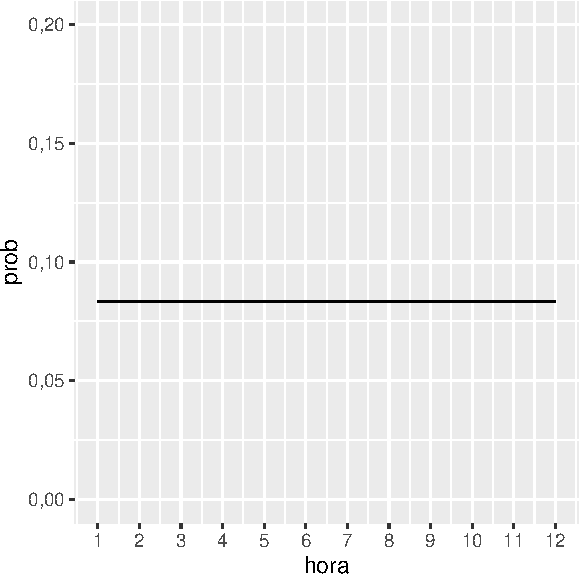
\includegraphics{EstatEcon_files/figure-latex/DistribuicaoUniformeContinua-1.pdf}
\caption{\label{fig:DistribuicaoUniformeContinua}Um exemplo de distribuição uniforme Contínua.}
\end{figure}

Nesta situação apresentada na figura \ref{fig:DistribuicaoUniformeContinua}, matematicamamente faz sentido calcular a probabilidade para um intervalo de valores da variável e não para valores específicos com é no caso da variável aleatória discreta. Dessa forma com a função de probabilidade da distribuição, denominada de \textbf{função densidade de probabilidade} (f.d.p.), pode-se obter a probabilidade obtendo a área abaixo da curva desta função. Matematicamente, a probabilidade pode ser obtida através da integral definida desta função para o intervalo de valores em questão.

Note que para \(f(x)\) ser função densidade de probabilidade, precisa atender as seguintes propriedades definidas pela teoria da probabilidade:

\begin{itemize}
\tightlist
\item
  a soma das probabilidades para todo os valores definidos da variável \(x\) dever ser igual a 1.
\item
  a probabilidade obtida através de \(f(x)\) não pode ser negativa.
\end{itemize}

No exemplo da relógio analógico a probabilidade da hora estar entre 2 e 3 é a área da curva ou reta da distribuição uniforme contínua cujo valor constante da probabilidade é \(1/12\). O intervalo entre 2 e 3 proporciona um intervalo equivalente a unidade, uma vez que intervalo pode ser calculado entre a diferença entre o valor final e o valor inicial. Dessa forma:

\[
P(2 < x < 3) = \dfrac{1}{12} \times \left( 3 - 2 \right) = \dfrac{1}{12},
\]
ou seja,
\[
P(2<x<3) = P(2\leq x \leq 3) = P(2 < x \leq 3) = P(2\leq x < 3) = \dfrac{1}{12}
\]

\textbf{Exemplo numérico sobre função densidade de probabilidade}

Exemplo 4.1.3 da página 79 do \citet{Sartoris2013}. Dada a função densidade de probabilidade da variável aleatória contínua mostrada a seguir

\[
  f(x) = 
    \begin{cases}
      Ax~~0\leq x \leq 3\\
      0,~~X<0~\text{ou}~x>3\\
    \end{cases}
\]

\begin{enumerate}
\def\labelenumi{\alph{enumi})}
\tightlist
\item
  Determine o valor de A.
\end{enumerate}

\textbf{Resposta}: Dado que \(f(x) = Ax\)

\[
  f(3) = 3A
\]
para \(x = 3\) e
\[
  f(0)  = 0
\]
para \(x=0\)

Graficamente seria um triângulo de de base 3 e altura de 3A. Como a função definida de modo que
\[
  f(x) \geq 0
\]
ou seja resulte valores não-negativos, basta igualar a área a 1, pois a soma das probabilidades para todos os valores definidos para a variável \(x\) deve ser igual a 1. Portanto a probabilidade é a área correspondente ao triangulo de base 3 e altura 3A. Ou seja,
\[
  \dfrac{3A \times 3}{2} = 1
\]
e
por isso
\[
  A = \dfrac{2}{9}
\]
Ou seja,
\[
  f(x) = 3x
\]

\begin{enumerate}
\def\labelenumi{\alph{enumi})}
\setcounter{enumi}{1}
\tightlist
\item
  Determine a probabilidade de que \(x\) esteja entre 2 e 3.
\end{enumerate}

Para \(x=2\) se tem
\[
  f(2) = 2\times \dfrac{2}{9} = \dfrac{4}{9}
\]
e para \(x=3\)
\[
f(3) = 3 \times \dfrac{2}{9} = \dfrac{2}{3}
\]
A área correspondente a probababilidade de \(x\) estar entre 2 e 3 pode ser obtida subtraindo a área do triângulo maior que seria com \(x\) entre 0 e 3 e o triângulo menor com \(x\) entre 2 e 3. Ou seja, a área do triangulo maior é calculado como

\[
  \text{triângulo menor} = 3\times \dfrac{2}{3} \times \dfrac{1}{2} = 1
\]

e a área do triângulo menor é calculado como

\[
  \text{triângulo menor} = 2\times \dfrac{4}{9} \times \dfrac{1}{2} = \dfrac{4}{9}.
\]
Assim a diferença das áreas do triângulo maior e do triângulo menor é igual a \(5/9\). Ou seja,

\[
  P(2<x<3) = 1 - \dfrac{4}{9} = \dfrac{5}{9}
\]

\textbf{Segundo exemplo númerico sobre função densidade de probabilidade}

Exemplo 4.1.4 da página 80 do \citet{Sartoris2013}. Dada da f.d.p. ded uma variável aleatória contínua,

\[
  f(x) = 
    \begin{cases}
      Ax^2~~\text{para }~0\leq x \leq 1\\
      0,~~\text{para }~x<0~\text{ou}~x>1\\
    \end{cases}
  \]

\begin{enumerate}
\def\labelenumi{\alph{enumi})}
\tightlist
\item
  Determine o valor da constante A.
  Note que a função já não é mais do tipo linear e por isso não é necessário utilizar a integral da função em questão para calcular a probabilidade. Considerando novamente que a soma das probabilidades para todos os valores definidos para a variável \(x\) deve ser igual a um, se tem
\end{enumerate}

\[
  \int_{-\infty}^{+\infty} f(x)\text{d}x = 1
\]
Para este exemplo, a função \(f(x)\) só está definido para os valores entre 0 e 1, sendo que para valores de \(x\) menor que 0 e valores de \(x\) maior que 1 a função \(f(x)\) assume valor igual a zero. Portanto,

\[
  \int_{0}^{1} Ax^2\text{d}x = 1
\]
Como A é constante, pode-se colocar para fora da integral

\[
  A\int_{0}^{1} x^2\text{d}x = 1
\]
Calculando a integral definida
\[
  A\left[ \dfrac{x^3}{3} \right]_{0}^{1} = 1
\]
Avaliando para os valores 1 e 0 e depois realizando a diferença
\[
  A\left[ \dfrac{1}{3} - \dfrac{0}{3} \right]_{0}^{1} = 1
\]
Ou seja,
\[
  A = 3.
\]
Ou seja a função é

\[
  f(x) = 3x^2.
\]

\begin{enumerate}
\def\labelenumi{\alph{enumi})}
\setcounter{enumi}{1}
\tightlist
\item
  Dtermine a probabilidade de que \(x\) esteja entre 0,5 e 1.
\end{enumerate}

Primeiramente verifica-se que tanto 0,5 como 1 são valores que estão dentro do intervalo de \(x\) definido para a função em questão. Por exemplo, se um dos limites fosse igual a 2, consideraria \(x=1\) pois \(f(x)=0\) para \(x>1\). Por isso basta calcular a integral da função para os valores de \(x\) entre 0,5 e 1. Ou seja,

\[
  P(0,5\leq x \leq 1) = \int_{0,5}^{1} 3x^3\text{d}x 
\]
\[
  P(0,5\leq x \leq 1) = \left[ \frac{3x^3}{3}  \right]_{0,5}^{1}
\]
\[
  P(0,5\leq x \leq 1) = 1^3 - 0,5^3 = 1 - 0,125 = 0,875.
\]
Resumindo, para que uma função qualquer seja uma função densidade de probabilidade precisa atender duas condições:

\[
  \int_{-\infty}^{+\infty} f(x) \text{d}x = 1
\]
e
\[
  f(x) \geq 0~~\text{para todos os valores de}~x
\]

\textbf{Exemplo numérico sobre a distribuição exponencial}

O exemplo 4.1.5 da página 82 de \citet{Sartoris2013} é uma simples aplicação para a distribuição exponencial. Dada a f.d.p. da varíável aleatória contínua \(x\)
\[
  f(x) =
    \begin{cases}
      Ae^{-\alpha x},~~\text{para }~x\geq 0 \\
      0,~~\text{para }~~x<0
    \end{cases}
\]
a) Determine o valor de A.
Então como foi informado no anunciado do exemplo numérico, essa distribuição especial é conhecida com distribuição exponencial. Como

\[
  \int_{-\infty}^{+\infty} f(x) \text{d}x = 1
\]

e a função assume valores iguais a zero para valores negativos de \(x\), se tem

\[
  \int_ {0}^{+\infty} A e^{-\alpha x} = 1.
\]
Como A é constante, pode-se colocar par fora da integral
\[
  A\int_{0}^{+\infty} e^{-\alpha x}\text{d}x = 1
\]
e sabendo que a integral da função é um pouco diferente, considerando que há um \(\alpha\) multiplicando \(x\), temos

\[
  A\left[ \dfrac{e^{-\alpha x}}{-\alpha} \right]_{0}^{+\infty} = 1
\]

\[
  A\left[0  - \left(-\dfrac{1}{\alpha}\right)\right] = 1
\]
Portanto,

\[
A = \alpha
\]

\hypertarget{funuxe7uxe3o-de-distribuiuxe7uxe3o-de-variuxe1veis-contuxednuas}{%
\subsection{Função de distribuição de variáveis contínuas}\label{funuxe7uxe3o-de-distribuiuxe7uxe3o-de-variuxe1veis-contuxednuas}}

A semelhança do caso das variáveis discretas, a \textbf{função de distribuição acumulada } ou \textbf{função de distribuição} \(F(x)\) é a soma da probabilidades de todos os valores possíveis que a variável \(x\) pode assumir até o valor de \(x\) propriamente dito. Isso é feito através da integral da seguinte forma

\[
  F(x) = \int_{-\infty}^{x} f(t) \text{d}t.
\]

Portanto, matematicamente,\(f(x)\) é a derivda da função \(F(x)\)
\[
  f(x) = \dfrac{\text{d}F(x)}{\text{d}x}.
\]

\textbf{Exemplo numérico da função de distribuição}

O exemplo 4.2.1 da página 83 do \citet{Sartoris2013}, trata-se da obtenção da função distribuição exponencial através da sua respectiva função densidade de probabilidade. Dada a função f.d.p.da dsitribuição exponencial, determine a função de distribuição correspondente.

\[
  f(x) = 
  \begin{cases}
    e^{-x},~~\text{para }~ x \geq 0\\
    0,~~\text{para } x< 0
  \end{cases}
\]
Dado que a função só é definido para \(x\geq 0\), o limite de integração inferior é zero.

\[
  F(x) = \int_{0}^{+\infty} f(t)\text{d}t
\]
substituindo a f.d.p.
\[
  F(x) = \int_{0}^{+\infty} e^{-t}\text{d}t
\]
lembrando a integral de \(e^{-x}\) e que todo número elevado a zero é igual a um
\[
  F(x) = \left[ -e^{-t}  \right]_{0}^{x}.
\]
Assim,
\[
  F(x) = -e^{-x} + e^{0}
\]
e
\[
  F(x) = 1 - e^{-x}
\]
Portanto a função distribuição é dada por

\[
  F(x) =
  \begin{cases}
    1 - e^{-x},~~\text{para } x\geq 0 \\
    0,~~\text{para } x\leq 0
  \end{cases}
\]

\textbf{Segundo Exemplo numérico sobre função de distrubuição}

Exemplo 4.2.2 da página 84 de \citet{Sartoris2013}. Seja a função distribuição

\[
  F(x) = 
  \begin{cases}
    0,5(x^3 + 1),~~\text{para } -1\leq x \leq 1\\
    0,~~\text{para }x < -1\\
    1, x > 1
  \end{cases}
\]
determine a função densidade de probabilidade correspondente.

Resposta:

A função densidade de probabilidade é dado por

\[
  f(x) = \dfrac{\text{d}F(x)}{\text{d}x}
\]

\[
  f(x) = \dfrac{\text{d}(0,5 x^2  + 1)}{\text{d}x}
\]

\[
  f(x) = 3 \times 0,5x^2 + 0
\]

\[
  f(x) = 1,5 x^2 
\]

Portanto, a função densidade de probabilidade é:

\[
  f(x) = 
  \begin{cases}
    1,5x^2,~~\text{para } -1\leq x \leq 1\\
    0,~~\text{para }x < -1 ou x > 1
  \end{cases}
\]
A função distribuição \(F(x)\), assim como a função densidade, deve atender dois requisitos:

\begin{itemize}
\tightlist
\item
  não pode ser negativa e deve ser menor ou igual a 1.
\end{itemize}

\[
  0\leq F(x) \leq 1
\],

\begin{itemize}
\tightlist
\item
  a soma das probabilidades de todos os valores da variável é igual a 1.
\end{itemize}

\[
  \lim_{x \rightarrow \infty} F(x) = 1
\].

Estes requisitos são atendidos pelas funções distribuições \(F(x)\) dos exemplos numéricos anteriores.

\hypertarget{esperanuxe7a-e-variuxe2ncia-de-variuxe1veis-aleatuxf3rias-contuxednuas}{%
\subsection{Esperança e variância de variáveis aleatórias contínuas}\label{esperanuxe7a-e-variuxe2ncia-de-variuxe1veis-aleatuxf3rias-contuxednuas}}

A esperança matemática para uma variável aleatória contínua é a soma contínua de todos os valores da variável com sua respectivas probabilidades. Uma soma contínua é a integral e, por sua vez, a probabilidade é encontrada pela função densidade de probabilidade. Dessa forma, matematicamente a esperança é

\[
  E(x) = \int_{-\infty}^{+\infty} x f(x)~\text{d}x. 
\]
A variância por sua vez,

\[
  Var(x) = E[x - E(x)]^2
\]

ou simplesmente

\[
  Var(x) = E[x - \mu]^2
\]
onde \(\mu\) é igual a média de \(x\). Em termos de integral fica

\[
  Var(x) = \int_{-\infty}^{+\infty} (x- \mu)^2 \text{d}x
\]
Alternativamente
\[
  Var(x) = E(x^2) - [E(x)]^2 
\]
que em termos de integral fica
\[
  Var(x) = \int_{-\infty}^{+\infty} x^2 f(x)\text{d}x - \left[\int_{-\infty}^{+\infty} xf(x) \text{d}x \right]^2
\]

\textbf{Exemplo numérico sobre esperança e variância}

Exemplo 4.3.1. da página 85 do \citet{Sartoris2013}. Seja a f.d.p.

\[
  f(x) = 
    \begin{cases}
      3x^2~~\text{para }~0\leq x \leq 1\\
      0,~~\text{para }~x<0~\text{ou}~x>1\\
    \end{cases}
  \]
a) Calcule o valor médio de \(x\).

Resposta:

Como a média pode ser calculada através de \(E(x)\)
\[
  E(x) = \int_{-\infty}^{+\infty} x f(x)~\text{d}x.
\]
se tem
\[
  E(x) = \int_{0}^{1}x3x^2\text{d}x
\]
\[
  E(x) = 3\int_{0}^{1}x^3\text{d}x
\]
Calculando-se a integral
\[
  E(x) = 3\left[ \dfrac{x^4}{4}\right]_{0}^{1}
\]

\[
  E(x) = 3 \times \dfrac{1^4}{4}
\]

\[
  E(x) = \dfrac{3}{4} = 0,75
\]

\begin{enumerate}
\def\labelenumi{\alph{enumi})}
\setcounter{enumi}{1}
\tightlist
\item
  Calcule a variância de \(x\).
\end{enumerate}

Resposta:

Tomando a fórmula da variância alternativa

\[
  Var(x) = E(x^2) - [E(x)]^2 
\]

que em termos de integral é

\[
  Var(x) = \int_{-\infty}^{+\infty} x^2 f(x)\text{d}x -
  \left[\int_{-\infty}^{+\infty} xf(x) \text{d}x \right]^2
\]
verifica-se que só falta só calcular \(E(x^2)\) para poder calcular a variância de \(x\). Ou seja,

\[
  E(x^2) = \int_{0}^{1} X^23x^2 \text{d}x 
\]

\[
  E(x^2) = 3\int_{0}^{1} x^4  \text{d}x 
\]
calculando a integral
\[
  E(x^2) = 3\left[ \dfrac{x^5}{5} \right]_{0}^{1}
\]

\[
  E(x^2) = 3 \times \dfrac{1}{5}
\]

\[
  E(x^2) = \dfrac{3}{5} = 0,6.
\]
Assim a variância é

\[
  Var(x) = E(x^2) - [E(x)]^2
\]

\[
  Var(x) = 0,6 - (0,75)^2 = 0,6 - 0,5625
\]

\[
  Var(x) = 0,0375
\]

\begin{enumerate}
\def\labelenumi{\alph{enumi})}
\setcounter{enumi}{2}
\tightlist
\item
  Calcule o desvio padrão de \(x\).
\end{enumerate}

\[
dp(x) = \sqrt{0,0375}
\]

\[
dp(x) \cong 0,194
\]

\hypertarget{distribuiuxe7uxe3o-normal}{%
\section{Distribuição Normal}\label{distribuiuxe7uxe3o-normal}}

Para entender a distribuição normal, tome a distribuição binomial com uma probabilidade \(p\) igual 0,5 e \(n\) tendendo ao infinito. Graficamente exemplifica-se com \(n=1,2,3,5,10\).

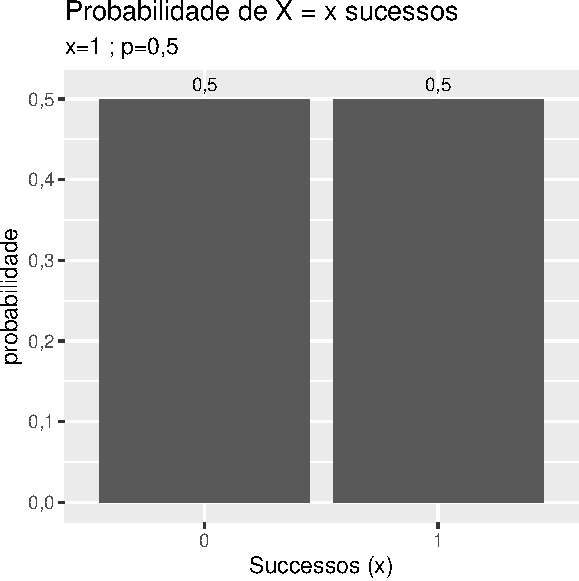
\includegraphics{EstatEcon_files/figure-latex/graficobinomial1-1.pdf}

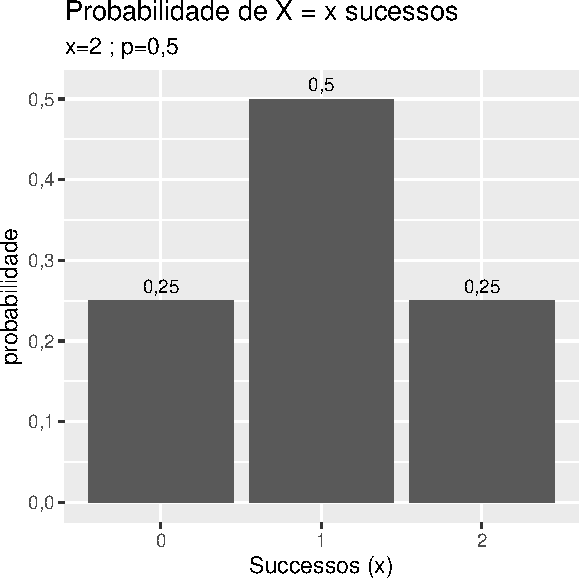
\includegraphics{EstatEcon_files/figure-latex/graficobinomial2-1.pdf}

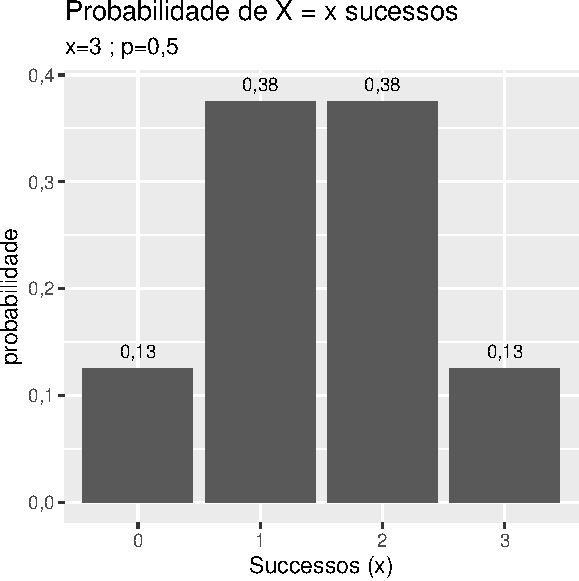
\includegraphics{EstatEcon_files/figure-latex/graficobinomial3-1.pdf}

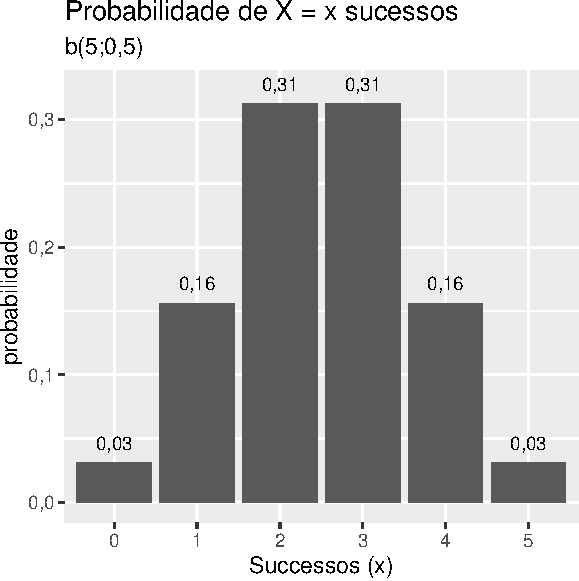
\includegraphics{EstatEcon_files/figure-latex/graficobinomia5-1.pdf}

\begin{figure}
\centering
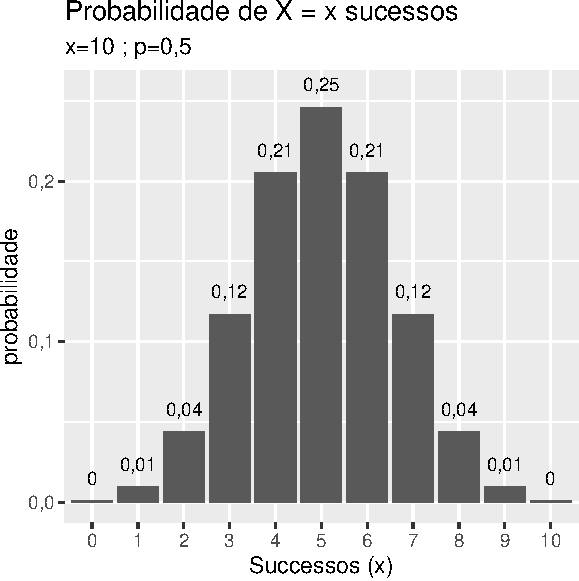
\includegraphics{EstatEcon_files/figure-latex/graficobinomial10-1.pdf}
\caption{\label{fig:graficobinomial10}Da distribuição Binamial para a Distribuição Normal}
\end{figure}

Note na figura \ref{fig:graficobinomial10} que a medida que \(n\) aumenta a distribuição binomial assume um formato que é a de uma típica distribuição normal. Se no limite \(n\) tende ao infinito, a distribuição binomial perde o aspecto discreto na foma de ``escada'' e passa a ter um formato e aspecto de distribuição normal, figura \ref{fig:DistribuicaoNormal0}, que é a referência para uma distribuição de variável aleatória contínua.

\begin{figure}
\centering
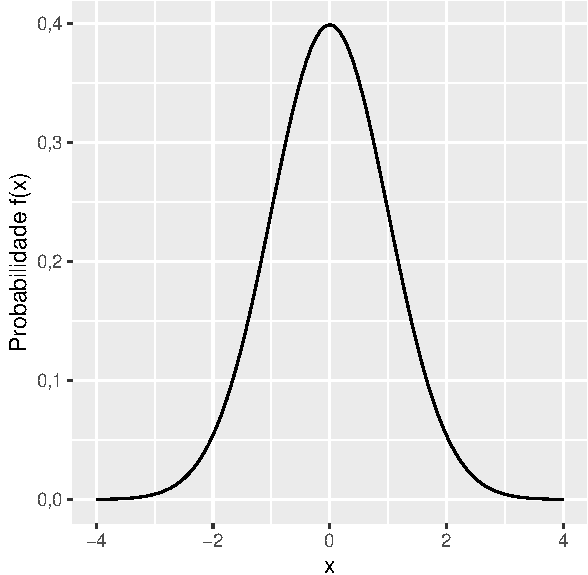
\includegraphics{EstatEcon_files/figure-latex/DistribuicaoNormal0-1.pdf}
\caption{\label{fig:DistribuicaoNormal0}A distribuição Normal}
\end{figure}

Essa distribuição de probabilidade é conhecida com \textbf{normal} ou \textbf{gaussiana} e a sua função densidade de probabilidade é dada por:

\[
  f(x) = \dfrac{1}{\sqrt{2\pi\sigma^2}}e^{\frac{(x-\mu)^2}{2\sigma^2}}
  \label{eq:fdpNormal}
\]

onde \(\mu\) é a média e \(\sigma\) é o desvio padrão da variável \(x\). Se a variável \(x\) tem distribuição normal ou é normalmente distribuída, é usual escrever com notação matemática da seguinte forma

\[
  x \sim N(\mu,\sigma)
\]

e deve ser lida da seguinte forma: \emph{\(x\) segue uma distribuição normal com média \(\mu\) e desvio padrão \(\sigma\)}. Em vez de desvio padrão essa notação matemática pode ter a variância \(\sigma^2\) no lugar do desvio padrão \(\sigma\).

Na função densidade de probabilidade da distribuição normal \eqref{eq:fdpNormal} os parâmetros média \(\mu\) e desvio padrão \(\sigma\) definem uma família de distribuições normais para a variável \(x\).

O parâmetro média \(\mu\) determina a posição da curva em relação à origem, enquanto o desvio padrão \(\sigma\) determina se a curva será mais \textbf{``gorda''}, ou seja, mais dispersa com maior desvio padrão, ou mais \textbf{``magra''}, ou seja mais concentrada com um desvio padrão menor.

O cálculo das probabilidades sob uma distribuição normal é bastante trabalhosa, uma vez que não existe uma função cuja derivada é \(e^{-x^2}\) e, por isso, o cálculo é feito por métodos numéricos. Por isso, tabela-se os valores das integrais da distribuição normal padronizada, ou seja, a distribuição normal com média \(\mu\) igual a zero e desvio padrão \(\sigma\) igual a zero.

\[
  \mu = 0
\]

e

\[
  \sigma = 1
\]

As variáveis normalmente distribuídas com média \(\mu\) diferente de zero e desvio padrão \(\sigma\) diferente de um

\[
  \mu \neq 0
\]

e

\[
  \sigma \neq 1
\]

podem ter os valores das probabilidades obtidas das tabelas de valores para uma distribuição normal padronizada, padronizando a variável \(x\), por exemplo, da seguinte forma

\[
  z = \dfrac{x - \mu}{\sigma}
\]

onde a variável \(z\) tem distribuição normal com média \(\mu\) igual a zero e desvio padrão \(\sigma\) igual a 1. Ou seja possui um distribuição normal padronizada para a qual pode-se usar os valores calculados e disponibilizados em tabelas que se encontram no apêndice da maioria dos livros de estatística e econometria. Na tabela com os valores da distribuição normal padronizada, usualmente denota-se a variável normal padronizada como \(z\). Outro detalhe da tabela da dstribuição normal padronizada é a disponibilidade dos valores das probabilidades para a metade da distribuição, ou seja, para os valores positivos de \(z\) pelo fato da distribuição normal ser simétrica. Portanto,
\[
  P(0 < z < 1,23) = P(-1,23 < z < 0).
\]
Dessa forma, o maior valor de probabilidade encontrada na tabela para uma distribuição normal padronizada usualmente é aproximadamente igual a 0,5. Claro, existem tabelas que podem apresentar os valores para toda a distribuição e nestes casos o maior valor será aproximadamente igual a 1, pois os valores são em termos de função distribuição de probabilidade \(F(z)\).
Usando o R, a probabilidade de \(z\) estar entre zero e 1,23 é calculada através da função \texttt{pnorm} que entrega o valor de \(F(z)\).

\begin{Shaded}
\begin{Highlighting}[]
\NormalTok{p0z1}\FloatTok{.23}\NormalTok{ <-}\StringTok{ }\KeywordTok{round}\NormalTok{(}\KeywordTok{pnorm}\NormalTok{(}\FloatTok{1.23}\NormalTok{, }\DataTypeTok{mean =} \DecValTok{0}\NormalTok{, }\DataTypeTok{sd =} \DecValTok{1}\NormalTok{) }\OperatorTok{-}\StringTok{ }\KeywordTok{pnorm}\NormalTok{(}\DecValTok{0}\NormalTok{, }
    \DataTypeTok{mean =} \DecValTok{0}\NormalTok{, }\DataTypeTok{sd =} \DecValTok{1}\NormalTok{), }\DecValTok{4}\NormalTok{)}
\NormalTok{p0z1}\FloatTok{.23}
\end{Highlighting}
\end{Shaded}

\begin{verbatim}
## [1] 0,3907
\end{verbatim}

Ou seja

\[
  P(0 < z < 1,23) = F(1,23) - F(0) \cong \text{0,3907}.
\]

Graficamente, usando o pacote \texttt{ggplot2}, fica mais fácil de visulizar a probabilidade de \(z\) estar entre zero e 1,23 que de é de \text{0,3907} na figura \ref{fig:ExemploDistribuicaoNormalPadronizada1} que corresponde à área colorida.

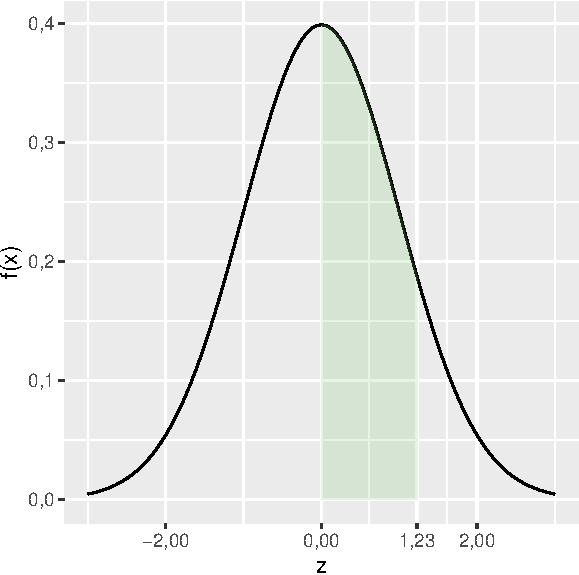
\includegraphics{EstatEcon_files/figure-latex/ExemploDistribuicaoNormalPadronizada1-1.pdf}
Note que o valor \text{0,3907} é o valor encontrado diretamente na tabela que apresenta valores de probabilidade somente para metade da distribuição, neste caso para \(0<z<+\infty\).

Quando os valores de \(z\) são maiores que zero, se tem uma outra situação que comumente aparece nos exercícios. Seja a probabilidade de \(z\) estar entre 0,27 e 1,43. Ou seja,

\[
  P(0,27 < z < 1,43) 
\]

Note que a probabiliade corresponde à área que está abaixo da curva da função densidade de probabilidade para \(z\) entre 0,27 e 1,43. Ou seja, a integral de \(f(z)\) entre 0,27 e 1,43. Usando-se a função distribuição de probabilidade \(F(z)\) corresponde a diferença entre \(F(1,43)\) e \(F(,27)\)

\[
  P(0,27 < z < 1,43) = F(1,43) - F(0,27)
\]

Na figura \ref{fig:ExemploDistribuicaoNormalPadronizada2} fica claro o por quê da diferença entre \(F(z)\). Note que aqui a ideia é válida tanto para a metade da distribuição como para a distribuição completa incluindo a parte em que \(z<0\).

\begin{figure}
\centering
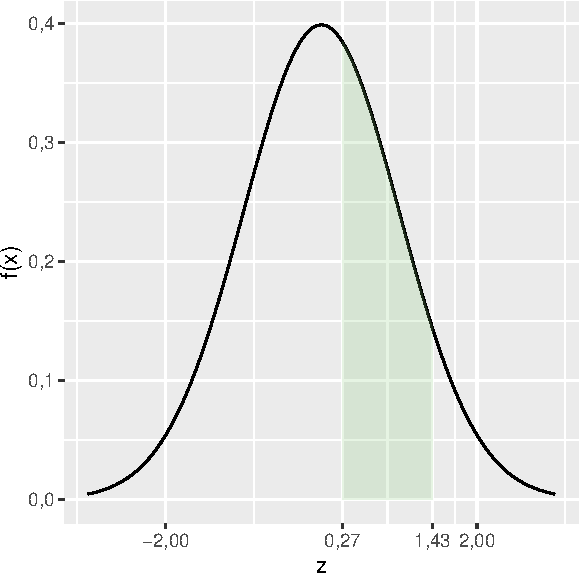
\includegraphics{EstatEcon_files/figure-latex/ExemploDistribuicaoNormalPadronizada2-1.pdf}
\caption{\label{fig:ExemploDistribuicaoNormalPadronizada2}Probabilidade z entre 0,27 e 1,43}
\end{figure}

Para a situação em que se tem os valores das probabilidades tabulados somente para metade da distribuição se tem

\[
  P(0,27 < z < 1,43) = P(0 < z < 1,43) - P(0 < z < 0,27),
\]
ou seja,
\[
  P(0,27 < z < 1,43) = [F(1,43) - F(0)] - [F(0,27) - F(0)].
\]

Usando o R, a probabilidade de \(z\) estar entre 0,27 e 1,43 pode ser calculada da seguinte forma

\begin{Shaded}
\begin{Highlighting}[]
\CommentTok{# Calculo de F(1,43) - F(0)}

\NormalTok{p2 <-}\StringTok{ }\KeywordTok{round}\NormalTok{(}\KeywordTok{pnorm}\NormalTok{(}\FloatTok{1.43}\NormalTok{, }\DataTypeTok{mean =} \DecValTok{0}\NormalTok{, }\DataTypeTok{sd =} \DecValTok{1}\NormalTok{, }\DataTypeTok{lower.tail =}\NormalTok{ T) }\OperatorTok{-}\StringTok{ }
\StringTok{    }\KeywordTok{pnorm}\NormalTok{(}\DecValTok{0}\NormalTok{, }\DataTypeTok{mean =} \DecValTok{0}\NormalTok{, }\DataTypeTok{sd =} \DecValTok{1}\NormalTok{, }\DataTypeTok{lower.tail =}\NormalTok{ T), }\DecValTok{4}\NormalTok{)}

\NormalTok{p2}
\end{Highlighting}
\end{Shaded}

\begin{verbatim}
## [1] 0,4236
\end{verbatim}

\begin{Shaded}
\begin{Highlighting}[]
\CommentTok{# Calculo de F(0,27) - F(0)}

\NormalTok{p1 <-}\StringTok{ }\KeywordTok{round}\NormalTok{(}\KeywordTok{pnorm}\NormalTok{(}\FloatTok{0.27}\NormalTok{, }\DataTypeTok{mean =} \DecValTok{0}\NormalTok{, }\DataTypeTok{sd =} \DecValTok{1}\NormalTok{, }\DataTypeTok{lower.tail =}\NormalTok{ T) }\OperatorTok{-}\StringTok{ }
\StringTok{    }\KeywordTok{pnorm}\NormalTok{(}\DecValTok{0}\NormalTok{, }\DataTypeTok{mean =} \DecValTok{0}\NormalTok{, }\DataTypeTok{sd =} \DecValTok{1}\NormalTok{, }\DataTypeTok{lower.tail =}\NormalTok{ T), }\DecValTok{4}\NormalTok{)}

\NormalTok{p1}
\end{Highlighting}
\end{Shaded}

\begin{verbatim}
## [1] 0,1064
\end{verbatim}

\begin{Shaded}
\begin{Highlighting}[]
\CommentTok{# Calculo de P(0,27 < z < 1,43)}

\NormalTok{p027z143 <-}\StringTok{ }\NormalTok{p2 }\OperatorTok{-}\StringTok{ }\NormalTok{p1}

\NormalTok{p027z143}
\end{Highlighting}
\end{Shaded}

\begin{verbatim}
## [1] 0,3172
\end{verbatim}

Portanto,

\[
  P(0,27 < z < 1,43) = \text{0,4236} - \text{0,1064} = \text{0,3172}.
\]

Alternativamente, se tem os valores das probabilidades para a distribuição completa na tabela ou se está usando o R para os cálculos

\[
  P(0,27 < z < 1,43) = F(1,43) - F(0,27)
\]

Usando o R, o cálculo da probabilidade de \(z\) estar entre 0,27 e 1,43 é simplesmente

\begin{Shaded}
\begin{Highlighting}[]
\NormalTok{p027z143r <-}\StringTok{ }\KeywordTok{round}\NormalTok{(}\KeywordTok{pnorm}\NormalTok{(}\FloatTok{1.43}\NormalTok{, }\DataTypeTok{mean =} \DecValTok{0}\NormalTok{, }\DataTypeTok{sd =} \DecValTok{1}\NormalTok{, }\DataTypeTok{lower.tail =} \OtherTok{TRUE}\NormalTok{) }\OperatorTok{-}\StringTok{ }
\StringTok{    }\KeywordTok{pnorm}\NormalTok{(}\FloatTok{0.27}\NormalTok{, }\DataTypeTok{mean =} \DecValTok{0}\NormalTok{, }\DataTypeTok{sd =} \DecValTok{1}\NormalTok{, }\DataTypeTok{lower.tail =} \OtherTok{TRUE}\NormalTok{), }
    \DecValTok{4}\NormalTok{)}

\CommentTok{# Calculo de F(1,43)}

\NormalTok{p2r <-}\StringTok{ }\KeywordTok{round}\NormalTok{(}\KeywordTok{pnorm}\NormalTok{(}\FloatTok{1.43}\NormalTok{, }\DataTypeTok{mean =} \DecValTok{0}\NormalTok{, }\DataTypeTok{sd =} \DecValTok{1}\NormalTok{, }\DataTypeTok{lower.tail =}\NormalTok{ T), }
    \DecValTok{4}\NormalTok{)}

\NormalTok{p2r}
\end{Highlighting}
\end{Shaded}

\begin{verbatim}
## [1] 0,9236
\end{verbatim}

\begin{Shaded}
\begin{Highlighting}[]
\CommentTok{# Calculo de F(0,27)}

\NormalTok{p1r <-}\StringTok{ }\KeywordTok{round}\NormalTok{(}\KeywordTok{pnorm}\NormalTok{(}\FloatTok{0.27}\NormalTok{, }\DataTypeTok{mean =} \DecValTok{0}\NormalTok{, }\DataTypeTok{sd =} \DecValTok{1}\NormalTok{, }\DataTypeTok{lower.tail =}\NormalTok{ T), }
    \DecValTok{4}\NormalTok{)}

\NormalTok{p1r}
\end{Highlighting}
\end{Shaded}

\begin{verbatim}
## [1] 0,6064
\end{verbatim}

\begin{Shaded}
\begin{Highlighting}[]
\CommentTok{# Calculo de P(0,27 < z < 1,43)}

\NormalTok{p027z143r <-}\StringTok{ }\NormalTok{p2r }\OperatorTok{-}\StringTok{ }\NormalTok{p1r}


\NormalTok{p027z143r}
\end{Highlighting}
\end{Shaded}

\begin{verbatim}
## [1] 0,3172
\end{verbatim}

Portanto,

\[
  P(0,27 < z < 1,43) = \text{0,9236} - \text{0,6064} = \text{0,3172}.
\]

Uma outra situação bastante comum nos exercícios é quando o limite inferior do intervalo é negativo e valor do limite superior é positivo. Considere o cálculo da probabilidade de \(z\) estar entre -1,38 e 0,97. Na figura \ref{fig:ExemploDistribuicaoNormalPadronizada3} fica mais fácil visualizar qual a área a ser calculada que corresponde a probabilidade solicitada.

\begin{figure}
\centering
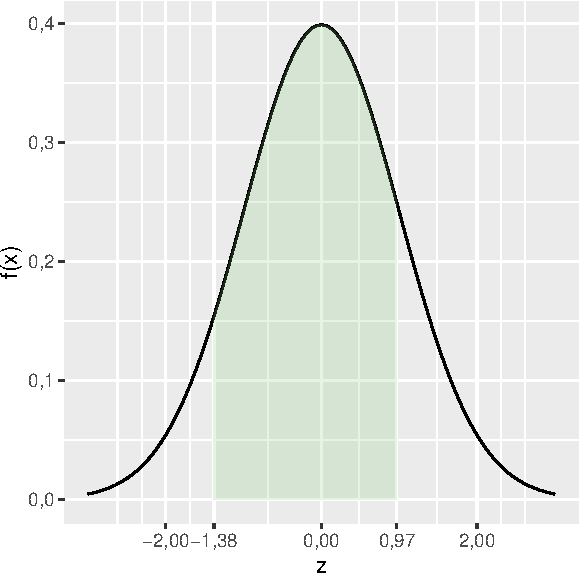
\includegraphics{EstatEcon_files/figure-latex/ExemploDistribuicaoNormalPadronizada3-1.pdf}
\caption{\label{fig:ExemploDistribuicaoNormalPadronizada3}Probabilidade z entre -1,38 e 0,97}
\end{figure}

Considerando a situação em que a tabela tem apenas metade dos valores de probabilidade para a distribuição normal padronizada, o cálculo é

\[
  P( -1,38 < z < 0,97) = P (-1,38 < z < 0) + P(0 < z < 0,97).
\]
Como a distribuição normal é simétrica, pode-se escrever
\[
  P( -1,38 < z < 0,97) = P (0 < z < 1,38) + P(0 < z < 0,97)
\]
ou
\[
  P( -1,38 < z < 0,97) = [F(1,38) - F(0)] +[F(0,97) - F(0)]
\]

Usando o R, a probabilidade de \(z\) estar entre 0,27 e 1,43 pode ser calculada da seguinte forma

\begin{Shaded}
\begin{Highlighting}[]
\CommentTok{# Calculo de F(1,38) - F(0)}

\NormalTok{pf138f0 <-}\StringTok{ }\KeywordTok{round}\NormalTok{(}\KeywordTok{pnorm}\NormalTok{(}\FloatTok{1.38}\NormalTok{, }\DataTypeTok{mean =} \DecValTok{0}\NormalTok{, }\DataTypeTok{sd =} \DecValTok{1}\NormalTok{, }\DataTypeTok{lower.tail =}\NormalTok{ T) }\OperatorTok{-}\StringTok{ }
\StringTok{    }\KeywordTok{pnorm}\NormalTok{(}\DecValTok{0}\NormalTok{, }\DataTypeTok{mean =} \DecValTok{0}\NormalTok{, }\DataTypeTok{sd =} \DecValTok{1}\NormalTok{, }\DataTypeTok{lower.tail =}\NormalTok{ T), }\DecValTok{4}\NormalTok{)}

\NormalTok{pf138f0}
\end{Highlighting}
\end{Shaded}

\begin{verbatim}
## [1] 0,4162
\end{verbatim}

\begin{Shaded}
\begin{Highlighting}[]
\CommentTok{# Calculo de F(0,97) - F(0)}

\NormalTok{pf097f0 <-}\StringTok{ }\KeywordTok{round}\NormalTok{(}\KeywordTok{pnorm}\NormalTok{(}\FloatTok{0.97}\NormalTok{, }\DataTypeTok{mean =} \DecValTok{0}\NormalTok{, }\DataTypeTok{sd =} \DecValTok{1}\NormalTok{, }\DataTypeTok{lower.tail =}\NormalTok{ T) }\OperatorTok{-}\StringTok{ }
\StringTok{    }\KeywordTok{pnorm}\NormalTok{(}\DecValTok{0}\NormalTok{, }\DataTypeTok{mean =} \DecValTok{0}\NormalTok{, }\DataTypeTok{sd =} \DecValTok{1}\NormalTok{, }\DataTypeTok{lower.tail =}\NormalTok{ T), }\DecValTok{4}\NormalTok{)}

\NormalTok{pf097f0}
\end{Highlighting}
\end{Shaded}

\begin{verbatim}
## [1] 0,334
\end{verbatim}

\begin{Shaded}
\begin{Highlighting}[]
\CommentTok{# Calculo de P(1,38 < z < 0,97)}

\NormalTok{p138z097 <-}\StringTok{ }\NormalTok{pf138f0 }\OperatorTok{+}\StringTok{ }\NormalTok{pf097f0}

\NormalTok{p138z097}
\end{Highlighting}
\end{Shaded}

\begin{verbatim}
## [1] 0,7502
\end{verbatim}

Portanto,

\[
  P(0,27 < z < 1,43) = \text{0,4162} - \text{0,334} = \text{0,7502}.
\]

Alternativamente, se tem os valores das probabilidades para a distribuição completa na tabela ou se está usando o R para os cálculos, calcula-se

\[
  P(-0,38 < z < 0,97) = F(0,97) - F(-1,38).
\]

Por que o valor de \(F(0,97)\) é maior que \(F(-1,38)\) e nesta situação se calcula a diferença e não a soma?

Usando o R, o cálculo da probabilidade de \(z\) estar entre -1,38 e 0,97 é simplesmente

\begin{Shaded}
\begin{Highlighting}[]
\NormalTok{p138z097r <-}\StringTok{ }\KeywordTok{round}\NormalTok{(}\KeywordTok{pnorm}\NormalTok{(}\OperatorTok{-}\FloatTok{1.38}\NormalTok{, }\DataTypeTok{mean =} \DecValTok{0}\NormalTok{, }\DataTypeTok{sd =} \DecValTok{1}\NormalTok{, }\DataTypeTok{lower.tail =} \OtherTok{TRUE}\NormalTok{) }\OperatorTok{-}\StringTok{ }
\StringTok{    }\KeywordTok{pnorm}\NormalTok{(}\FloatTok{0.97}\NormalTok{, }\DataTypeTok{mean =} \DecValTok{0}\NormalTok{, }\DataTypeTok{sd =} \DecValTok{1}\NormalTok{, }\DataTypeTok{lower.tail =} \OtherTok{TRUE}\NormalTok{), }
    \DecValTok{4}\NormalTok{)}

\CommentTok{# Calculo de F(-1,38)}

\NormalTok{pf138r <-}\StringTok{ }\KeywordTok{round}\NormalTok{(}\KeywordTok{pnorm}\NormalTok{(}\OperatorTok{-}\FloatTok{1.38}\NormalTok{, }\DataTypeTok{mean =} \DecValTok{0}\NormalTok{, }\DataTypeTok{sd =} \DecValTok{1}\NormalTok{, }\DataTypeTok{lower.tail =}\NormalTok{ T), }
    \DecValTok{4}\NormalTok{)}

\NormalTok{pf138r}
\end{Highlighting}
\end{Shaded}

\begin{verbatim}
## [1] 0,0838
\end{verbatim}

\begin{Shaded}
\begin{Highlighting}[]
\CommentTok{# Calculo de F(0,97)}

\NormalTok{pf097r <-}\StringTok{ }\KeywordTok{round}\NormalTok{(}\KeywordTok{pnorm}\NormalTok{(}\FloatTok{0.97}\NormalTok{, }\DataTypeTok{mean =} \DecValTok{0}\NormalTok{, }\DataTypeTok{sd =} \DecValTok{1}\NormalTok{, }\DataTypeTok{lower.tail =}\NormalTok{ T), }
    \DecValTok{4}\NormalTok{)}

\NormalTok{pf097r}
\end{Highlighting}
\end{Shaded}

\begin{verbatim}
## [1] 0,834
\end{verbatim}

\begin{Shaded}
\begin{Highlighting}[]
\CommentTok{# Calculo de P(-1,38 < z < 0,97)}

\NormalTok{p138z097r <-}\StringTok{ }\NormalTok{pf097r }\OperatorTok{-}\StringTok{ }\NormalTok{pf138r}


\NormalTok{p138z097r}
\end{Highlighting}
\end{Shaded}

\begin{verbatim}
## [1] 0,7502
\end{verbatim}

Portanto,

\[
  P(0,27 < z < 1,43) = \text{0,834} - \text{0,0838} = \text{0,7502}.
\]

Uma outra situação bastante interessante e comum nos exercícios sobre a aplicação de distribuição normal padronizada é quando se pede o cálculo da probabilidade de \(z\) ser maior que um determinado valor. Nestas situações, a palavra chave é \textbf{pelo menos}. Considere a situação na qual se pede o cálculo da probabilidade de que \(z\) seja maior que 2,22. Ou seja,

\[
P(z > 2,22)
\]

Na figura \ref{fig:ExemploDistribuicaoNormalPadronizada4} fica claro onde fica a área correspondente a probabilidade solicitada.

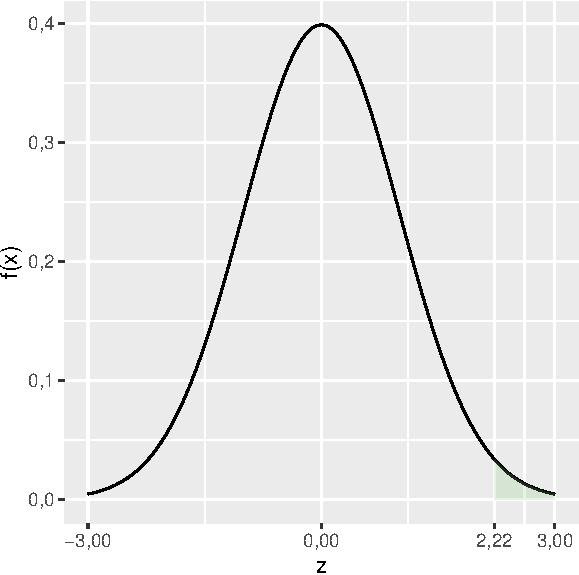
\includegraphics{EstatEcon_files/figure-latex/ExemploDistribuicaoNormalPadronizada4-1.pdf}
Dessa forma, o cálculo considerando a disponibilidade da metade dos valores da distribuição normal padronizada é

\[
  P(z>2,22) = 0,5 - P(0 < z < 2,22) = 0,5 - [F(2,22) - F(0)]
\]
Usando o R, o cálculo é

\begin{Shaded}
\begin{Highlighting}[]
\NormalTok{f222 <-}\StringTok{ }\KeywordTok{round}\NormalTok{(}\KeywordTok{pnorm}\NormalTok{(}\FloatTok{2.22}\NormalTok{, }\DataTypeTok{mean =} \DecValTok{0}\NormalTok{, }\DataTypeTok{sd =} \DecValTok{1}\NormalTok{, }\DataTypeTok{lower.tail =}\NormalTok{ T), }
    \DecValTok{4}\NormalTok{)}
\NormalTok{f222}
\end{Highlighting}
\end{Shaded}

\begin{verbatim}
## [1] 0,9868
\end{verbatim}

\begin{Shaded}
\begin{Highlighting}[]
\NormalTok{f0 <-}\StringTok{ }\KeywordTok{round}\NormalTok{(}\KeywordTok{pnorm}\NormalTok{(}\DecValTok{0}\NormalTok{, }\DataTypeTok{mean =} \DecValTok{0}\NormalTok{, }\DataTypeTok{sd =} \DecValTok{1}\NormalTok{, }\DataTypeTok{lower.tail =}\NormalTok{ T), }
    \DecValTok{4}\NormalTok{)}
\NormalTok{f0}
\end{Highlighting}
\end{Shaded}

\begin{verbatim}
## [1] 0,5
\end{verbatim}

\begin{Shaded}
\begin{Highlighting}[]
\NormalTok{pf222f0 <-}\StringTok{ }\NormalTok{f222 }\OperatorTok{-}\StringTok{ }\NormalTok{f0}

\NormalTok{pf222f0}
\end{Highlighting}
\end{Shaded}

\begin{verbatim}
## [1] 0,4868
\end{verbatim}

\begin{Shaded}
\begin{Highlighting}[]
\NormalTok{pz222 <-}\StringTok{ }\FloatTok{0.5} \OperatorTok{-}\StringTok{ }\NormalTok{pf222f0}

\NormalTok{pz222}
\end{Highlighting}
\end{Shaded}

\begin{verbatim}
## [1] 0,0132
\end{verbatim}

Portanto,

\[
  P(z>2,22) = 0,5 - P(0 < z < 2,22) = 0,5 - \text{0,4868} = \text{0,0132}. 
\]

Alternativamente se tem os valores da probabilidade para a distribuição completa ou se está usando o R para os cálculos

\[
  P(z >2,22) = 1 - F(2,22)
\]

Usando o R para o cálculo,

\begin{Shaded}
\begin{Highlighting}[]
\NormalTok{pz222r <-}\StringTok{ }\DecValTok{1} \OperatorTok{-}\StringTok{ }\KeywordTok{round}\NormalTok{(}\KeywordTok{pnorm}\NormalTok{(}\FloatTok{2.22}\NormalTok{, }\DataTypeTok{mean =} \DecValTok{0}\NormalTok{, }\DataTypeTok{sd =} \DecValTok{1}\NormalTok{, }\DataTypeTok{lower.tail =}\NormalTok{ T), }
    \DecValTok{4}\NormalTok{)}

\NormalTok{pz222r}
\end{Highlighting}
\end{Shaded}

\begin{verbatim}
## [1] 0,0132
\end{verbatim}

Como nem todas as variáveis com distribuição normal tem \(\mu=0\) e \(\sigma = 1\), deve-se padronizá-las para usar os valores da tabela com a distribuição normal padronizada. Seja a variável \(x\) com distribuição normal com \(\mu\neq0\) e \(\sigma \neq 1\). A transformação de \(x\) para que se torne padronizada é

\[
  z = \dfrac{x - \mu}{\sigma}
  \label{eq:PadronizacaoNormal}
\]
onde \(z\), com \(\mu = 0\) e \(\sigma = 1\), é a variável \(x\) transformada.

\textbf{Prova}:

Como \(\sigma\) e \(\mu\) são constantes

\[
  E(z) = \sum_{i=1}^{n} \left(\dfrac{x - \mu}{\sigma}\right) =
  \dfrac{1}{\sigma}\sum_{i=1}^{n}(x - \mu) = \dfrac{1}{\sigma}\times 0 = 0
\]

Pois a soma do desvios em relação à media \(\mu\) é sempre zero.

Aplicando a definição de variância em \(z\) sabendo-se que \(E(z)=0\) e \(E[x-\mu]^2 = \sigma^2\) ou \(dp(x) = \sigma\)

\[
  Var(z) = E[z - E(z)]^2 = E\left[\dfrac{x-\mu}{\sigma}\right]^2 =
  \dfrac{1}{\sigma^2} E[x - \mu]^2 = \dfrac{1}{\sigma^2}\times \sigma^2 = 1.
\]

Assim , através de \eqref{eq:PadronizacaoNormal}, pode-se padronizar qualquer variável que segue uma distribuição normal e que tenha \(\mu\neq 0\) e \(\sigma \neq 1\).

\textbf{Exemplo numérico sobre a padronização}

Exemplo 4.4.1 da página 93 do \citet{Sartoris2013}. O faturamento mensal de uma loja segue uma distribuição normal com média R\$20.000,00 e desvio padrão R\$4.000,00. Calcule a probabilidade de que, em determinado mês, o faturamento eseteja entre R\$19.000,00 e R\$25.000,00.

\textbf{Resposta}:

A variável em questão, faturamento mensal, é normal mas não é padronizada. Por isso, é necessário padronizar os valores antes de utilizar a tabela, cujos valores são para uma distribuição normal padronizada com \(\mu=0\) e \(\sigma =1\).
Para 19.000

\[
  z_1 = \dfrac{x_1 -\mu}{\sigma} = \dfrac{19.000 - 20.000}{4.000} = -0,25
\]
e para 25.000
\[
  z_2 = \dfrac{x_2 - \mu}{\sigma} = \dfrac{25.000-20.000}{4.000} = 1,25.
\]
Portanto
\[
  P(19.000 < x <25.000) = P(-0,25 < z < 1,25)
\]
Como a distribuição normal é simétrica
\[
  P(19.000 < x <25.000) = P(-0,25 < z < 0) + P(0 < z < 1,25)
\]
\[
  P(19.000 < x <25.000) = P(0,< z < 0,25) + P(0 < z < 1,25)
\]
Se a tabela apresenta valores para a distribuição completa
\[
  P(19.000 < x <25.000) = [F(0,25) - F(0)]  + [F(1,25) - F(0)]
\]
ou se a tabela só apresenta valores para a metade da dstribuição
\[
  P(19.000 < x <25.000) = F(0,25)  + F(1,25)].
\]
Mas para qualquer um dos dois caminhos

\[
  P(19.000 < x <25.000) = F(0,25)  +  F(1,25)
\]

Usando o R para os cálculos intermediários, se tem

\begin{Shaded}
\begin{Highlighting}[]
\CommentTok{# Calculo de F(1,25) - F(0)}

\NormalTok{pf125f0 <-}\StringTok{ }\KeywordTok{round}\NormalTok{(}\KeywordTok{pnorm}\NormalTok{(}\FloatTok{1.25}\NormalTok{, }\DataTypeTok{mean =} \DecValTok{0}\NormalTok{, }\DataTypeTok{sd =} \DecValTok{1}\NormalTok{, }\DataTypeTok{lower.tail =}\NormalTok{ T) }\OperatorTok{-}\StringTok{ }
\StringTok{    }\KeywordTok{pnorm}\NormalTok{(}\DecValTok{0}\NormalTok{, }\DataTypeTok{mean =} \DecValTok{0}\NormalTok{, }\DataTypeTok{sd =} \DecValTok{1}\NormalTok{, }\DataTypeTok{lower.tail =}\NormalTok{ T), }\DecValTok{4}\NormalTok{)}

\NormalTok{pf125f0}
\end{Highlighting}
\end{Shaded}

\begin{verbatim}
## [1] 0,3944
\end{verbatim}

\begin{Shaded}
\begin{Highlighting}[]
\CommentTok{# Calculo de F(0,25) - F(0)}

\NormalTok{pf025f0 <-}\StringTok{ }\KeywordTok{round}\NormalTok{(}\KeywordTok{pnorm}\NormalTok{(}\FloatTok{0.25}\NormalTok{, }\DataTypeTok{mean =} \DecValTok{0}\NormalTok{, }\DataTypeTok{sd =} \DecValTok{1}\NormalTok{, }\DataTypeTok{lower.tail =}\NormalTok{ T) }\OperatorTok{-}\StringTok{ }
\StringTok{    }\KeywordTok{pnorm}\NormalTok{(}\DecValTok{0}\NormalTok{, }\DataTypeTok{mean =} \DecValTok{0}\NormalTok{, }\DataTypeTok{sd =} \DecValTok{1}\NormalTok{, }\DataTypeTok{lower.tail =}\NormalTok{ T), }\DecValTok{4}\NormalTok{)}

\NormalTok{pf025f0}
\end{Highlighting}
\end{Shaded}

\begin{verbatim}
## [1] 0,0987
\end{verbatim}

\begin{Shaded}
\begin{Highlighting}[]
\CommentTok{# Calculo de P(-0,25 < z < 1,25)}

\NormalTok{p025z125 <-}\StringTok{ }\NormalTok{pf025f0 }\OperatorTok{+}\StringTok{ }\NormalTok{pf125f0}

\NormalTok{p025z125}
\end{Highlighting}
\end{Shaded}

\begin{verbatim}
## [1] 0,4931
\end{verbatim}

Ou seja,

\[
  P(19.000 < x <25.000) = F(0,25)  +  F(1,25) = \text{0,0987} + \text{0,3944}
\]

\[
  P(19.000 < x <25.000) = \text{0,4931}.
\]

\hypertarget{teorema-de-tchebichev}{%
\section{Teorema de Tchebichev}\label{teorema-de-tchebichev}}

Se a função densidade de uma variável aleatória é conhecida, pode-se conhecer sua média e variância. Por outro lado, se são conhecidas somente a média e a variância de uma variável aleatória, não é possível conhecer a sua respectiva função densidade de probabilidade. Mas é possível definir um limite para uma distribuição de probabilidade qualquer, seja discreta ou acontínua, que é dado pelo teorema de Tchebichev.

\textbf{Teorema de Tchebichev}

seja uma variável aleatória \(x\) com média \(\mu\) e desvio padrão \(\sigma\). A probabilidade de que a variável \(x\) esteja acima ou abaixo da média que não supere, em módulo, \(k\) desvio padrão, é maior ou pelo menos igual a \(1 - 1/k^2\). Ou seja,

\[
  P(|x - \mu| <k\sigma) \geq 1-\dfrac{1}{k^2}.
\]
Consequentemente, a probabilidade de que a variável \(x\) esteja acima ou abaixo da média supere ou seja igual, em módulo, a \(k\) desvio padrão é menor ou pelo menos igual a \(1/k^2\). Ou seja,
\[
  P(|x-\mu| \geq k\sigma) \leq \dfrac{1}{k^2}
\]
Essas duas relações dão um limite universal ao desvio \(|x-\mu|\) em termos de \(\sigma\).

Assumindo, por exemplo, que \(k = 2\), se tem

\[
  P(|x - \mu| <2\sigma) \geq 1-\dfrac{1}{2^2}
\]

\[
  P(|x - \mu| <2\sigma) \geq 0,75 = 75\%
\]
ou
\[
  P(|x-\mu| \geq 2\sigma) \leq \dfrac{1}{2^2}
\]

\[
  P(|x-\mu| \geq 2\sigma) \leq 0,25 = 25\%
\]

\textbf{Exemplo numérico sobre teorema de Tchebichev}

Exemplo 4.6.1 na página 96 do \citet{Sartoris2013}. Seja uma variável aleatória contínua \(x\) com média 50 e desvio padrão 10. Calcule a probabilidade mínima de que \(x\) esteja entre 35 e 65.

\textbf{Resposta}:

Note que a diferença em módulo tanto do valor do limite inferior 35

\[
  |x - \mu| = |35 - 50| = 15
\]
como a diferença em módulo do valor do limite superior 65

\[
  |x - \mu| = |65 - 50| = 15
\]
são iguais a 15. Dividindo a diferença em módulo pelo desvio padrão,
\[
  \dfrac{|x - \mu|}{\sigma} = \dfrac{15}{10} = 1,5
\]

obtém-se o valor de \(k\) do teorema de Tchebichev que neste caso é 1,5.Portanto, usando a relação do Teorema de Tchebichev

\[
  P(35 < x < 65) = P(|x - \mu| < 1,5 \sigma)  \geq 1 - \dfrac{1}{1,5^2}
\]

\[
  P(35 < x < 65) = P(|x - \mu| < 1,5 \sigma) \geq 0,6656 = 55,56\%
\]
Ou seja, de forma aproximada, a probabilidade de \(x\) estar entre 35 e 65 é pelo menos igual a 55,56\%.

\hypertarget{momentos-de-uma-distribuiuxe7uxe3o}{%
\section{Momentos de uma distribuição}\label{momentos-de-uma-distribuiuxe7uxe3o}}

O \textbf{momento de uma distribuição} de uma variável aleatória \(x\) de ordem \(k\), em relação à média \(M_k\) é

\[
  M_k = E(x - \mu)^k
\]

Como já foi visto anteriormente que a somatória dos desvios é sempre igual a zero, o primeiro momento em relação à média também é sempre igual a zero. Ou seja,

\[
  M_1 = E(x _ \mu)^1 = E(x) - \mu = \mu - \mu = 0
\]

Já segundo momento em relação à média é a variância

\[
  M_2 = E(x - \mu)^2 = \sigma^2
\]

O terceiro momento em relação à média

\[
  M_3 = E(x - \mu)^3 
\]

entrega o grau de simetria da distribuição. Por exemplo, uma distribuição simétrica como a distribuição normal tem

\[
M_3 = 0.
\]

Com \(M_3\) é possível definir um coeficiente de assimetria

\[
  \alpha_3 = \dfrac{M_3}{\sigma^3}
\]

que é tão maior em módulo quanto mais assimétrica for a distribuição analisada.

O quarto momento em relação à média

\[
  M_4 = E(x - \mu)^4 
\]

entrega o \textbf{grau de achatamento} de uma distribuição e por isso está relacionado com a \textbf{curtose}.

\begin{itemize}
\tightlist
\item
  Se uma distribuição é muito achatada, ela é dita \textbf{platicúrtica}.
\item
  Se uma distribuição é mais pontiaguda, ela é dita \textbf{leptocúrtica}
\item
  Se a distribuição se asemelha a distribuição normal, ela é dita \textbf{mesocúrtica}.
\end{itemize}

Com \(M_4\) define-se o coeficiente de curtose

\[
  \alpha_4 = \dfrac{M_4}{\alpha_4}
\]
que define

\begin{itemize}
\tightlist
\item
  Se \(\alpha_4 = 3\), a distribuição é normal, portanto mesocúrtica.
\item
  Se \(\alpha_4 > 3\), a distribuição é leptocúrtica.
\item
  Se \(\alpha_4 < 3\), a distribuição é platicúrtica.
\end{itemize}

Os momentos podem ser definidos em relação à origem. O momento de uma distribuição em relação à origem de ordem \(k\) em torno da origem é dado por

\[
  M_k^{'} = E(x)^k
\]
Assim

\begin{itemize}
\tightlist
\item
  para \(k=1\), o momento em torno da origem de ordem 1 é a própria média.
\item
  para \(k=2\), o momento em torno da origem de ordem 2 é a média dos quadrados.
\end{itemize}

\hypertarget{posiuxe7uxe3o-da-muxe9dia-da-mediana-e-da-moda-numa-distribuiuxe7uxe3o-assimuxe9trica}{%
\subsection{Posição da média, da mediana e da moda numa distribuição assimétrica}\label{posiuxe7uxe3o-da-muxe9dia-da-mediana-e-da-moda-numa-distribuiuxe7uxe3o-assimuxe9trica}}

Dado que foi apresentado o conceito de assimestria, é possível realizar uma rápida discussão sobre o impacto da assimetria sobre a posição da média, da mediana e da moda numa distribuição.

\begin{itemize}
\tightlist
\item
  Se a distribuição é simétrica, ou seja, com a cauda esquerda fosse a imagem da cauda direita em um espelho e vice-versa,
\end{itemize}

\[
  \overline{X} = \text{Mediana} = \text{Moda}.
\]

\begin{itemize}
\item
  Se a distribuição é assimétrica á direita, ou seja, cauda maior no lado direito,
  \[
  \overline{X} > \text{Mediana} > \text{Moda}.
  \]
\item
  Se a distribuição é assimétrica à esquerda, ou seja, cauda maior no lado esquerdo,
\end{itemize}

\[
  \overline{X} < \text{Mediana} < \text{Moda}.
\]

\hypertarget{distribuiuxe7uxe3o-de-variuxe1veis-aleuxe1tuxf3rias-conjunta}{%
\chapter{Distribuição de variáveis aleátórias conjunta}\label{distribuiuxe7uxe3o-de-variuxe1veis-aleuxe1tuxf3rias-conjunta}}

\textbf{Probabilidade conjunta} é a probabilidade que se refere a duas ou mais variáveis aleatórias simultaneamente.

A distribuição de probabilidade de um vetor \((X,Y)\) com duas variáveis, por exemplo,m seria o caso bidimensional. Como o material sobre este assunto é baseado em \citet{Sartoris2013}, a apresentação da distribuição de variáveis aleatórias conjuntas será o caso bidimensional.

As variáveis da distribuição de probabilidade conjunta podem ser discretas ou contínuas.

\hypertarget{distribuiuxe7uxe3o-de-probabilidade-conjunta-de-variuxe1veis-aleatuxf3rias-discretas}{%
\section{Distribuição de probabilidade conjunta de variáveis aleatórias discretas}\label{distribuiuxe7uxe3o-de-probabilidade-conjunta-de-variuxe1veis-aleatuxf3rias-discretas}}

Com base em \citet{Sartoris2013}, é apresentado o assunto da seção através da apresentação de um exemplo numérico prático.

Seja um time de volei que vai dispoutar um campeonato muito equilibrado, em que a probabilidade de ganhar ou perder uma partida é de 0,5. O técnico pede ao estatístico da equipe que faça uma análise das probabilidades das três primeiras partidas consideradas vitais para o restante do campeonato. Em particular, a vitória na primeira partida é considerada decisiva pela comissão técnica.

O estátistico define duas variáveis, \(X\) e \(Y\), sendo que

\begin{itemize}
\item
  \(X\) é o número de vitórias obtidas nos três primeiros jogos e;
\item
  \(Y\) é igual a 1, caso ocorra vitória no primeiro jogo e zero, caso ocorra o contrário.
\end{itemize}

Por enquanto considera-se que \(X\) e \(Y\) são variáveis independentes.

Como são três jogos com dois resultados possíveis, vitória ou derrota com 0,5 de probabilidade cada um, existem oito possibilidades entre os três primeiros jogos em análise. Na tabela \ref{tab:ResultadosProvaveisEmTresPartidas} abaixo é apresentado os valores de \(X\) e \(Y\) de acordo com os resultados possíveis.

\begin{longtable}[]{@{}ccc@{}}
\caption{\label{tab:ResultadosProvaveisEmTresPartidas} Resultados prováveis em três partidas, considerando vitória (V) ou derrota(D) como resultado possível de cada partida com 0,5 de probabilidade}\tabularnewline
\toprule
\begin{minipage}[b]{0.28\columnwidth}\centering
resultados
possíveis\strut
\end{minipage} & \begin{minipage}[b]{0.30\columnwidth}\centering
X\strut
\end{minipage} & \begin{minipage}[b]{0.32\columnwidth}\centering
Y\strut
\end{minipage}\tabularnewline
\midrule
\endfirsthead
\toprule
\begin{minipage}[b]{0.28\columnwidth}\centering
resultados
possíveis\strut
\end{minipage} & \begin{minipage}[b]{0.30\columnwidth}\centering
X\strut
\end{minipage} & \begin{minipage}[b]{0.32\columnwidth}\centering
Y\strut
\end{minipage}\tabularnewline
\midrule
\endhead
\begin{minipage}[t]{0.28\columnwidth}\centering
VVV\strut
\end{minipage} & \begin{minipage}[t]{0.30\columnwidth}\centering
3\strut
\end{minipage} & \begin{minipage}[t]{0.32\columnwidth}\centering
1\strut
\end{minipage}\tabularnewline
\begin{minipage}[t]{0.28\columnwidth}\centering
VVD\strut
\end{minipage} & \begin{minipage}[t]{0.30\columnwidth}\centering
2\strut
\end{minipage} & \begin{minipage}[t]{0.32\columnwidth}\centering
1\strut
\end{minipage}\tabularnewline
\begin{minipage}[t]{0.28\columnwidth}\centering
VDV\strut
\end{minipage} & \begin{minipage}[t]{0.30\columnwidth}\centering
2\strut
\end{minipage} & \begin{minipage}[t]{0.32\columnwidth}\centering
1\strut
\end{minipage}\tabularnewline
\begin{minipage}[t]{0.28\columnwidth}\centering
VDD\strut
\end{minipage} & \begin{minipage}[t]{0.30\columnwidth}\centering
1\strut
\end{minipage} & \begin{minipage}[t]{0.32\columnwidth}\centering
1\strut
\end{minipage}\tabularnewline
\begin{minipage}[t]{0.28\columnwidth}\centering
DVV\strut
\end{minipage} & \begin{minipage}[t]{0.30\columnwidth}\centering
2\strut
\end{minipage} & \begin{minipage}[t]{0.32\columnwidth}\centering
0\strut
\end{minipage}\tabularnewline
\begin{minipage}[t]{0.28\columnwidth}\centering
DDV\strut
\end{minipage} & \begin{minipage}[t]{0.30\columnwidth}\centering
1\strut
\end{minipage} & \begin{minipage}[t]{0.32\columnwidth}\centering
0\strut
\end{minipage}\tabularnewline
\begin{minipage}[t]{0.28\columnwidth}\centering
DVD\strut
\end{minipage} & \begin{minipage}[t]{0.30\columnwidth}\centering
1\strut
\end{minipage} & \begin{minipage}[t]{0.32\columnwidth}\centering
0\strut
\end{minipage}\tabularnewline
\begin{minipage}[t]{0.28\columnwidth}\centering
DDD\strut
\end{minipage} & \begin{minipage}[t]{0.30\columnwidth}\centering
0\strut
\end{minipage} & \begin{minipage}[t]{0.32\columnwidth}\centering
0\strut
\end{minipage}\tabularnewline
\bottomrule
\end{longtable}

Fonte: \citet{Sartoris2013}.

Onde o resultado possível nos três primeiros jogos definido como VDV significa que o time teve vitória na primeira e na terceira partidas e derrota na segunda partida. Esse mesmo resultado VDV define que \(X=2\) e \(Y=1\) lembrando que \(X\) é o número de vitórias entre as três partidas e \(Y\) é igual a 1 se o time conseguiu vitória na primeira partida e zero se não conseguiu ganhar a primeira partida.

Na sequência o estatístico constrói uma tabela que apresenta as probabilidades conjuntas de \(x\) e \(Y\) cujo preenchimento é feito com base na tabela \ref{tab:ProbabilidadesConjuntasDeXeY}

\begin{longtable}[]{@{}lcccc@{}}
\caption{\label{tab:ProbabilidadesConjuntasDeXeY} Probabilidades conjuntas de \(X\) e \(Y\)}\tabularnewline
\toprule
\begin{minipage}[b]{0.12\columnwidth}\raggedright
\strut
\end{minipage} & \begin{minipage}[b]{0.13\columnwidth}\centering
X=0\strut
\end{minipage} & \begin{minipage}[b]{0.13\columnwidth}\centering
X=1\strut
\end{minipage} & \begin{minipage}[b]{0.13\columnwidth}\centering
X=2\strut
\end{minipage} & \begin{minipage}[b]{0.13\columnwidth}\centering
X=3\strut
\end{minipage}\tabularnewline
\midrule
\endfirsthead
\toprule
\begin{minipage}[b]{0.12\columnwidth}\raggedright
\strut
\end{minipage} & \begin{minipage}[b]{0.13\columnwidth}\centering
X=0\strut
\end{minipage} & \begin{minipage}[b]{0.13\columnwidth}\centering
X=1\strut
\end{minipage} & \begin{minipage}[b]{0.13\columnwidth}\centering
X=2\strut
\end{minipage} & \begin{minipage}[b]{0.13\columnwidth}\centering
X=3\strut
\end{minipage}\tabularnewline
\midrule
\endhead
\begin{minipage}[t]{0.12\columnwidth}\raggedright
\textbf{Y=0}\strut
\end{minipage} & \begin{minipage}[t]{0.13\columnwidth}\centering
1/8\strut
\end{minipage} & \begin{minipage}[t]{0.13\columnwidth}\centering
2/8\strut
\end{minipage} & \begin{minipage}[t]{0.13\columnwidth}\centering
1/8\strut
\end{minipage} & \begin{minipage}[t]{0.13\columnwidth}\centering
0\strut
\end{minipage}\tabularnewline
\begin{minipage}[t]{0.12\columnwidth}\raggedright
\textbf{Y=1}\strut
\end{minipage} & \begin{minipage}[t]{0.13\columnwidth}\centering
0\strut
\end{minipage} & \begin{minipage}[t]{0.13\columnwidth}\centering
1/8\strut
\end{minipage} & \begin{minipage}[t]{0.13\columnwidth}\centering
2/8\strut
\end{minipage} & \begin{minipage}[t]{0.13\columnwidth}\centering
1/8\strut
\end{minipage}\tabularnewline
\bottomrule
\end{longtable}

Com base na tabela \ref{tab:ProbabilidadesConjuntasDeXeY} é possível obter a probabilidade para um resultado com duas vitórias sendo que uma das duas vitórias foi na primeira partida:

\[
  P(X=2~\text{ e }~Y=1) = 2/8
\]
Ou seja em oito resultados possíveis há duas combinações possíveis com resultado.

Veja que se o time ganha as três partidas \(X=3\), não é possível que \(Y=0\) e por isso

\[
  P(X=3~\text{ e }~Y=0 ) = 0
\]

O inverso também é válido. Ou seja, se o time não ganhou nenhuma das três partidas, não é possivel que \(Y=1\) e por isso

\[
  P(X=0~\text{ e }~Y=1) = 0
\]

Ainda com base na tabela \ref{tab:ProbabilidadesConjuntasDeXeY} é possível obter probabilidades só para valores de \(X\) e probabilidades só para valores de \(Y\). Ou seja, para obter a probabilidade de \(X=1\) é ncessário somar todas as probabilidades conjuntas que tem \(X=1\)
\[
  P(X = 1) = P(X=1~\text{ e }~Y=0) + P(X=1~\text{ e }~Y=1) = 2/8 + 1/8 = 3/8.
\]
Na tabela \ref{tab:ProbabilidadesConjuntasDeXeY}, \(P(X = 1)\) é obtida somando os valores da coluna para \(X=1\).
Também é possível obter o valor da probabilidade de \(Y=1\) que é simplesmente a soma de todos as probabilidades conjuntas que tem \(Y=1\)
\[
  P(Y=1) = P(X=0~\text{ e }~Y=1) + P(X=1~\text{ e }~Y=1) +P(X=2~\text{ e }~Y=1) + P(X=3~\text{ e }~Y=1)
\]
ou seja,
\[
  P(Y=1) = 0 + 1/8 +2/8 + 1/8 = 1/2
\]
Na tabela \ref{tab:ProbabilidadesConjuntasDeXeY}, \(P(Y=1)\) é obtida somando os valores da linha para \(Y=1\).
Assim, usando este raciocínio, é possível agregar mais uma linha e mais uma coluna com as probabilidades marginais de \(X\) e de \(Y\). As probabilidades marginais de \(X\) são as somas de cada uma das colunas da tabela \ref{tab:ProbabilidadesConjuntasDeXeY}. As probabilidades marginais de \(Y\) são as somas de cada uma das linhas da tabela \ref{tab:ProbabilidadesConjuntasDeXeY}. Desta forma se obtém a tabela \ref{tab:ProbabilidadesMarginaisDeXeY}.

\begin{longtable}[]{@{}lccccc@{}}
\caption{\label{tab:ProbabilidadesMarginaisDeXeY} Probabilidades marginais de \(X\) e \(Y\)}\tabularnewline
\toprule
\begin{minipage}[b]{0.12\columnwidth}\raggedright
\strut
\end{minipage} & \begin{minipage}[b]{0.13\columnwidth}\centering
X=0\strut
\end{minipage} & \begin{minipage}[b]{0.13\columnwidth}\centering
X=1\strut
\end{minipage} & \begin{minipage}[b]{0.13\columnwidth}\centering
X=2\strut
\end{minipage} & \begin{minipage}[b]{0.13\columnwidth}\centering
X=3\strut
\end{minipage} & \begin{minipage}[b]{0.13\columnwidth}\centering
P(Y)\strut
\end{minipage}\tabularnewline
\midrule
\endfirsthead
\toprule
\begin{minipage}[b]{0.12\columnwidth}\raggedright
\strut
\end{minipage} & \begin{minipage}[b]{0.13\columnwidth}\centering
X=0\strut
\end{minipage} & \begin{minipage}[b]{0.13\columnwidth}\centering
X=1\strut
\end{minipage} & \begin{minipage}[b]{0.13\columnwidth}\centering
X=2\strut
\end{minipage} & \begin{minipage}[b]{0.13\columnwidth}\centering
X=3\strut
\end{minipage} & \begin{minipage}[b]{0.13\columnwidth}\centering
P(Y)\strut
\end{minipage}\tabularnewline
\midrule
\endhead
\begin{minipage}[t]{0.12\columnwidth}\raggedright
\textbf{Y=0}\strut
\end{minipage} & \begin{minipage}[t]{0.13\columnwidth}\centering
1/8\strut
\end{minipage} & \begin{minipage}[t]{0.13\columnwidth}\centering
2/8\strut
\end{minipage} & \begin{minipage}[t]{0.13\columnwidth}\centering
1/8\strut
\end{minipage} & \begin{minipage}[t]{0.13\columnwidth}\centering
0\strut
\end{minipage} & \begin{minipage}[t]{0.13\columnwidth}\centering
\textbf{1/2}\strut
\end{minipage}\tabularnewline
\begin{minipage}[t]{0.12\columnwidth}\raggedright
\textbf{Y=1}\strut
\end{minipage} & \begin{minipage}[t]{0.13\columnwidth}\centering
0\strut
\end{minipage} & \begin{minipage}[t]{0.13\columnwidth}\centering
1/8\strut
\end{minipage} & \begin{minipage}[t]{0.13\columnwidth}\centering
2/8\strut
\end{minipage} & \begin{minipage}[t]{0.13\columnwidth}\centering
1/8\strut
\end{minipage} & \begin{minipage}[t]{0.13\columnwidth}\centering
\textbf{1/2}\strut
\end{minipage}\tabularnewline
\begin{minipage}[t]{0.12\columnwidth}\raggedright
\textbf{P(X)}\strut
\end{minipage} & \begin{minipage}[t]{0.13\columnwidth}\centering
\textbf{1/8}\strut
\end{minipage} & \begin{minipage}[t]{0.13\columnwidth}\centering
\textbf{3/8}\strut
\end{minipage} & \begin{minipage}[t]{0.13\columnwidth}\centering
\textbf{3/8}\strut
\end{minipage} & \begin{minipage}[t]{0.13\columnwidth}\centering
\textbf{1/8}\strut
\end{minipage} & \begin{minipage}[t]{0.13\columnwidth}\centering
\textbf{1}\strut
\end{minipage}\tabularnewline
\bottomrule
\end{longtable}

Com base na tabela \ref{tab:ProbabilidadesMarginaisDeXeY} é possível calcular a probabilidade condicional, embora não possa ser obtida diretamente da fonte.

Suponha a seguinte pergunta com base neste exemplo numérico prático: qual é probabilidade de time ganhar apenas uma partida entre as três dado que essa partida ocorre na primeira partida? Em notação matemática seria

\[
  P(X=1|Y=1) = \text{??}
\]

Lembrando das aulas de teoria da probabilidade, a probabilidade condicional e dada da seguinte forma:

\[
  P(X=x|Y=y) = \dfrac{P (X=x~\cap~Y=y)}{P(Y=y)}
\]

onde \(P (X=x~\cap~Y=y)\) é a probabilidade conjunta entre \(X=x\) e \(Y=y\) e \(P(Y=y)\) é a probabilidade marginal de \(Y=y\).

Assim, podemos calcular a probabilidade condicional \(P(X=1|Y=1)\)

\[
  P(X=1|Y=1) = \dfrac{P (X=1~\cap~Y=1)}{P(Y=1)} = \dfrac{1/8}{1/2} = 1/4
\]

Dado que \(Y=1\), só existe quatro possibilidades para essa situação, dos quais apenas uma situação tem \(X=1\).

Note que o contrário também é possível obter. Ou seja considere a probabilidade condicional da seguinte forma:

\[
  P(Y=y|X=x) = \dfrac{P (Y=y~\cap~X=x)}{P(X=x)}.
\]

Com base no exemplo do time de volei, qual é probabilidade condicional de que o time não vença na primeira partida dado que o time ganhe duas entre as três partidas?

\[
  P(Y=0|X=2) = \dfrac{P (Y=0~\cap~X=2)}{P(X=2)}.
\]
Consultando a tabela \ref{tab:ProbabilidadesMarginaisDeXeY} se tem

\[
  P(Y=0|X=2) = \dfrac{P (Y=0~\cap~X=2)}{P(X=2)} = \dfrac{1/8}{3/8} = 1/3
\]

Agora sabendo calcular a probabilidade condicional é possível verificar se as variáveis são independentes ou não. Para isso toma-se as situações de probabilidade conjunta igual a zero na tabela \ref{tab:ProbabilidadesMarginaisDeXeY}. Note que se o time ganha as três partidas, não há possbilidade da variável \(Y\) assumir o valor 0. Veja o outro valor zero. Quando o time não ganha nenhuma das três primeiras partidas não é possível a variável \(Y\) assumir valor igual a 1. A variável \(Y\) sendo igual a 1 necessariamente o time tem que ter ganho a primeira partida.Por isso as variáveis \(X\) e \(Y\) do exemplo do time de volei não são independentes.

Então uma forma de verificar se as variáveis são independentes ou não é verificar se a probabilidade condicional é igual a probabilidade marginal. Ou seja,

\[
P(X=x|Y=y) = P(X=x)
\]
ou
\[
P(Y=y|X=x) = P(Y=y)
\]
Caso as probabilidades condicionais não sejam iguais a sua respectiva probabilidade marginal, então as duas variáveis \(X\) e \(Y\) não são independentes. Com base na tabela \ref{tab:ProbabilidadesMarginaisDeXeY}, toma-se, por exemplo,
a probabilidade conjunta para \(X=1\) e \(Y=1\)
\[
  P(X=1|Y=1) =1/4
\]
e a probabilidade marginal \(X=1\)
\[
  p(X=1) = 3/8
\]
são diferentes. Portanto \(X\) e \(Y\) não são independentes. Basta somente um par de valores de \(X\) e \(Y\) apresentar essa diferença para poder concluir que as variáveis são dependentes uma da outra. Para verificar se as variáveis são independentes, é necessário verificar se todos o pares possíveis tem probabilidade condicional igual a probabilidade incondicional. Note que a probabilidade marginal é denominada também de probabilidade incondicional.

Ou seja, basta somente uma situação com

\[
  P(X=x | Y=y) \neq P(X=x)
\]

para que \(X\) e \(Y\) seja dependentes.

\hypertarget{covariuxe2ncia-e-correlauxe7uxe3o-no-contexto-da-distribuiuxe7uxe3o-de-probabilidade-conjunta}{%
\subsection{Covariância e correlação no contexto da distribuição de probabilidade conjunta}\label{covariuxe2ncia-e-correlauxe7uxe3o-no-contexto-da-distribuiuxe7uxe3o-de-probabilidade-conjunta}}

O cálculo do valor esperado bem como da variância de variáveis distribuídas conjutamente não é problema pois é possível obter as probabilidades marginais facilmente a partir das probabilidades conjuntas. O que há de novo, mas nem tanto, é sobre o cálculo da covariância e da correlação, que é apresentado na forma de exemplo numérico a seguir.

\textbf{Exemplo numérico sobre covariância e correlação para a distribuição conjunta}

Exemplo 5.1.1 da página 112 do \citet{Sartoris2013}. Calcule com base nos dados do exemplo numérico sobre o time de volei:

\begin{itemize}
\tightlist
\item
  o valor esperado de \(X\) e \(Y\);
\item
  as variâncias de \(X\) e \(Y\);
\item
  a covariância entre \(X\) e \(Y\);
\item
  a correlação entre \(X\) e \(Y\).
\end{itemize}

Para calcular \(E(X)\) utiliza-se as probabilidades marginais de \(X\) que estão na tabela \ref{tab:ProbabilidadesMarginaisDeXeY}

\[
E(X) = \sum_{i=1}^{n}P(X_i)X_i
\]

\[
E(X) =  P(X_1)\times X_1 + P(X_2)\times X_2 + P(X_3)\times X_3 + P(X_4)\times X_4
\]

Portanto,

\[
E(X) =  1/8\times 0 + 3/8\times 1  + 3/8\times 2 + 1/8\times 3 = 12/8 = 1,5
\]

A esperança matemática de \(x\) do exemplo numérico é 1,5.

Para \(Y\)

\[
  E(Y) = \frac{1}{2}\times 0 + \frac{1}{2} \times 1 = 0,5
\]

Para calular a variância de \(X\) usando a fórmula alternativa

\[
Var(X) = E(X^2) - [E(X)]^2
\]

Assim só está faltando calcular a esperança do quadrdado de \(X\)

\[
E(X^2) = \sum_{i=1}^{n} P(X_i) \times X_i^2 = P(X_1)\times X_1^{2} + \ldots + P(X_n)\times X_{n}^{2}
\]

Protanto,

\[
E(X^2) = \frac{1}{8}\times 0^{2} + \frac{3}{8} \times 1^2 + \frac{3}{8} \times 2^{2} + \frac{1}{8} \times 3^2 = \frac{24}{8} = 3
\]
Com \(E(X)\) e \(E(X^2)\)

\[
  Var(X) = E(X^2) - [E(X)]^2 = 3 - (1,5)^2 = 3 - 2,25 = 0,75.
\]

Para a variância de \(Y\) é necessário calcular \(E(Y^2)\)

\[
  E(Y^2) = \frac{1}{2}\times 0^2 + \frac{1}{2} \times 1^2 = 0,5
\]

Assim,

\[
 Var(Y) = E(Y^2) - [E(Y )]^2 = 0,5 - (0,5)^2 = 0,5 - 0,25 = 0,25
\]

Para calcular a covariancia entre \(X\) e \(Y\), com base na fórmula alternativa,
\[
  Cov(XY) = E(XY) - E(X)E(Y)
\]

é necessário calcular o produto entre \(X\) e \(Y\) que segue na tabela \ref{tab:ProdutoEntreXeY}.

\begin{longtable}[]{@{}ccc@{}}
\caption{\label{tab:ProdutoEntreXeY} Produto entre \(X\) e \(Y\)}\tabularnewline
\toprule
\begin{minipage}[b]{0.20\columnwidth}\centering
X\strut
\end{minipage} & \begin{minipage}[b]{0.20\columnwidth}\centering
Y\strut
\end{minipage} & \begin{minipage}[b]{0.20\columnwidth}\centering
XY\strut
\end{minipage}\tabularnewline
\midrule
\endfirsthead
\toprule
\begin{minipage}[b]{0.20\columnwidth}\centering
X\strut
\end{minipage} & \begin{minipage}[b]{0.20\columnwidth}\centering
Y\strut
\end{minipage} & \begin{minipage}[b]{0.20\columnwidth}\centering
XY\strut
\end{minipage}\tabularnewline
\midrule
\endhead
\begin{minipage}[t]{0.20\columnwidth}\centering
3\strut
\end{minipage} & \begin{minipage}[t]{0.20\columnwidth}\centering
1\strut
\end{minipage} & \begin{minipage}[t]{0.20\columnwidth}\centering
3\strut
\end{minipage}\tabularnewline
\begin{minipage}[t]{0.20\columnwidth}\centering
2\strut
\end{minipage} & \begin{minipage}[t]{0.20\columnwidth}\centering
1\strut
\end{minipage} & \begin{minipage}[t]{0.20\columnwidth}\centering
2\strut
\end{minipage}\tabularnewline
\begin{minipage}[t]{0.20\columnwidth}\centering
2\strut
\end{minipage} & \begin{minipage}[t]{0.20\columnwidth}\centering
1\strut
\end{minipage} & \begin{minipage}[t]{0.20\columnwidth}\centering
2\strut
\end{minipage}\tabularnewline
\begin{minipage}[t]{0.20\columnwidth}\centering
1\strut
\end{minipage} & \begin{minipage}[t]{0.20\columnwidth}\centering
1\strut
\end{minipage} & \begin{minipage}[t]{0.20\columnwidth}\centering
1\strut
\end{minipage}\tabularnewline
\begin{minipage}[t]{0.20\columnwidth}\centering
2\strut
\end{minipage} & \begin{minipage}[t]{0.20\columnwidth}\centering
0\strut
\end{minipage} & \begin{minipage}[t]{0.20\columnwidth}\centering
0\strut
\end{minipage}\tabularnewline
\begin{minipage}[t]{0.20\columnwidth}\centering
1\strut
\end{minipage} & \begin{minipage}[t]{0.20\columnwidth}\centering
0\strut
\end{minipage} & \begin{minipage}[t]{0.20\columnwidth}\centering
0\strut
\end{minipage}\tabularnewline
\begin{minipage}[t]{0.20\columnwidth}\centering
1\strut
\end{minipage} & \begin{minipage}[t]{0.20\columnwidth}\centering
0\strut
\end{minipage} & \begin{minipage}[t]{0.20\columnwidth}\centering
0\strut
\end{minipage}\tabularnewline
\begin{minipage}[t]{0.20\columnwidth}\centering
0\strut
\end{minipage} & \begin{minipage}[t]{0.20\columnwidth}\centering
0\strut
\end{minipage} & \begin{minipage}[t]{0.20\columnwidth}\centering
0\strut
\end{minipage}\tabularnewline
\bottomrule
\end{longtable}

Com base nos resultados de \(XY\) apresentados na tabela \ref{tab:ProdutoEntreXeY}, é possível obter as seguintes probabilidades

\[
  P(XY=0) = \frac{4}{8}
\]

\[
  P(XY = 1) = \frac{1}{8}
\]

\[
  P(XY = 2) = \frac{2}{8}
\]

\[
  P(XY = 3) = \frac{1}{8}.
\]

Assim

\[
  E(XY) = \sum_{i=1}^{n} P(X_iY_i) \times XY
\]

\[
  E(XY) = \frac{4}{8} \times 0 + \frac{1}{8}\times 1 + \frac{2}{8} \times 2 + \frac{1}{8} \times 3 = \frac{8}{8} = 1
\]

como já se tem calculado \(E(X)\) e \(E(Y)\)

\[
  Cov(XY) = E(XY) - E(X)E(Y) = 1 - (1,5)(0,5) = 1 - 0,75 = 0,25
\]

Para o cálculo da correlação se tem todas as partes da sua fórmula calculadas

\[
  corr(XY) = \rho_{XY} = \dfrac{Cov(X,Y)}{\sqrt{Var(X) \times Var(Y)}} 
\]

Portanto

\[
  \rho_XY = \dfrac{0,25}{\sqrt{0,75 \times 0,25}} \cong 0,5774
\]

\hypertarget{esperanuxe7a-condicionada}{%
\subsection{Esperança condicionada}\label{esperanuxe7a-condicionada}}

A esperança condicionada é similar a esperança marginal ou incondicional sendo que as probabilidades associadas a variável em questão é a probabilidade condicionada que precisa ser previamente calculada, dado que é necessário ter a probabiliade conjunta e a probabilidade marginal ou incondicional para o seu cálculo. Ou seja se é probabilidade de \(X\) dado \(Y\)

\[
  P(X=x|Y=y) = \dfrac{P (X=x~\cap~Y=y)}{P(Y=y)}
\]

para poder calcular a esperança condicionada de \(X\) dado \(Y\)

\[
  E(X_i|Y=c) = \sum_{i=1}^{n} P(X_i| Y=c) \times X_i.
\]

\textbf{Exemplo numérico sobre Esperança condicional}

Exemplo 5.1.2 da página 113 do \citet{Sartoris2013}. Seja as variáveis aleatórias \(X\) e \(Y\) definidas no exemplo sobre o time de volei, determine \(E(X|Y=0)\).

\textbf{Resposta}:

Para o cálculo da esperança condicionada são necessárias as probabilidades condicionais para todos os valores de \(X\). Pois

\[
  E(X|Y=0) = \sum_{i=1}^{n} P(X_i|Y=0) \times X_i
\]
As probabilidades condicionais são
\[
  P((X=0|Y=0) = \dfrac{P(X=0~\text{e}~Y=0)}{P(Y=0)}= \dfrac{\dfrac{1}{8}}{\dfrac{1}{2}}= \dfrac{1}{4}
\]

\[
  P((X=1|Y=0) = \dfrac{P(X=1~\text{e}~Y=0)}{P(Y=0)}= \dfrac{\dfrac{2}{8}}{\dfrac{1}{2}}= \dfrac{1}{2}
\]

\[
  P((X=2|Y=0) = \dfrac{P(X=2~\text{e}~Y=0)}{P(Y=0)}= \dfrac{\dfrac{1}{8}}{\dfrac{1}{2}}= \dfrac{1}{4}
\]

\[
  P((X=3|Y=0) = \dfrac{P(X=3~\text{e}~Y=0)}{P(Y=0)}= \dfrac{0}{\dfrac{1}{2}}= 0
\]

Com essas probabilidades condicionais calcula-se a esperança de \(X\) condicionada a \(Y=0\)

\[
  E(X|Y=0) = \frac{1}{4}\times 0 + \frac{1}{2} \times 1 + \frac{1}{4}\times 2 + 0 \times 3 = 1
\]
Portanto a \(E(X|Y=0) = 1\).

\hypertarget{lei-das-expectativas-iteradas}{%
\subsection{Lei das Expectativas Iteradas}\label{lei-das-expectativas-iteradas}}

A lei das expectativas iteradas diz que o valor esperados das esperanças condicionais é igual a esperança incondicional. Ou seja,

\[
  E[E(X|Y)] = E(X)
  \label{eq:ExpectativasIteradas}
\]

\textbf{Exemplo sobre a Lei das Expectativas Iteradas}

O Exemplo 5.1.3 da página 114 do \citet{Sartoris2013} tem o objetivo de aplicar a lei das expectativas iteradas através de \eqref{eq:ExpectativasIteradas}. Seja as variáveis \(X\) e \(Y\) do exemplo sobre o time de volei, determine \(E[E(X|Y)]\).

\textbf{Resposta}:

Note que o cálculo da esperança das esperanças condicionais é necessário os todos as esperanças condicionais de \(X\) e as respectivas probabilidades de \(Y\). Como já foi calculado \(E(X|Y=0)\) no exemplo numérico anterior, fica faltando \(E(X|Y=1)\), uma vez que os valores de \(Y\) são zero e um. Ou seja,

Para o cálculo da esperança condicionada de \#\(X\) dado que \(Y=1\) são necessárias as probabilidades condicionais para todos os valores de \(X\). Pois

\[
  E(X|Y=1) = \sum_{i=1}^{n} P(X_i|Y=1) \times X_i
\]
sendo que

\[
  P(X|Y=1) = \dfrac{P(X~\text{e}~Y=0)}{P(Y=0)}.
\]

As probabilidades condicionais são
\[
  P((X=0|Y=1) = \dfrac{P(X=0~\text{e}~Y=1)}{P(Y=1)}= \dfrac{0}{\dfrac{1}{2}}= 0
\]

\[
  P((X=1|Y=1) = \dfrac{P(X=1~\text{e}~Y=1)}{P(Y=1)}= \dfrac{\dfrac{1}{8}}{\dfrac{1}{2}}= \dfrac{1}{4}
\]

\[
  P((X=2|Y=1) = \dfrac{P(X=2~\text{e}~Y=1)}{P(Y=1)}= \dfrac{\dfrac{2}{8}}{\dfrac{1}{2}}= \dfrac{1}{2}
\]

\[
  P((X=3|Y=1) = \dfrac{P(X=3~\text{e}~Y=1)}{P(Y=1)}= \dfrac{\dfrac{1}{8}}{\dfrac{1}{2}}= \dfrac{1}{4}
\]

Com essas probabilidades condicionais calcula-se a esperança de \(X\) condicionada a \(Y=1\)

\[
  E(X|Y=1) = 0 + \frac{1}{4} \times 1 + \frac{1}{2}\times 2 + \dfrac{1}{3} \times 3 = 2
\]
Portanto a \(E(X|Y=1) = 2\).

O valor de \(E[E(X|Y)]\) é calculado da seguinte forma

\[
  E[E(X|Y)] = \sum_{j=1}^{k} P(Y_j)\times E(X|Y_j)
\]
onde \(j=1,\ldots,k\). Assim sendo, para o exemplo numérico fica

\[
  E[E(X|Y)] = P(Y=0) \times E(X|Y=0) + P(Y=1) \times E(X|Y=1)
\]
colocando os valores calculados
\[
  E[E(X|Y)] = \dfrac{1}{2} \times 1 + \frac{1}{2} \times 2 = 1,5 
\]
Note que \(E(X)\) calculando anteriormente é, de fato, 1,5. Portanto confirma-se através do exemplo numérico que

\[
  E[E(X|Y)] = E(X).
\]

\hypertarget{variuxe2ncia-condicionada}{%
\subsection{Variância condicionada}\label{variuxe2ncia-condicionada}}

A variância condicional como o próprio nome diz é a variância de uma variável condicionada ao valor de uma outra variável. Por isso o seu cálculo necessíta a probabilidade condicional e a esperança condicionada. Neste caso, além da esperança condicional da variável em si, é necessário calcular a esperança condicional da variável elevada ao quadrado. Ou seja,

\[
  P(X=x|Y=y) = \dfrac{P (X=x~\cap~Y=y)}{P(Y=y)}
\]

para calcular a esperança condicionada de \(X\) dado \(Y\)

\[
  E(X_i|Y=c) = \sum_{i=1}^{n} P(X_i| Y=c) \times X_i.
\]

e a esperança condicionada de \(X^2\) dado \(Y\)

\[
  E(X_i^2|Y=c) = \sum_{i=1}^{n} P(X_i| Y=c) \times X_i^2.
\]
para então calcular

\[
  Var(X|Y=c) = E(X^2|Y=c) - [E(X|Y=c)]^2.
\]

\textbf{Exemplo sobre a variância condicionada}

Exemplo 5.1.4 da página 114 do \citet{Sartoris2013}. Com base nas variáveis do exemplo do time de volei, calcule \(Var(Y|X=1)\).

\textbf{Resposta}:

É necessário calcular \(P(Y=0|X=1)\) e \(P(Y=1|X=1)\)

\[
  P(Y=0|X=1) = \dfrac{P(Y=0~\cap~X=1)}{P(X=1)} = \dfrac{\dfrac{2}{8}}{\dfrac{3}{8}}=\dfrac{2}{3}
\]
e
\[
  P(Y=1|X=1) = \dfrac{P(Y=1~\cap~X=1)}{P(X=1)} = \dfrac{\dfrac{1}{8}}{\dfrac{3}{8}}=\dfrac{1}{3}.
\]
Assim
\[
  E(Y|X=1) = P(Y=0|X=1) \times 0 + P(Y=1|X=1) \times 1
\]

\[
  E(Y|X=1) = \dfrac{2}{3} \times 0 + \dfrac{1}{3} \times 1 = \dfrac{1}{3}.
\]
Para \(Y^2\)
\[
  E(Y^2|X=1) = P(Y=0|X=1) \times 0^2 + P(Y=1|X=1) \times 1^2
\]

\[
  E(Y|X=1) = \dfrac{2}{3} \times 0^2 + \dfrac{1}{3} \times 1^2 = \dfrac{1}{3}.
\]

Portanto,

\[
  Var(Y|X=1) = E(Y^2|X=1) - [E(Y|X=1)]^2
\]

\[
  Var(Y|X=1) = \dfrac{1}{3} - [\dfrac{1}{3}]^2 
\]

\[
  Var(Y|X=1) = \dfrac{1}{3} - \dfrac{1}{9} = \dfrac{2}{9} 
\]

\textbf{Outro exemplo numérico sobre variância condicionada}

Exemplo 5.1.5 na página 114 do \citet{Sartoris2013}. Sejam as variáveis \(X\) e \(Y\) do exemplo numérico do time de volei. Calcule \(Var(X|Y=0)\) e \(Var(X|Y=1)\).

\textbf{Resposta}:

É necessário calcular

\[
  P(X=x|Y=y) = \dfrac{P (X=x~\cap~Y=y)}{P(Y=y)}
\]

para poder calcular a esperança condicionada de \(X\) dado \(Y\)

\[
  E(X_i|Y=c) = \sum_{i=1}^{n} P(X_i| Y=c) \times X_i.
\]

e a esperança condicionada de \(X^2\) dado \(Y\)

\[
  E(X_i^2|Y=c) = \sum_{i=1}^{n} P(X_i| Y=c) \times X_i^2.
\]
para então calcular

\[
  Var(X|Y=c) = E(X^2|Y=c) - [E(X|Y=c)]^2.
\]
Já estão calculados

\[
  P((X=0|Y=0) = \dfrac{P(X=0~\text{e}~Y=0)}{P(Y=0)}= \dfrac{\dfrac{1}{8}}{\dfrac{1}{2}}= \dfrac{1}{4}
\]

\[
  P((X=1|Y=0) = \dfrac{P(X=1~\text{e}~Y=0)}{P(Y=0)}= \dfrac{\dfrac{2}{8}}{\dfrac{1}{2}}= \dfrac{1}{2}
\]

\[
  P((X=2|Y=0) = \dfrac{P(X=2~\text{e}~Y=0)}{P(Y=0)}= \dfrac{\dfrac{1}{8}}{\dfrac{1}{2}}= \dfrac{1}{4}
\]

\[
  P((X=3|Y=0) = \dfrac{P(X=3~\text{e}~Y=0)}{P(Y=0)}= \dfrac{0}{\dfrac{1}{2}}= 0
\]
e
\[
  P((X=0|Y=1) = \dfrac{P(X=0~\text{e}~Y=1)}{P(Y=1)}= \dfrac{0}{\dfrac{1}{2}}= 0
\]

\[
  P((X=1|Y=1) = \dfrac{P(X=1~\text{e}~Y=1)}{P(Y=1)}= \dfrac{\dfrac{1}{8}}{\dfrac{1}{2}}= \dfrac{1}{4}
\]

\[
  P((X=2|Y=1) = \dfrac{P(X=2~\text{e}~Y=1)}{P(Y=1)} \dfrac{\dfrac{2}{8}}{\dfrac{1}{2}}= \dfrac{1}{2}
\]

\[
  P((X=3|Y=1) = \dfrac{P(X=3~\text{e}~Y=1)}{P(Y=1)} \dfrac{\dfrac{1}{8}}{\dfrac{1}{2}}= \dfrac{1}{4}.
\]

Também já estão calculados

\[
  E(X|Y=0) = \frac{1}{4}\times 0 + \frac{1}{2} \times 1 + \frac{1}{4}\times 2 + 0 \times 3 = 1
\]
e
\[
  E(X|Y=1) = 0 + \frac{1}{4} \times 1 + \frac{1}{2}\times 2 + \dfrac{1}{3} \times 3 = 2.
\]
Faltam ser calculadas as \(E(X^2|Y=0)\) e \(E(X^2|Y=1)\).

\begin{multline}
  E(X^2|Y=0) = P(X=0|Y=0) \times 0^2 + P(X=1|Y=0)\times 1^2 +\\
  P(X=2|Y=0) \times 2^2 + P(X=3|Y=0) \times 3^2
\end{multline}
\[
  E(X^2|Y=0) = \dfrac{1}{4} \times 0^2 + \dfrac{1}{2}\times 1^2 +
  \dfrac{1}{4} \times 2^2 + 0 \times 3^2 = 1,5.
\]
e
\begin{multline}
  E(X^2|Y=1) = P(X=0|Y=1) \times 0^2 + P(X=1|Y=1)\times 1^2 +\\
  P(X=2|Y=1) \times 2^2 + P(X=3|Y=1) \times 3^2
\end{multline}
\[
  E(X^2|Y=1) = 0 \times 0^2 + \dfrac{1}{4}\times 1^2 +
  \dfrac{1}{2} \times 2^2 + \dfrac{1}{4} \times 3^2 = 4,5.
\]

Portanto, as variâncias condicionadas são

\[
  Var(X|Y=0) = E(X^2|Y=0) - [E(X|Y=0)]^2 = 1,5 - 1^2 = 0,5.
\]

\[
  Var(X|Y=1) = E(X^2|Y=1) - [E(X|Y=1)]^2 = 4,5 - 2^2 = 0,5.
\]
Note que a variância condicional é sempre ou quase sempre menor do que a variância incondicional, ou seja,

\[
  Var(X|Y) \leq Var(X)
\]
e
\[
  Var(Y|X) \leq Var(Y).
\]

Por outro lado, Esperança condicional pode ser menor ou maior ou igual a esperança incondicional. Ou seja,

\[
  E(X|Y) >=<E(X)
\]
e
\[
  E(Y|X) >=<E(Y)
\]

Para entender essas relações, toma-se o exemplo do time de volei.

Se é garantido que o primeiro jogo vitória, ou seja, dado que \(Y=1\), o número de vitórias esperado aumenta.Ao contrário, se o primeiro jogo é, com certeza, derrota, o número de vitórias esperado diminui.

No caso da variância, condicional ou não, é uma media de dispersão. O fato do resultado do primeiro jogo ser dado, seja o resultado qual for, diminui o núero de resultados possíveis. Por isso, a variância condicional ser quase sempre menor.

Se as variáveis \(X\) e \(Y\) forem independentes, isso significa

\[
  P(X|Y) = P(X)
\]
e
\[
  E(X|Y) = E(X)
\]
e
\[
  Var(X|Y) = Var(X).
\]
Obviamente, também

\[
  P(Y|X)= P(Y)
\]
e
\[
  E(Y|X) = E(Y)
\]
e
\[
  Var(Y|X) = Var(Y).
\]

\hypertarget{decomposiuxe7uxe3o-da-variuxe2ncia}{%
\subsection{Decomposição da Variância}\label{decomposiuxe7uxe3o-da-variuxe2ncia}}

A decomposição da variância entrega uma relação interessante

\[
  Var(X) = Var[E(X|Y)] + E[Var(X|Y)]
\]

\textbf{Exemplo sobre a decomposição da variância}

Exemplo 5.1.6 da página 115 do \citet{Sartoris2013}. Tomando o exemplo do time de volei, calcule \(E[Var(X|Y)]\) e \(Var[E(X|Y)]\)

\textbf{Resposta}:

\[
  E[Var(X|Y)] = Var(X|Y=0) \times P(Y=0) + Var(X|Y=1) \times P(Y=1)
\]

\[
  E[Var(X|Y)] = 0,5 \times 0,5 + 0,5 \times 0,5
\]

\[
  E[Var(X|Y)] = 0,5.
\]

No caso da \(Var[E(X|Y)]\) é necessário calcular \(E\{[E(X|Y)]^2\}\), pois

\[
  Var[E(X|Y)] = E\{[E(X|Y)]^2\} - \{E[E(X|Y)]\}^2
\]

Então,

\[
  E\{[E(X|Y)]^2\} = E[E(X|Y=0)]^2\times P(Y=0) + E[E(X|Y=1)]^2\times P(Y=1) 
\]

\[
  E\{[E(X|Y)]^2\} = 1^2\times 0,5 + 2^2\times 0,5 
\]

\[
  E\{[E(X|Y)]^2\} = 2,5 
\]
Portanto,

\[
  Var[E(X|Y)] = E\{[E(X|Y)]^2\} - \{E[E(X|Y)]\}^2 
\]

\[
  Var[E(X|Y)] = 2,5 - (1,5)^2 
\]

\[
  Var[E(X|Y)] = 2,5 - 2,25 
\]

\[
  Var[E(X|Y)] = 0,25
\]

\hypertarget{distribuiuxe7uxe3o-de-probabilidade-conjunta-de-variuxe1veis-aleatuxf3rias-contuxednuas}{%
\section{Distribuição de probabilidade conjunta de variáveis aleatórias contínuas}\label{distribuiuxe7uxe3o-de-probabilidade-conjunta-de-variuxe1veis-aleatuxf3rias-contuxednuas}}

Se as variáveis aleatórias forem contínuas, o procedimento é similar a da situação com uma variável. Neste caso haverá duas integrais no caso de duas variáveis.

\hypertarget{funuxe7uxe3o-densidade-de-probabilidade-conjunta}{%
\subsection{Função densidade de probabilidade conjunta}\label{funuxe7uxe3o-densidade-de-probabilidade-conjunta}}

Define-se uma função densidade de probabilidade (f.d.p.) conjunta \(f(x,y)\) de tal forma que a probabilidade de \(x\) estar entre os valores \(a\) e \(b\) e de \(y\) estar entre \(c\) e \(d\) é dada por:

\[
  P(a < x < b ~\text{ e }~ c < y < d) = \int_{c}^{d}\int_{a}^{b}f(x,y)~\text{d}x \text{d}y
  \label{eq:FdpConjunta}
\]
Ou seja, a função densidade probabilidade conjunta, assim como a distribuição de probabilidade conjunta discreta, entrega a probabilidade para os intervalos definidos entre as duas ou mais variáveis.

Diferentemente da situação das variáveis aleatórias discretas, no caso de uma ou mais variáveis aleatórias contínuas a probabilidade só pode ser calculada para um intervalo pois,

\[
  P(X=x_0~~\text{e}~~Y=y_0) = 0,
\]
mesmo que \(X=x_0\) e \(Y=y_0\) sejam eventos possíveis.

A função desnidade de probabilidade conjunta deve seguir as mesmas propriedades da f.d.p. para uma variável, ou seja,

\begin{itemize}
\item
  não pode ser negativa e;

  \[
    f(x,y) \geq 0
  \]
\item
  a soma de todas as probabilidades tem de ser igual a 1.
\end{itemize}

\[
  \int_{-\infty}^{+\infty}\int_{-\infty}^{+\infty}f(x,y)~\text{d}x \text{d}y = 1.
\]

\textbf{Exemplo numérico sobre a f.d.p. contínua e conjunta}

Exemplo 5.2.1 da página 118 do \citet{Sartoris2013}. seja a função

\begin{equation}
  f(x,y) = 
    \begin{cases}
      Axy,~~\text{para}~~0 < x < 1~~\text{e}~~0 < y < 1 \\
      \\
      0, ~~\text{para os demais valores}
    \end{cases}
\end{equation}
Calcule o valor de \(A\) para que \(f(x,y)\) seja uma função densidade de probabilidade.

\textbf{Resposta}:

Para que \(f(x,y)\) seja uma f.d.p., deve atender a

\[
  \int_{-\infty}^{+\infty}\int_{-\infty}^{+\infty}f(x,y)~\text{d}x \text{d}y = 1.
\]
No caso específico do exemplo numérico, sabendo que tanto \(x\) como \(y\) variam entre zero e um se tem

\[
  \int_{0}^{1}\int_{0}^{1}f(x,y)~\text{d}x \text{d}y = 1
\]

\[
  \int_{0}^{1}\int_{0}^{1}Axy ~\text{d}x \text{d}y = 1
\]

\[
  \int_{0}^{1}Ay\int_{0}^{1}x~\text{d}x \text{d}y = 1
\]
a regra de integração para uma função como a do exemplo numérico é de somar 1 a potência da variável para a qual está sendo integrada e dividir pelo resultado da soma da potência.
\[
  \int_{0}^{1}Ay\left[ \dfrac{x^2}{2} \right]_{0}^{1} \text{d}y = 1
\]
assim se calcula a diferença para \(x=1\) e \(x=0\)
\[
  \int_{0}^{1}Ay\left[ \dfrac{1^2}{2} - \dfrac{0^2}{2} \right] \text{d}y = 1
\]
e obtém=se a diferença
\[
  \int_{0}^{1}Ay\dfrac{1}{2} \text{d}y = 1.
\]

Como \(A\) e \(1/2\) são constantes, coloca-se para fora da integral

\[
  \dfrac{A}{2}\int_{0}^{1}y~\text{d}y = 1
\]

a integral para a variável \(y\) fica

\[
  \dfrac{A}{2}\left[ \dfrac{y^2}{2} \right]_{0}^{1}~\text{d}y = 1
\]

Calcula-se para \(y=1\) e \(y=0\)
\[
  \dfrac{A}{2}\left[  \dfrac{1^2}{2} - \dfrac{0^2}{2} \right] = 1
\]

e obtém-se a diferença

\[
  \dfrac{A}{2}\dfrac{1}{2} = 1
\]

\[
  \dfrac{A}{4} = 1
\]
Portanto

\[
  A=4
\]
Assim a função \(f(x,y)\) do exemplo numérico fica

\begin{equation}
  f(x,y) = 
    \begin{cases}
      4xy,~~\text{para}~~0 < x < 1~~\text{e}~~0 < y < 1 \\
      0, ~~\text{para os demais valores}
    \end{cases}
\end{equation}

\textbf{Outro exemplo numérico sobre a função densidade de probabilidade conjunta}

Exemplo 5.2.2 da página 119 do \citet{Sartoris2013}. Dada a f.d.p. do exemplo numérico anterior

\begin{equation}
  f(x,y) = 
    \begin{cases}
      4xy,~~\text{para}~~0 < x < 1~~\text{e}~~0 < y < 1 \\
      \\
      0, ~~\text{para os demais valores}
    \end{cases}
\end{equation}

Calcule a probabilidade de \(x\) estar entre 0,2 e 0,4 e de \(y\) estar entre 0,6 e 0,8.

\textbf{Resposta}:

A probabilidade conjunta é dada diretamente pela integral da função densidade de probabilidade

\[
  P(0,2 < x < 0,4~~\text{ e }~~0,6 < y < 0,8) = \int_{0,6}^{0,8}\int_{0,2}^{0,4}f(x,y)~\text{d}x \text{d}y
\]

\[
  P(0,2 < x < 0,4~~\text{ e }~~0,6 < y < 0,8) = \int_{0,6}^{0,8}\int_{0,2}^{0,4}4xy~\text{d}x \text{d}y
\]

\[
  P(0,2 < x < 0,4~~\text{ e }~~0,6 < y < 0,8) = \int_{0,6}^{0,8}4y\int_{0,2}^{0,4}x~\text{d}x \text{d}y
\]
integrando para \(x\)
\[
  P(0,2 < x < 0,4~~\text{ e }~~0,6 < y < 0,8) = \int_{0,6}^{0,8}4y\left[\dfrac{x^2}{2} \right]_{0,2}^{0,4}~\text{d}y
\]
calculando para \(x=0,2\) e \(x=0,4\)
\[
  P(0,2 < x < 0,4~~\text{ e }~~0,6 < y < 0,8) = \int_{0,6}^{0,8}4y\left[\dfrac{(0,4)^2}{2} - \dfrac{(0,2)^2}{2} \right]~\text{d}y
\]
calculando a diferença para intervalo
\[
  P(0,2 < x < 0,4~~\text{ e }~~0,6 < y < 0,8) = \int_{0,6}^{0,8}4y\left[0,08 - 0,04 \right]~\text{d}y
\]

\[
  P(0,2 < x < 0,4~~\text{ e }~~0,6 < y < 0,8) = \int_{0,6}^{0,8}0,24y~\text{d}y
\]
Como 0,24 é constante, coloca-se para fora da integral
\[
  P(0,2 < x < 0,4~~\text{ e }~~0,6 < y < 0,8) = 0,24\int_{0,6}^{0,8}y~\text{d}y
\]

\[
  P(0,2 < x < 0,4~~\text{ e }~~0,6 < y < 0,8) = 0,24\left[  \dfrac{y^2}{2}\right]_{0,6}^{0,8}
\]

\[
  P(0,2 < x < 0,4~~\text{ e }~~0,6 < y < 0,8) = 0,24\left[  \dfrac{(0,8)^2}{2} - \dfrac{(0,6)^2}{2}\right]
\]

\[
  P(0,2 < x < 0,4~~\text{ e }~~0,6 < y < 0,8) = 0,24\left[  \dfrac{0,64}{2} - \dfrac{0,36}{2}\right]
\]

\[
  P(0,2 < x < 0,4~~\text{ e }~~0,6 < y < 0,8) = 0,24\times 0,14
\]

\[
  P(0,2 < x < 0,4~~\text{ e }~~0,6 < y < 0,8) = 0,0336
\]

\hypertarget{funuxe7uxe3o-densidade-de-probabilidade-marginal}{%
\subsection{Função densidade de probabilidade marginal}\label{funuxe7uxe3o-densidade-de-probabilidade-marginal}}

Para variáveis aleatórias discretas, a distribuição marginal de \(x\) é encontrada somando-se as probabilidades para todos os valores de \(y\), e vice-versa.

No caso de variáveis aleatórias contínuas, a função densidade de probabilidade marginal de \(x\), denominada de \(g(x)\), é encontrada de forma análoga, ou seja, intengrando-se \(f(x,y)\) em \(y\).

De maneira geral, a f.d.p. marginal de \(x\) pode ser encontrada da seguinte forma,

\[
  g(x) = \int_{-\infty}^{+\infty} f(x,y) \text{d}y
\]

\textbf{Exemplo numérico sobre função densidade de probabilidade marginal}

Exemplo 5.2.3 da página 120 do \citet{Sartoris2013}. Seja a função densidade de probabilidade conjunta do exemplo numérico anterior, calcule as f.d.p. marginais de \(x\) e de \(y\).

\textbf{Resposta}:

Como se encontra a f.d.p. marginal de \(x\) integrando \(f(x,y)\) em \(y\)

\[
  g(x) = \int_{-\infty}^{+\infty} f(x,y) \text{d}y
\]

no caso do exemplo numérico é

\[
  g(x) = \int_{0}^{1} 4xy~ \text{d}y.
\]
Ou seja,

\[
  g(x) = 4x\int_{0}^{1} y~ \text{d}y
\]

\[
  g(x) = 4x\left[ \dfrac{y^2}{2} \right]_{0}^{1}
\]

\[
  g(x) = 4x\dfrac{1}{2}
\]

\[
  g(x) = 2x
\]

De forma análoga, a f.d.p. marginal de \(y\), denotada como \(h(y)\) é a integral de \(f(x,y)\) em \(x\)
\[
hg(y) = \int_{-\infty}^{+\infty} f(x,y) \text{d}x
\]
Assim, para o exemplo numérico fica

\[
  h(y) = \int_{0}^{1} 4xy~ \text{d}x.
\]

\[
  h(y) = 4y\int_{0}^{1} x~ \text{d}x
\]

\[
  h(y) = 4y\left[ \dfrac{x^2}{2} \right]_{0}^{1}
\]

\[
  h(y) = 4y\dfrac{1}{2}
\]

\[
  h(y) = 2y
\]

\textbf{Outro exemplo numérico sobre a f.d.p. marginal}

Exemplo 5.2.4 da página 121 do \citet{Sartoris2013}. Seja a f.d.p. conjunta apresentada anteriormente

\begin{equation}
  f(x,y) = 
    \begin{cases}
      4xy,~~\text{para}~~0 < x < 1~~\text{e}~~0 < y < 1 \\
      \\
      0, ~~\text{para os demais valores}
    \end{cases}
\end{equation}
calcule a probabilidade de \(x\) estar entre 0,3 e 0,7.

\textbf{Resposta}:

Note que é necessário integrar a f.d.p. conjunta em \(y\) nos seus limites definidos para a função, para obter a f.d.p. marginal de \(x\) o que permite calcular a probabilidade somente de \(x\). No exemplo numérico anterior já foi calculado o \(g(x)\) que é

\[
  g(x) = \int_{0}^{1} 4xy~ \text{d}y = 2x
\]

Portanto,

\[
  P(0,3 < x < 0,7) = \int_{0,3}^{0,7}2x \text{d}x
\]

\[
  P(0,3 < x < 0,7) = \left[ x^2 \right]_{0,3}^{0,7} = 0,7^2 - 0,3^2
\]

\[
  P(0,3 < x < 0,7) = 0,48 - 0,09
\]

\[
  P(0,3 < x < 0,7) = 0,4.
\]

\hypertarget{probabilidade-condicional}{%
\subsection{Probabilidade condicional}\label{probabilidade-condicional}}

A probabilidade condicional conjunta definido no contexto discreto é

\[
  P(X=x|Y=y) = \dfrac{P (X=x~\cap~Y=y)}{P(Y=y)}.
\]
A \(P(X=x~\cap~Y=y)\) corresponde a probabilidade conjunta, que no contexto contínuo corresponde a probabilidade conjunta dada pela função \(f(x,y)\).

A \(P(Y=y)\) corresponde a probabilidade marginal, que no contexto contínuo corresponde a probabilidade marginal dada pela função \(h(y)\).

Portanto a probabilidade condicional no contexto contínuo, denotado como \(f_{x|y}\) pode ser definido da seguinte forma

\[
  f_{x|y} = \dfrac{f(x,y)}{h(y)}
\]

Ou seja, a f.d.p. condicional de \(x\) dado \(y\).

De forma análoga, a f.d.p. condicional de \(y\) dado \(x\), denotado como \(f_{y|x}\) pode ser definido como

\[
  f_{y|x} = \dfrac{f(x,y)}{g(x)}
\]
onde \(g(x)\) é f.d.p. marginal de \(x\).

\textbf{Exemplo numérico sobre probabilidade marginal}

Exemplo 5.2.5 da página 121 do \citet{Sartoris2013}.

Seja a f.d.p. dos exemplos numéricos anteriores

\begin{equation}
  f(x,y) = 
    \begin{cases}
      4xy,~~\text{para}~~0 < x < 1~~\text{e}~~0 < y < 1 \\
      \\
      0, ~~\text{para os demais valores}
    \end{cases}
\end{equation}
calcule a f.d.p. condicional de \(x\) e \(y\).

\textbf{Resposta}:

No caso da f.d.p. condicional de \(x\) dado \(y\) é necessário calcular

\[
  f_{x|y} = \dfrac{f(x,y)}{h(y)}
\]
e já estão disponíveis \(f(x,y)\)

\[
  f(x,y) = 4xy
\]
para \(0 < x <1\) e \(0 < y < 1\), dado pelo exemplo corrente, e a f.d.p. marginal de \(y\),

\[
  h(y) = 2y
\]
que foi calculada no exemplo numérico anterior para \(0 < y < 1\).

Portanto,
\[
  f_{x|y} = \dfrac{f(x,y)}{h(y)} = \dfrac{4xy}{2y}
\]

\[
  f_{x|y} = 2x
\]
De forma análoga, a f.d.p. condicianal de \(y\) dado \(x\)
\[
  f_{y|x} = \dfrac{f(x,y)}{g(x)}
\]
Note que já estão disponíveis as partes necessárias para o cálculo de \(f_{y|x}\)

\[
  f_{y|x} = \dfrac{f(x,y)}{g(x)} = \frac{4xy}{2x}
\]

\[
  f_{y|x} = 2y
\]

\textbf{Verificação da independência de duas variáveis}

Note que quando ocorre

\[
  f_{x|y} = g(x)
\]
e
\[
  f_{y|x} = h(y)
\]
ou seja, as f.d.p. condicionais são iguais a f.d.p. incondicionais ou marginais, pode-se concluir que as variáveis são independentes.

Dessa forma, é valido afirmar que

\[
  f(x,y) = g(x) \times h(y).
  \label{eq:IgualdadeParaVariaveisIndependentes}
\]

Note que no último exemplo numérico, verifca-se que

\[
  f(x,y) = g(x) \times h(y) = 2x \times 2y = 4xy
\]

A igualdade \eqref{eq:IgualdadeParaVariaveisIndependentes} é válida sempre que as variáveis forem independentes. Uma demonstração dessa igualdade é apresentada no apêndice do capítulo 5 de \citet{Sartoris2013}.

Do ponto de vista matemático, é possível verificar se as variáveis em uma função densidade de probabilidade conjunta são independentes, é verificar se é possível ser fatorada em funções para cada variável separadamente. Ou seja, o produto de uma função só para \(x\) e de uma função só para \(y\), como se obteve no último exemplo numérico.

\hypertarget{esperanuxe7a-matemuxe1tica-de-x}{%
\subsection{\texorpdfstring{Esperança matemática de \(x\)}{Esperança matemática de x}}\label{esperanuxe7a-matemuxe1tica-de-x}}

Para o cálculo da esperança matemática de \(x\), a semelhança da esperança matemática para uma única variável, é possível realizar diretamente através de um f.d.p. conjunta \(f(x,y)\), ou através de uma f.d.p. marginal de \(x\)
\[
  g(x) = \int_{-\infty}^{+\infty} f(x,y) \text{d}y,
\]

Partindo-se da f.d.p. conjunta, obtém-se \(E(x)\) calculando

\[
  E(x) = \int_{-\infty}^{+\infty} \int_{-\infty}^{+\infty} x~f(x)~\text{d}x\text{d}y.
\]
Já partindo de uma f.d.p. marginal de \(x\), obtém=se calculando

\[
  E(x) = \int_{-\infty}^{+\infty} x~g(x)~\text{d}x.
\]

\textbf{Exemplo numérico sobre o valor esperado de uma váriável a partir de uma f.d.p. conjunta}

Exemplo 5.2.6 da página 122 do \citet{Sartoris2013}. Seja a f.d.p. conjunta dos exemplos numéricos anteriores,
\begin{equation}
  f(x,y) = 
    \begin{cases}
      4xy,~~\text{para}~~0 < x < 1~~\text{e}~~0 < y < 1 \\
      \\
      0, ~~\text{para os demais valores}
    \end{cases}
\end{equation}
calcule \(E(x)\).

\textbf{Resposta}:

Partindo da f.d.p. conjunta, é necessário calcular

\[
  E(x) = \int_{-\infty}^{+\infty} \int_{-\infty}^{+\infty} x~f(x)~\text{d}x\text{d}y
\]

\[
  E(x) = \int_{0}^{1} \int_{0}^{1} x~4xy~\text{d}x\text{d}y
\]

\[
  E(x) = 4\int_{0}^{1} \int_{0}^{1} x^2y~\text{d}x\text{d}y
\]

\[
  E(x) = 4\int_{0}^{1}y \int_{0}^{1} x^2~\text{d}x\text{d}y
\]

\[
  E(x) = 4\int_{0}^{1}y \left[ \dfrac{x^3}{3} \right]_{0}^{1}~\text{d}y
\]

\[
  E(x) = \dfrac{4}{3}\int_{0}^{1}y~\text{d}y
\]

\[
  E(x) = \dfrac{4}{3}\left[ \dfrac{y^2}{2} \right]_{0}^{1}~\text{d}y
\]

\[
  E(x) = \dfrac{4}{3}\times \dfrac{1}{2}
\]

\[
  E(x) = \dfrac{2}{3}
\]

Partindo da f.d.p. marginal \(g(x)\)
\[
  g(x) = 2x
\]
é necessário calcular
\[
  E(x) = \int_{-\infty}^{+\infty} x~g(x)~\text{d}x.
\]

\[
  E(x) = \int_{0}^{1} x~2x~\text{d}x.
\]

\[
  E(x) = 2\int_{0}^{1} x^2~\text{d}x.
\]

\[
  E(x) = 2\left[ \dfrac{x^3}{3} \right]_{0}^{1}
\]

\[
  E(x) = 2 \times \frac{1}{3}
\]

\[
  E(x) = \frac{2}{3}
\]
que é o mesmo valor do cálculo partindo da f.d.p. conjunta.

Note que o cálculo para \(E(y)\) é similar ao cálculo de \(E(x)\), tanto a partir da f.d.p. conjunta como a partir da f.d.p. marginal de \(y\). Ou seja,

\[
  E(y) = \dfrac{2}{3}.
\]
A verificação é deixada como exercício.

\hypertarget{variuxe2ncia-de-x}{%
\subsection{\texorpdfstring{Variância de \(x\)}{Variância de x}}\label{variuxe2ncia-de-x}}

Assim como a esperança matemática de \(x\), a variância de \(x\) também pode ser obtida através da f.d.p. conjunta \(f(x,y)\) de \(x\) e \(y\), ou através da f.d.p. marginal de \(x\), denotada como \(g(x)\). A semelhança da variância para uma única variável, pode-se usar a fórmula da definição

\[
  Var(x) = \int_{-\infty}^{+\infty} \int_{-\infty}^{+\infty}[x - E(x)]^2~f(x,y) ~\text{d}x \text{d}y
\]
ou a versão alternativa
\[
  Var(x) = \int_{-\infty}^{+\infty}\int_{-\infty}^{+\infty} x^2~f(x,y)~\text{d}x\text{d}y - \left[ \int_{-\infty}^{+\infty}\int_{-\infty}^{+\infty}x~f(x,y)~\text{d}x \text{d}y \right]^2
\]
que, apesar das integrais, é a velha e conhecida média dos quadrados menos o quadrado da média.

Partindo da f.d.p. marginal \(g(x)\), pode-se usar a fórmula da definição

\[
  Var(x) = \int_{-\infty}^{+\infty}[X - E(x)]^2~g(x) ~\text{d}x
\]
ou a versão alternativa
\[
  Var(x) = \int_{-\infty}^{+\infty} x^2~g(x)~\text{d}x - \left[ \int_{-\infty}^{+\infty}x~g(x)~\text{d}x \right]^2
\]

\textbf{Exemplo sobre a variância de \(x\)}

Exemplo 5.2.7 da página 127 do \citet{Sartoris2013}. Seja a f.d.p. conjunta dos exemplos numéricos anteriores

\begin{equation}
  f(x,y) = 
    \begin{cases}
      4xy,~~\text{para}~~0 < x < 1~~\text{e}~~0 < y < 1 \\
      \\
      0, ~~\text{para os demais valores}
    \end{cases}
\end{equation}

calcule \(Var(x)\).

\textbf{Resposta}:

Como já foi calculado a esperança de \(x\) utilizando a f.d.p. marginal de \(x\)
\[
  E(x) = \int_{-\infty}^{+\infty} x~g(x)~\text{d}x = \dfrac{2}{3}
\]
e usando a fórmula alternativa da variância

\[
  Var(x) = \int_{-\infty}^{+\infty} x^2~g(x)~\text{d}x - \left[ \int_{-\infty}^{+\infty}x~g(x)~\text{d}x \right]^2
\]

\[
  Var(x) = \int_{0}^{1} x^2~g(x)~\text{d}x - \left[ \dfrac{2}{3}\right]^2
\]
e falta calcular a esperança dos quadrados, a semelhaça do cálculo da variância de uma única variável.

\[
  Var(x) = \int_{0}^{1} x^2~2x~\text{d}x - \left[ \dfrac{4}{9}\right]
\]

\[
  Var(x) = 2\int_{0}^{1} x^3~\text{d}x - \left[ \dfrac{4}{9}\right]
\]

\[
  Var(x) = 2\left[ \dfrac{x^4}{4} \right]_{0}^{1} - \left[ \dfrac{4}{9}\right]
\]

\[
  Var(x) = \dfrac{1}{2} - \dfrac{4}{9}
\]

\[
  Var(x) = \dfrac{2-1}{18}
\]

\[
  Var(x) = \dfrac{1}{18}
\]

A variância de \(y\) é deixado como exercício.

\hypertarget{covariuxe2ncia-entre-x-e-y}{%
\subsection{\texorpdfstring{Covariância entre \(x\) e \(y\)}{Covariância entre x e y}}\label{covariuxe2ncia-entre-x-e-y}}

Lembrando que a covariância apresentada na parte de estísticas descritivas é dado por

\[
  cov(x,y) = E[x - E(x)][y - E(y)] = E(xy) - E(x)E(y).
\]

Em termos de f.d.p. conjunta fica da seguinte forma considerando a definição de covariância

\[
  Cov(x,y) = \int_{-\infty}^{+\infty}\int_{-\infty}^{+\infty}[x - E(x)][y - E(y)]~f(x,y)~\text{d}x\text{d}y 
\]
e a forma alternativa
\[
  Cov(x,y) = \int_{-\infty}^{+\infty}\int_{-\infty}^{+\infty}~xy~f(x,y)~\text{d}x\text{d}y - \int_{-\infty}^{+\infty}x~g(x)~\text{d}x \int_{-\infty}^{+\infty}y~h(y)~\text{d}y
\]

\textbf{Exemplo numérico sobre a covariância entre \(x\) e \(y\)}

Exemplo 5.2.8 da página 124 do \citet{Sartoris2013}. Seja a f.d.p. conjunta dos exemplos numéricos anteriores

\begin{equation}
  f(x,y) = 
    \begin{cases}
      4xy,~~\text{para}~~0 < x < 1~~\text{e}~~0 < y < 1 \\
      \\
      0, ~~\text{para os demais valores}
    \end{cases}
\end{equation}

calcule a covariância entre \(x\) e \(y\).

\textbf{Resposta}:

Como já foram calculadas as médias de \(x\) e de \(y\), utiliza-se a forma alternativa da covariância. Assim só falta calcular \(E(xy)\).

\[
  Cov(x,y) = \int_{0}^{1}\int_{0}^{1}~xy~4xy~\text{d}x\text{d}y - \dfrac{2}{3}\times \dfrac{2}{3}
\]

\[
  Cov(x,y) = 4\int_{0}^{1}y^2\int_{0}^{1}~x^2~\text{d}x\text{d}y - \dfrac{4}{9}
\]

\[
  Cov(x,y) = 4\int_{0}^{1}y^2\left[ \dfrac{x^3}{3} \right]_{0}^{1}~\text{d}y - \dfrac{4}{9}
\]

\[
  Cov(x,y) = 4\int_{0}^{1}y^2\left[ \dfrac{1}{3} \right]~\text{d}y - \dfrac{4}{9}
\]

\[
  Cov(x,y) = \dfrac{4}{3}\int_{0}^{1}y^2~\text{d}y - \dfrac{2}{3}\times \dfrac{2}{3}
\]

\[
  Cov(x,y) = \dfrac{4}{3}\left[ \dfrac{y^3}{3} \right]_{0}^{1} - \dfrac{4}{9}
\]

\[
  Cov(x,y) = \dfrac{4}{9} - \dfrac{4}{9}
\]

\[
  Cov(x,y) = 0
\]

Note que já era esperado que a covariância fosse igual a zero, uma vez que verificou-se que as variáveis \(x\) e \(y\) do exemplo númerico desenvolvido são independentes.

\textbf{Um outro exemplo numérico sobre f.d.p. conjunta}

Exemplo 5.2.9 da página 125 do \citet{Sartoris2013}. Seja a função

\begin{equation}
  f(x,y) = 
    \begin{cases}
      B\left( x^2 + y^2 \right),~~\text{para}~~0 < x < 1~~\text{e}~~0 < y < 1 \\
      \\
      0, ~~\text{para os demais valores}
    \end{cases}
\end{equation}

\begin{enumerate}
\def\labelenumi{\alph{enumi})}
\tightlist
\item
  Calcule o valor da constatne \(B\), de modo que função seja f.d.p. conjunta;
\item
  Calcule as f.d.p. marginais de \(x\) e \(y\);
\item
  Calcule as f.d.p. condicionais de \(x\) e \(y\);
\item
  Verifique se \(x\) e \(y\) são variáveis independentes;
\item
  Calcule \(P(x <0,5|y=0,5)\);
\end{enumerate}

\textbf{Respostas}:

\begin{enumerate}
\def\labelenumi{\alph{enumi})}
\tightlist
\item
  Para ser uma função f.d.p. precisa atender a seguinte condição
\end{enumerate}

\[
  \int_{-\infty}^{+\infty}\int_{-\infty}^{+\infty}f(x,y)~\text{d}x\text{d}y = 1
\]

como \(x\) e \(y\) variam entre zero e um é possível definir os limites das integrais

\[
  \int_{0}^{1}\int_{0}^{1}f(x,y)~\text{d}x\text{d}y = 1
\]
incluindo a função dada
\[
  \int_{0}^{1}\int_{0}^{1}B(x^2 + y^2)~\text{d}x\text{d}y = 1
\]
Como \(B\) é constante
\[
  B\int_{0}^{1}\int_{0}^{1}(x^2 + y^2)~\text{d}x\text{d}y = 1
\]
lembre-se que \(x^0 = 1\)
\[
  B\int_{0}^{1}\int_{0}^{1}(x^2 + y^2)~\text{d}x\text{d}y = 1
\]

\[
  B\int_{0}^{1} \left[ \dfrac{x^3}{3} + y^2x \right]_{0}^{1}~\text{d}y = 1
\]

\[
  B\int_{0}^{1} \left[ \dfrac{1}{3} + y^2 \right]~\text{d}y = 1
\]

\[
  B\left[ \dfrac{1}{3}y + \dfrac{y^3}{3} \right]_{0}^{1} = 1
\]

\[
  B\left[ \dfrac{1}{3} + \dfrac{1}{3} \right] = 1
\]

\[
  B\times \dfrac{2}{3} = 1
\]

\[
  B = \dfrac{3}{2}
\]

Portanto, a f.d.p. conjunta deste exemplo numérico fica
\[
  f(x,y) = \int_{0}^{1}\int_{0}^{1}\dfrac{3}{2}(x^2 + y^2)~\text{d}x\text{d}y
\]

\begin{enumerate}
\def\labelenumi{\alph{enumi})}
\setcounter{enumi}{1}
\tightlist
\item
  Para obter a f.d.p. marginal de \(x\) , \(g(x)\), é necessário integrar \(f(x,y)\) em \(y\). Ou seja,
\end{enumerate}

\[
  g(x) = \int_{0}^{1}\dfrac{3}{2}(x^2 + y^2)~\text{d}y
\]
lembrando que \(y^0=1\)
\[
  g(x) = \dfrac{3}{2}\left[ x^2y + \dfrac{y^3}{3} \right]_{0}^{1}~\text{d}y
\]

\[
  g(x) = \dfrac{3}{2}\left[ x^2 + \dfrac{1}{3} \right]
\]
Procede-se de forma similar para obter a f.d.p. marginal de \(y\), \(h(y)\), ou seja, integrando \(f(x,y)\) em \(x\)

\[
  h(y) = \int_{0}^{1}\dfrac{3}{2}(x^2 + y^2)~\text{d}x
\]
lembrando que \(x^0 = 1\)
\[
  h(y) = \dfrac{3}{2}\left[ \dfrac{x^3}{3}+ y^2x \right]_{0}^{1}
\]

\[
  h(y) = \dfrac{3}{2}\left[ \dfrac{1}{3}+ y^2 \right]
\]

\begin{enumerate}
\def\labelenumi{\alph{enumi})}
\setcounter{enumi}{2}
\tightlist
\item
  Como se tem \(f(x,y)\) e já foram calculadas as f.d.p. marginais de \(x\) e de \(y\), fica fácil obter as f.d.p. condicionais de \(x\) e de \(y\).
\end{enumerate}

Para \(f_{x|y}\)

\[
  f_{x|y} = \dfrac{f(x,y)}{h(y)} = \dfrac{\dfrac{3}{2}(x^2 + y^2)}{\dfrac{3}{2}\left( \dfrac{1}{3} + y^2 \right)}
\]

\[
  f_{x|y} = \dfrac{(x^2 + y^2)}{\left( \dfrac{1}{3} + y^2 \right)}
\]

e para \(f_{y|x}\)

\[
  f_{y|x} = \dfrac{f(x,y)}{g(x)} = \dfrac{\dfrac{3}{2}(x^2 + y^2)}{\dfrac{3}{2}\left(x^2 + \dfrac{1}{3} \right)}
\]

\[
  f_{y|x} = \dfrac{(x^2 + y^2)}{\left(x^2 + \dfrac{1}{3} \right)}
\]

\begin{enumerate}
\def\labelenumi{\alph{enumi})}
\setcounter{enumi}{3}
\tightlist
\item
  Como
\end{enumerate}

\[
  f_{x|y} \neq g(x)
\]
e

\[
  f_{y|x} \neq h(y)
\]

conclui-se que as variáveis \(x\) e \(y\) neste exemplo numérico não são independentes.

Mas, com resolução de (b) e de (c), já seria possível verificar que a função \((x^2 + y^2)\) não é fatorável de modo a obter uma função só de \(x\) ou outra só de \(y\).

\begin{enumerate}
\def\labelenumi{\alph{enumi})}
\setcounter{enumi}{4}
\tightlist
\item
  Como se trata de uma probabilidade condiciional, é necessário fazer uso da f.d.p. condicional de \(x\) dado \(y=0,5\). A \(f_{x|y}\) é
\end{enumerate}

\[
  f_{x|y} = \dfrac{(x^2 + y^2)}{\left( \dfrac{1}{3} + y^2 \right)}
\]

fazendo \(y=1/2\) a \(f_{x|y}\) fica

\[
  f_{x|y} = \dfrac{x^2 + \left( \dfrac{1}{2}\right)^2}{ \dfrac{1}{3} + \left( \dfrac{1}{2} \right)^2} =  \dfrac{x^2 + \dfrac{1}{4}}{ \dfrac{1}{3} + \dfrac{1}{4}} = \dfrac{x^2 + \dfrac{1}{4}}{ \dfrac{7}{12}}
\]

\[
  f_{x|y} = \dfrac{12}{7}\left(x^2 + \dfrac{1}{4}\right)
\]

Agora falta definir que \(x<0,5\). uma vez que já e dado que \(y=0,5\). Assim,

\[
P(x<0,5~|~y=0,5) = \dfrac{12}{7} \int_{0}^{0,5}\left(x^2 + \dfrac{1}{4}\right)~\text{d}x = \dfrac{12}{7} \left[\dfrac{x^3}{3} + \dfrac{1}{4}x  \right]_{0}^{0,5} =  \dfrac{12}{7} \left[\dfrac{1}{24} + \dfrac{1}{8} \right] 
\]

\[
P(x<0,5~|~y=0,5) = \left[\dfrac{1}{14} + \dfrac{3}{14} \right] 
\]

\[
P(x<0,5~|~y=0,5) = \dfrac{2}{7} \cong 0,2857 
\]

\hypertarget{estimadores}{%
\chapter{Estimadores}\label{estimadores}}

\hypertarget{teste-de-hipuxf3ste}{%
\chapter{Teste de hipóste}\label{teste-de-hipuxf3ste}}

\hypertarget{regressuxe3o-linear}{%
\chapter{Regressão Linear}\label{regressuxe3o-linear}}

  \bibliography{estatecon.bib,packages.bib}

\end{document}
